% Indicate the main file. Must go at the beginning of the file.
% !TEX root = ../main.tex

%----------------------------------------------------------------------------------------
% CHAPTER TEMPLATE
%----------------------------------------------------------------------------------------


\chapter{Resultate} % Main chapter title

\label{Chapter4} % Change X to a consecutive number; for referencing this chapter elsewhere, use \ref{ChapterX}

In diesem Kapitel werden die in Kapitel \secref{sec:Zielsetzung} formulierten sechs Forschungsfragen untersucht. Dazu wurden die in Kapitel \secref{sec:Metriken} definierten Metriken mittels Mining-Verfahr\-en auf den erwähnten 71 Racetrack-Repositories und den entsprechenden OSS-Repo\-sitories erhoben. Darauf aufbauend werden Zusammenhänge und Unterschiede im Pull-Request-Verhalten untersucht. Zusätzlich werden die erwähnten Metriken aus dem Kapitel \secref{sec:MetrikenKorrelation} mit drei Open-Source-Projekten verglichen. 


%----------------------------------------------------------------------------------------
% SECTION 1
%----------------------------------------------------------------------------------------
\section{Churn vs. Latency}
\label{sec:ResultatChurnLatency}
Zur Klärung der \fref{forschungsfrage1}: "\textit{Besteht ein Zusammenhang zwischen der Latency eines Pull-Requests (Zeit bis zum Merge oder Schliessung) und dem Churn (Anzahl geänderter Codezeilen) des jeweiligen Pull-Requests?}" wurden die gemineden\footnote{Abgeleitet vom englischen Verb to mine.} Repository-Daten in einem Jupyter-Notebook aufbereitet und grafisch dargestellt. Dazu wurden die im Kapitel \secref{sec:Metriken} erwähnten Metriken createTime und closeTime gemined und damit die einzelnen Latencies berechnet. Um die Latency-Daten besser vergleichen zu können, wurden diese noch vom Datumsformat in Stunden umgerechnet. Des Weiteren wurden die Metriken  additions und deletions aus den Pull-Requests extrahiert, um den Churn zu berechnen.

\subsection{Datenanalyse}
Zum besseren Verständnis der Latency- und Churn-Werte wurde zunächst eine allgemeine Analyse der Daten durchgeführt.
Die Analyse basiert auf 2'435 extrahierten Pull-Requests. Im Durchschnitt werden 34.3 Pull-Requests pro Repository erstellt. Die wichtigsten Kennzahlen sind in \autoref{tab:deskriptive-kennzahlen} aufgeführt.


\begin{table}[htbp]
    \centering
    \caption{Kennzahlen zu Latency und Churn}
    \begin{tabular}{@{}lrr@{}}
        \toprule
        \textbf & \textbf{Latency (in Stunden)} & \textbf{Churn} \\
         \midrule
        Mittelwert & 18.6 & 278.2 \\
        Standardabweichung &  42.0  & 815.8 \\
        Minimum & 0.0008 & 0.0 \\
        1. Quartil (Q1) & 0.05 & 28.0 \\
        Median & 0.6 & 94.0 \\
        3. Quartil (Q3) &  16.4   & 251.0 \\
        Maximum & 416.3 & 17'299.0 \\
        \bottomrule
    \end{tabular}
    \label{tab:deskriptive-kennzahlen}
\end{table}

Die Analyse zeigt, dass ein durchschnittlicher Pull-Request eine Bearbeitungszeit von 18.6 Stunden hat, während der Median bei 0.6 Stunden liegt. Dies deutet darauf hin, dass die meisten Pull-Requests sehr schnell bearbeitet werden und nur wenige eine sehr lange Bearbeitungszeit haben. Das wird auch durch die Standardabweichung von 42 Stunden deutlich.

Ein ähnliches Bild zeigt sich beim Churn. Auch hier liegt der Mittelwert mit 278 Codezeilenänderungen höher und der Median bei nur 94 Änderungen. Die Standardabweichung zeigt ebenfalls eine grosse Streuung der Daten.

Diese Werte sind zusätzlich in den Boxplots in den Abbildungen \autoref{fig:boxplot-latency} und \autoref{fig:boxplot-churn} ersichtlich. 
In beiden Abbildungen ist der Box-Bereich auf der linken Seite kompakt und nahe bei null. 
Die \autoref{fig:boxplot-latency} zeigt ebenfalls, dass viele Pull-Requests schnell abgearbeitet werden, während wenige längere Bearbeitungszeiten aufweisen. Es zeigt ausserdem auf, dass es eine Reihe von Ausreissern gibt. Diese belaufen sich auf 14\,\% aller Latencies.

\begin{figure}[htbp]
    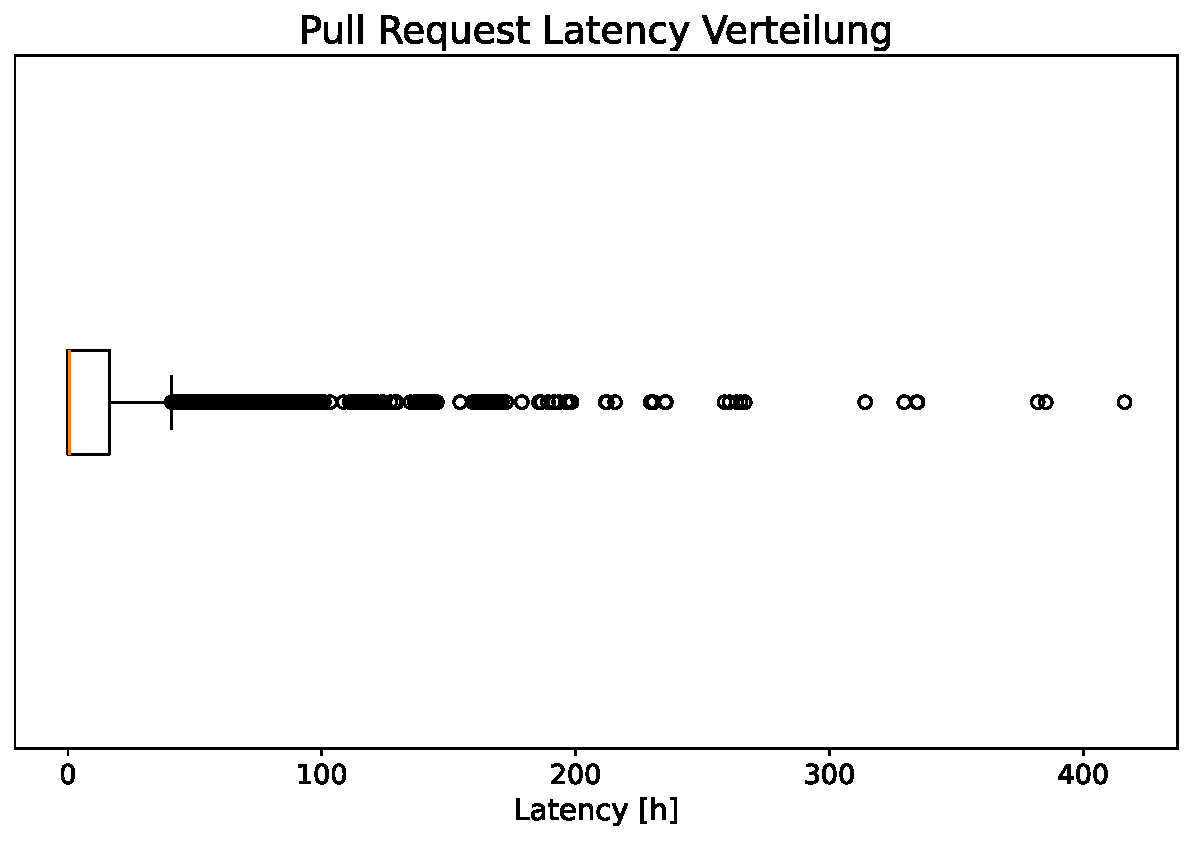
\includegraphics[width=0.8\textwidth]{Figures/boxplot-latency.pdf}
    \centering
    \caption{Verteilung der Latencies von den Pull-Requests}
    \label{fig:boxplot-latency}
\end{figure}

Der Boxplot in der \autoref{fig:boxplot-churn} zeigt, dass es viele kleine Pull-Requests mit wenigen Codezeilenänderungen gibt. Wie bereits bei der Latency wird festgestellt, dass es eine Reihe von Ausreissern gibt, von denen einige besonders hervorstechen. Diese befinden sich bei über 10'000 Zeilenänderungen. In diesem Fall liegt die Anzahl der Ausreisser bei 9.6\,\%.

\begin{figure}[htbp]
    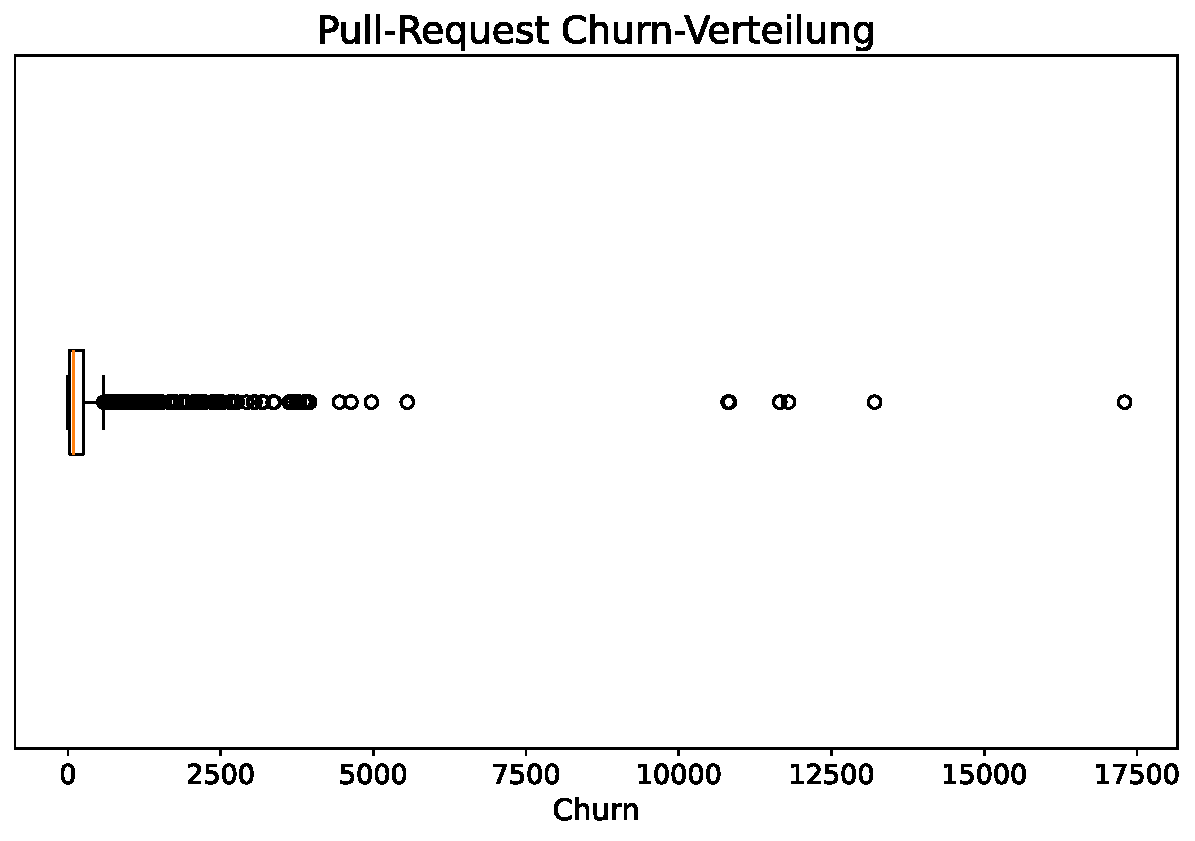
\includegraphics[width=0.8\textwidth]{Figures/boxplot-churn.pdf}
      \centering
    \caption{Verteilung der Churns von den Pull-Requests}
    \label{fig:boxplot-churn}
\end{figure}

Werden die Ausreisser beider Metriken kumulativ aus allen Datensätzen herausgefiltert, bleiben 1'887 Pull-Requests übrig, was 77.5\,\% entspricht. Das Herausfiltern dieser Daten stellt einen erheblichen Eingriff in die Datenbasis dar und wird daher nicht pauschal vorgenommen.

\subsection{Ergebnisse}
Um festzustellen, ob zwischen den Metriken Latency und Churn ein Zusammenhang besteht, wird die Spearman-Rangkorrelation angewendet. Dafür wird die oben erwähnte \autoref{eqn:spearman} verwendet. Diese wird mittels der Python-Bibliothek pandas berechnet. Als Ergebnis erreichte der Rangkorrelationskoeffizient einen Wert von 0.17. Dieser Wert liegt nahe bei null und zeigt somit keinen spezifischen Zusammenhang zwischen den beiden Metriken auf. 

Wie bereits erwähnt, weisen die Daten einen hohen Anteil an Ausreissern auf. Deshalb soll überprüft werden, ob die Metriken eine Korrelation besitzen, wenn diese Ausreisser herausgefiltert werden. In diesem Fall erhöht sich der Koeffizient auf 0.2, zeigt aber weiterhin keinen eindeutigen Zusammenhang zwischen den Metriken.

\subsection{Zusammenfassung}
Die Analyse zeigt, dass die meisten Pull-Requests sehr schnell bearbeitet werden, mit einer Median-Bearbeitungszeit von 0.6 Stunden. Der Churn verteilt sich ebenfalls sehr ungleich, die meisten PRs enthalten wenige Änderungen, einige jedoch sehr viele. Der Mittelwert der Anzahl Codeänderungen (Churn) liegt bei 278 Zeilen.

Die Berechnung der Spearman-Rangkorrelation ergibt einen Wert von 0.17, was auf keinen signifikanten Zusammenhang zwischen dem Churn und der Latency hindeutet. Auch nach Herausfiltern der Ausreisser bleibt der Zusammenhang mit 0.20 sehr schwach.
Zusammenfassend lässt sich zur \fref{forschungsfrage1} feststellen, dass die Metriken Latency und Churn, bei den untersuchten Projekten, keinen Zusammenhang aufweisen.

%----------------------------------------------------------------------------------------
% SECTION 2
%----------------------------------------------------------------------------------------
\section{Schliessungsgründe der Pull-Requests}
\label{sec:UntersuchungSchliessgründePRs} 
In diesem Abschnitt wird die \fref{forschungsfrage2} "\textit{Können die Schliessungsgründe der PRs in den Projekten ermittelt und klassifiziert werden?}" untersucht. Ziel ist es, die Gründe für die Ablehnung oder das Schliessen von PRs systematisch zu erfassen und im Hinblick auf \fref{forschungsfrage5} mögliche Muster zwischen Vollzeit- und Teilzeitklassen herauszuarbeiten.

\subsection{Kategorisierung der geschlossenen Pull-Requests}
\label{sec:KategorienGeschlossenePRs} 
Um die Ursache des geschlossenen PRs klassifizieren zu können, müssen zuerst Kategorien erstellt werden. Diese Kategorien wurden aufgrund einer manuellen Analyse des Datensatzes erreicht. 
Dafür wurden alle Pull-Requests der Racetrack-Repositories (Teilzeit sowie Vollzeit) ausgelesen und anschliessend eine Liste aller geschlossenen PRs mit einem Churn von mindestens 500 erstellt. Diese Liste umfasste 39 Pull-Requests. Um den Datensatz ausgewogener zu gestalten, wurde ergänzend eine zufällige Stichprobe von 20 weiteren geschlossenen PRs mit einem Churn von weniger als 500 ausgewählt und hinzugefügt. Im Folgenden sind die definierten Kategorien aufgeführt:

\begin{itemize}
    \item \textbf{PRs ohne erkennbaren Grund (OG)}: Die PRs wurden ohne Kommentar geschlossen.
    \item \textbf{Feature durch anderen PR implementiert (FPI)}: Das Feature wurde durch einen anderen PR implementiert und der ursprüngliche PR anschliessend geschlossen.
    \item \textbf{PRs mit falschem Zielbranch (FZB)}: Der Autor des PRs wählte den falschen Zielbranch aus. Der Branch wurde anschliessend mittels eines neuen PRs in den korrekten Zielbranch gemerged.
    \item \textbf{Feature wird nicht mehr benötigt (FNN)}: Das Feature wird nicht mehr benötigt. Dies muss explizit im PR vermerkt sein.
    \item \textbf{Implementierung abgelehnt (IA)}: Die vorgeschlagene Implementierung wurde abgelehnt.
    \item \textbf{Divers (DIV)}: Beinhaltet hauptsächlich Feedback-PRs, welche von gewissen Dozenten für die Notenvergabe verwendet wurden. Ausserdem sind einige Refactor-Branches zu sehen, welche ausschliesslich für das Refactoring erstellt wurden und anschliessend geschlossen wurden. 
\end{itemize}


\subsection{Deskriptive Analyse}
Insgesamt wurden 2'427 Pull-Requests untersucht, wovon 170 PRs geschlossen wurden (7.0 \%). Von den geschlossenen PRs entfielen 95 auf Vollzeitklassen und 75 auf Teilzeitklassen. Die Teilzeitklassen verfügen im Schnitt über 2.77 und die Vollzeitklassen 2.15 geschlossene PRs pro Projekt. 

Der durchschnittliche Churn bei geschlossenen PRs beträgt: \begin{itemize} \item Teilzeitklassen: 137 Zeilenänderungen \item Vollzeitklassen: 188 Zeilenänderungen \end{itemize}

Eine Aufteilung der geschlossenen Pull-Requests nach Churn-Grösse zeigt, dass in Teilzeitklassen vorwiegend kleinere PRs geschlossen wurden. In den Vollzeitklassen hingegen ist die Spannweite der Churn-Grössen etwas grösser, wie \autoref{fig:anz-clsd-prs-nach-churn} zeigt.

\begin{figure}[htbp]
    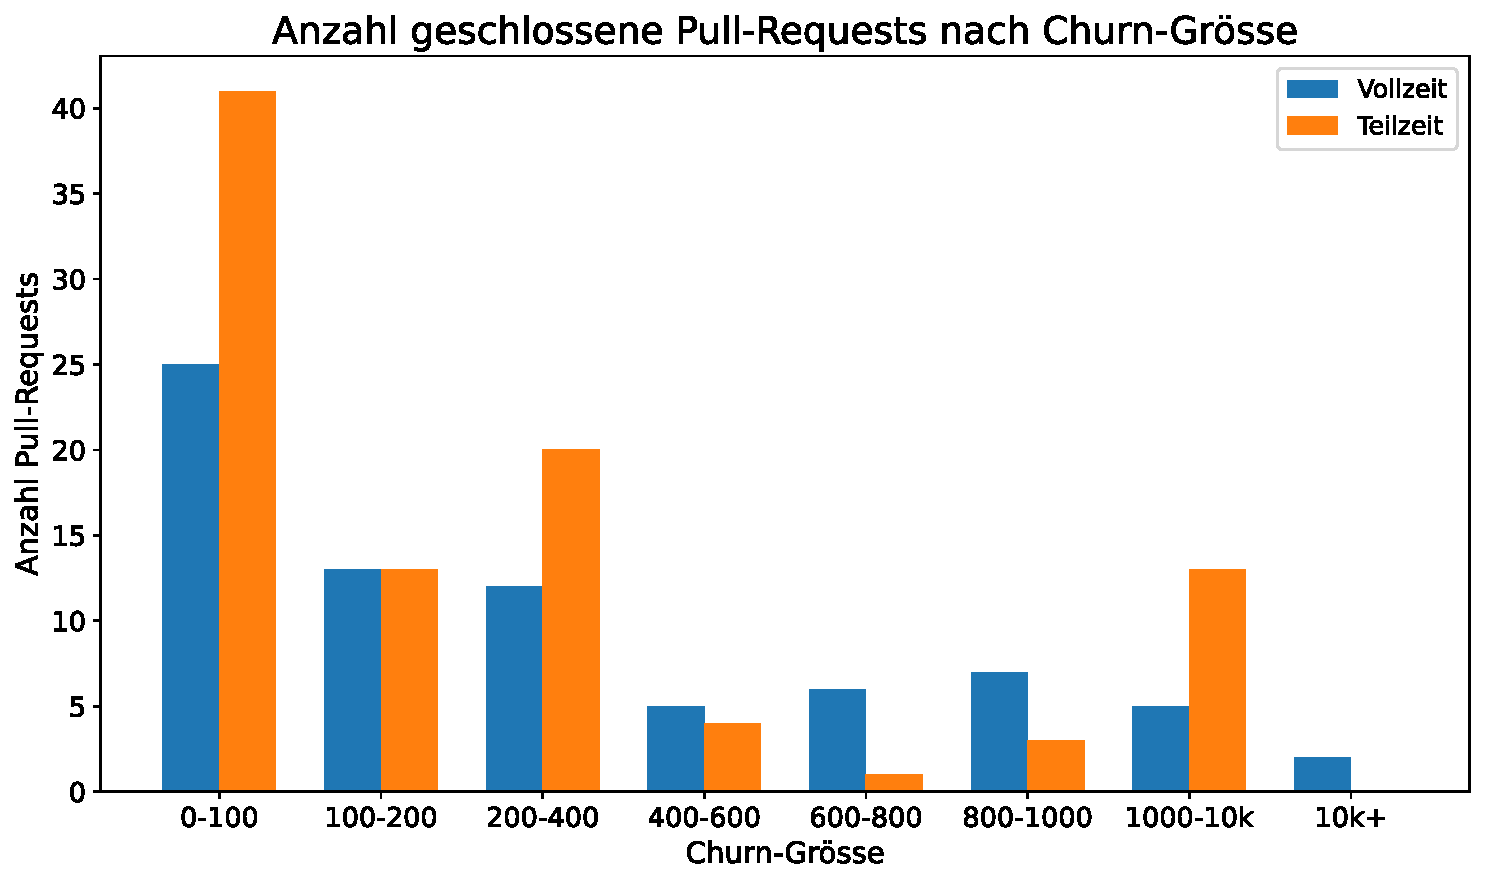
\includegraphics[width=\textwidth]{Figures/anzahl-geschlossene-prs-nach-churn.pdf}
    \caption{Anzahl geschlossene Pull-Requests nach Churn-Grösse}
    \label{fig:anz-clsd-prs-nach-churn}
\end{figure}


In \autoref{fig:avg-anz-clsd-prs-nach-churn} ist die durchschnittliche Anzahl geschlossener PRs pro Projekt für die Teilzeit- und Vollzeitklassen ersichtlich.

In der kleinsten Churn-Kategorie (0--100) ist die durchschnittliche Anzahl geschlossener PRs pro Repository mit 0.93 in beiden Gruppen nahezu gleich. Bei einem Churn von 100--200 liegt der Durchschnittswert in Vollzeitklassen mit 0.48 deutlich höher als in Teilzeitklassen mit 0.30. Im Bereich 200--400 gleichen sich die Werte mit rund 0.45 wieder an.

Für grössere Churn-Werte (400--800) sinkt die durchschnittliche Anzahl geschlossener PRs in beiden Gruppen deutlich, wobei Vollzeitklassen durchgehend höhere Werte aufweisen (z.\,B. bei 600--800: Teilzeit 0.02, Vollzeit 0.22). In den Kategorien oberhalb von Churn 800 sind fast keine PRs der Teilzeitklassen zu finden. Besonders bei einem Churn von über 10'000 treten nur noch bei Vollzeitklassen geschlossene PRs auf (Durchschnitt: 0.07), während dieser Wert bei Teilzeitklassen bei null liegt.

\begin{figure}[htbp]
    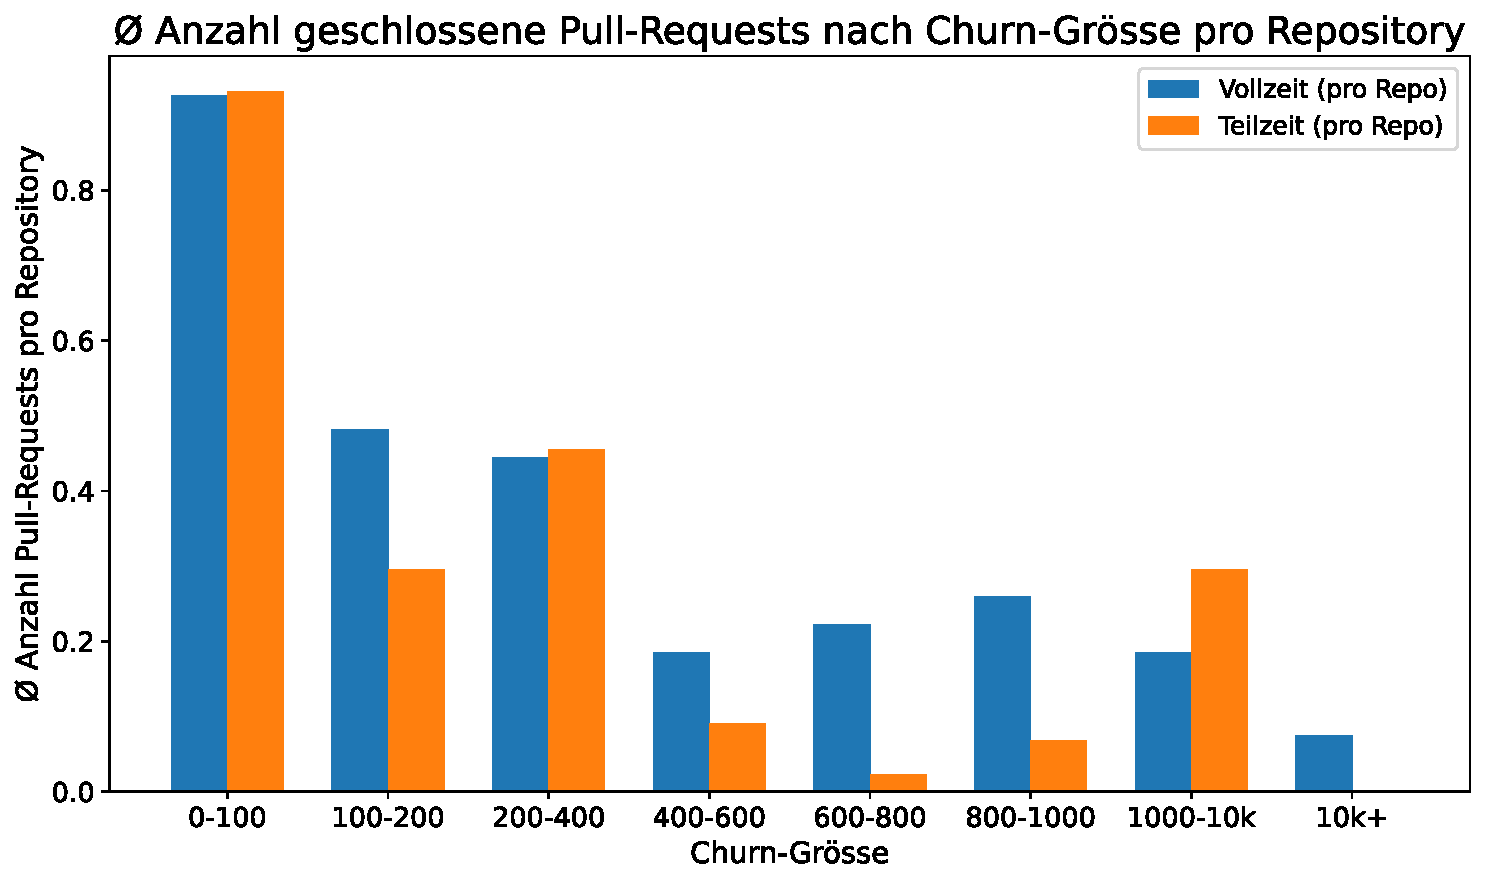
\includegraphics[width=\textwidth]{Figures/avg-anz-clsd-prs-nach-churn.pdf}
    \caption{Durchschnittliche Anzahl geschlossene Pull-Requests nach Churn-Grösse pro Repository}
    \label{fig:avg-anz-clsd-prs-nach-churn}
\end{figure}

Ergänzend zur durchschnittlichen Anzahl geschlossener PRs pro Projekt zeigt die \autoref{fig:vergleich-gesamtanzahl-prs-vs-closed-teilzeit}, wie sich die Gesamtzahl aller PRs und die Anzahl geschlossener PRs in den Teilzeitklassen über die verschiedenen Churn-Kategorien verteilt. Für die Vollzeitklassen findet sich in \autoref{fig:vergleich-gesamtanzahl-prs-vs-closed-vollzeit} die gleiche Darstellung.

\begin{figure}[htbp]
    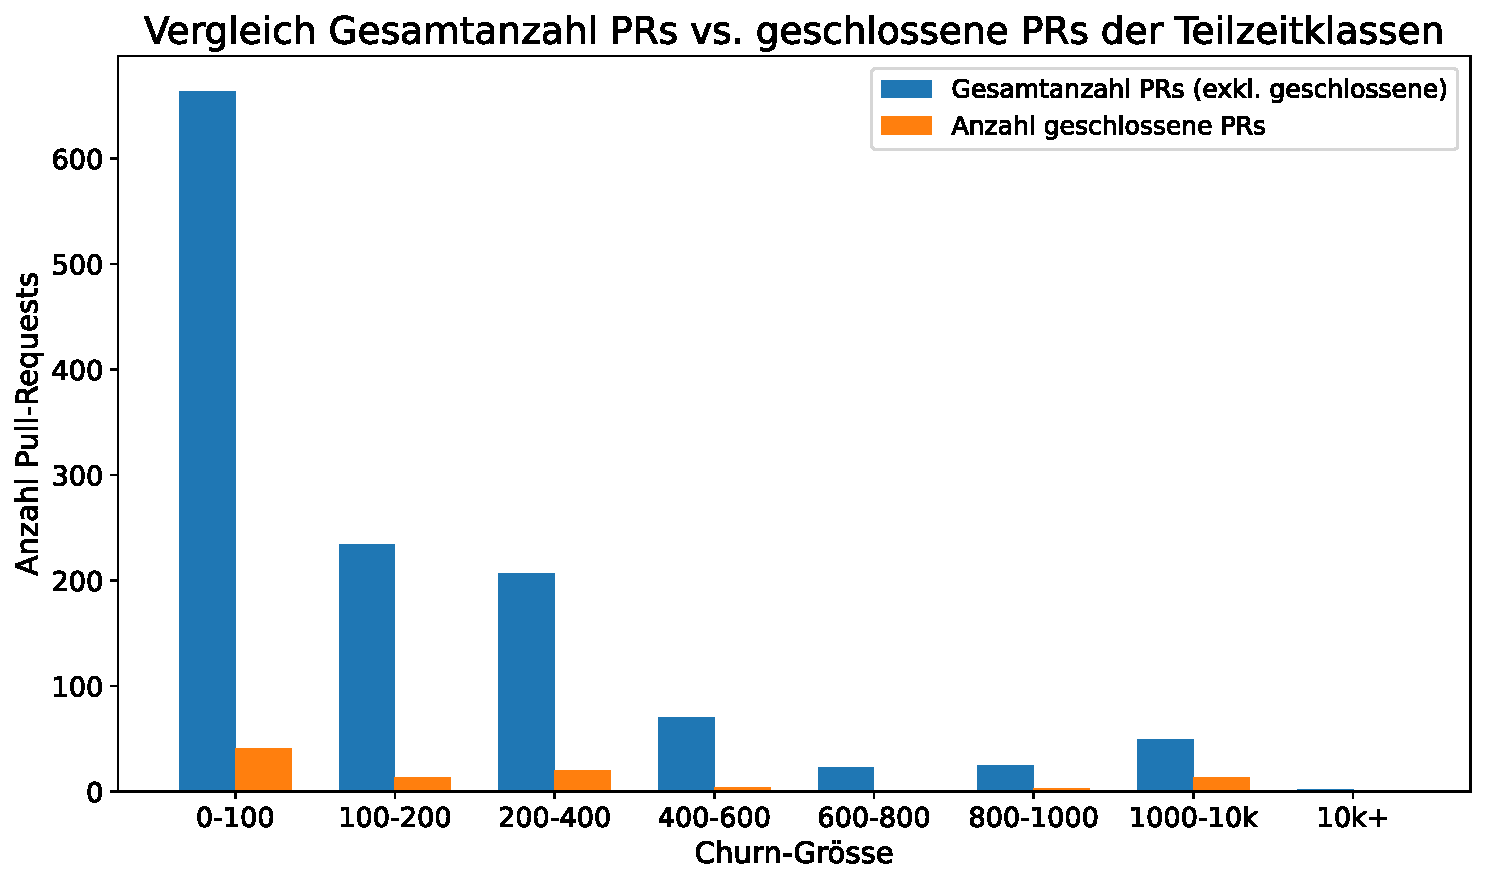
\includegraphics[width=\textwidth]{Figures/vergleich-gesamtanzahl-prs-vs-closed-teilzeit.pdf}
    \caption{Vergleich Gesamtanzahl PRs (exkl. geschlossene) vs. geschlossene PRs der Teilzeitklassen}
    \label{fig:vergleich-gesamtanzahl-prs-vs-closed-teilzeit}
\end{figure}


In beiden Unterrichtsformen zeigt sich, dass die Mehrheit der Pull-Requests in die kleinste Churn-Kategorie (0–100) fällt. Mit zunehmendem Churn nimmt sowohl die Gesamtanzahl der PRs als auch die Zahl der geschlossenen PRs kontinuierlich ab. Auffällig ist jedoch, dass bei den Vollzeitklassen auch in den höheren Churn-Kategorien mehr geschlossene Pull-Requests registriert sind. So finden sich etwa in der Kategorie 1'000–10k deutlich mehr geschlossene PRs als in den Teilzeitklassen, obwohl die Gesamtanzahl der PRs in diesem Bereich nur geringfügig höher ist.
In der höchsten Churn-Kategorie (>10k) sind in den Teilzeitklassen keine geschlossenen PRs zu verzeichnen, während in den Vollzeitklassen noch vereinzelte Schliessungen vorkommen. 

\begin{figure}[htbp]
    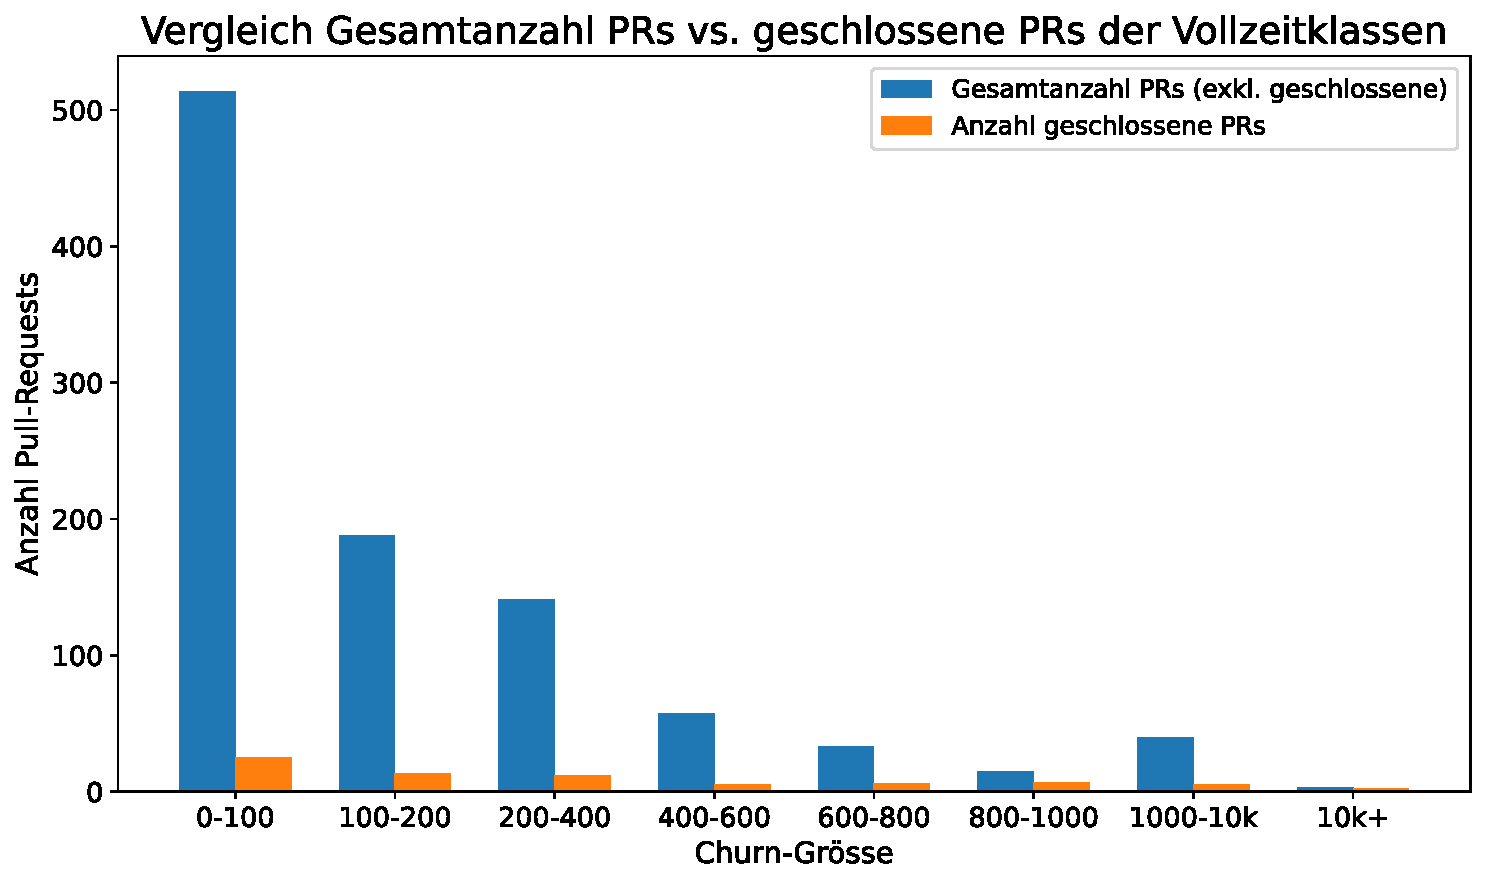
\includegraphics[width=\textwidth]{Figures/vergleich-gesamtanzahl-prs-vs-closed-vollzeit.pdf}
    \caption{Vergleich Gesamtanzahl PRs (exkl. geschlossene) vs. geschlossene PRs der Vollzeitklassen}
    \label{fig:vergleich-gesamtanzahl-prs-vs-closed-vollzeit}
\end{figure}


\subsection{Ursachenanalyse der geschlossenen PRs}
Für die Ursachenanalyse wurden alle PRs mit einem Churn-Wert grösser als 500 sowie alle mit einem Churn-Wert kleiner als 100 manuell untersucht und den in Kapitel \secref{sec:KategorienGeschlossenePRs} definierten Kategorien zugeordnet. 
Die Verteilung der Ursachen geschlossener PRs ist in \autoref{tab:geschlossene-prs-nach-ursache} dargestellt.


\begin{table}[htbp]
\caption{Geschlossene PRs gruppiert nach Ursache}
\label{tab:geschlossene-prs-nach-ursache}
\centering
\begin{tabular}{l l l l l l l}
\toprule
\textbf{Klasse} & 
\makecell{\textbf{OG}} & 
\makecell{\textbf{FPI}} & 
\makecell{\textbf{FNN}} & 
\makecell{\textbf{IA}} & 
\makecell{\textbf{FZB}} & 
\makecell{\textbf{DIV}} \\
\midrule
T < 100& 35 & 1 & 3 & 2 & 0 & 0\\
V < 100& 22 & 1 & 0 & 1 & 1 & 0 \\
T > 500& 22 & 8 & 0 & 2 & 4 & 5 \\
V > 500& 8 & 0 & 1 & 4 & 6 & 0 \\
\bottomrule
\end{tabular}
\end{table}

\newpage
\textbf{Legende:}

\noindent
\begin{minipage}[t]{0.3\textwidth}
\begin{tabular}{r l}
$T$ & Alle Teilzeitklassen \\
$V$ & Alle Vollzeitklassen \\
$< 100$ & Churn kleiner 100 \\
$> 500$ & Churn grösser 500 \\
\end{tabular}
\end{minipage}
\hfill
\begin{minipage}[t]{0.6\textwidth}
\begin{tabular}{r l}
$OG$ & PRs ohne erkennbaren Grund \\
$FPI$ & Feature durch anderen PR im\-plementiert \\
$FZB$ & PRs mit falschem Zielbranch \\
$FNN$ & Feature wird nicht mehr benötigt \\
$IA$ & Implementierung abgelehnt  \\
$DIV$ & Divers \\
\end{tabular}
\end{minipage}


Zur besseren visuellen Veranschaulichung dient \autoref{fig:anz-clsd-prs-nach-ursache-und-churn}, welche die \autoref{tab:geschlossene-prs-nach-ursache} darstellt.


\begin{figure}[htbp]
    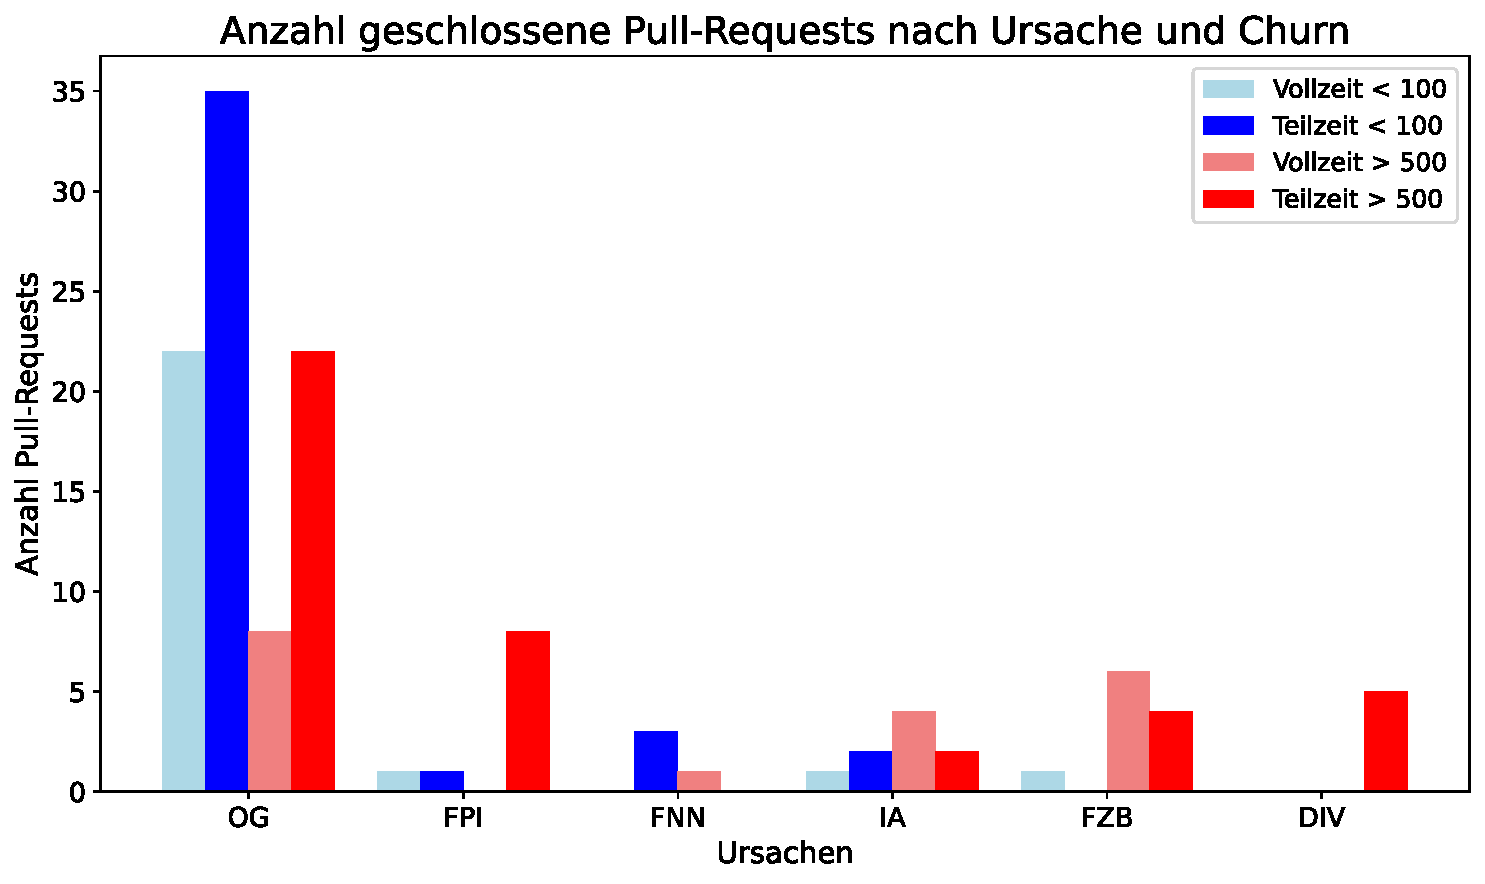
\includegraphics[width=\textwidth]{Figures/ursachenanalyse.pdf}
    \caption{Geschlossene PRs gruppiert nach Ursache}
    \label{fig:anz-clsd-prs-nach-ursache-und-churn}
\end{figure}
So ist in der \autoref{tab:geschlossene-prs-nach-ursache} und \autoref{fig:anz-clsd-prs-nach-ursache-und-churn} sichtbar, dass die meisten PRs in allen Klassen jeweils ohne erkennbaren Grund OG geschlossen werden. Dieses Muster ist insbesondere bei den PRs mit einem geringen Churn (<100) ausgeprägt, wobei bei beiden Unterrichtsmodellen ein klarer Spitzenwert in dieser Kategorie erkennbar ist.


Bei PRs mit einem grossen Churn (>500) hingegen zeigt sich eine leicht stärkere Differenzierung der Schliessgründe.
In den Vollzeitklassen treten dabei strukturierte Ursachen wie FZB (falscher Zielbranch) und IA (Implementierung abgelehnt) auf. 
In den Teilzeitklassen hingegen treten im Bereich grosser PRs vermehrt Ursachen der Kategorie FPI (Feature durch anderen PR implementiert) oder in der Kategorie DIV auf, welche unter anderem Refactorings und Feedback-PRs beinhalten.


Die Normalisierung der Daten erfolgt, indem die absolute Anzahl geschlossener Pull-Requests jeder Ursache durch die Anzahl der analysierten Repositories innerhalb der jeweiligen Unterrichtsform dividiert wird. Dadurch entsteht ein durchschnittlicher Wert pro Repository, der eine vergleichbare Betrachtung zwischen Voll\-zeit- und Teilzeitklassen ermöglicht. \autoref{tab:durchschittliche-anzahl-geschlossene-prs-nach-ursache-pro-projekt} zeigt die durchschnittlichen geschlossenen PRs gruppiert nach Ursache und Churn pro Projekt.  

In den beiden Churn-Klassen (<100) ist die Ursache OG (ohne erkennbaren Grund) mit Abstand am häufigsten vertreten. In Vollzeit- und Teilzeitklassen liegt der durchschnittliche Wert jeweils bei rund 0.8 geschlossenen PRs pro Repository. Auch bei PRs mit grossem Churn (> 500) bleibt OG die häufigste Ursache.

Strukturierte Ursachen wie FPI (Feature durch anderen PR implementiert), IA (Implementierung abgelehnt) und FZB (falscher Zielbranch) treten bei PRs mit grossem Churn in beiden Unterrichtsformen auf, in Vollzeitklassen jedoch oftmals mit höheren Durchschnittswerten. Für FZB beträgt der Durchschnitt in Vollzeitklassen 0.222 PRs pro Repository, in Teilzeitklassen 0.091. Die Ursache FPI tritt ausschliesslich in Teilzeitklassen auf (0.182), IA hingegen ist in Vollzeitklassen mit 0.148 stärker vertreten als in Teilzeitklassen (0.045). Die Kategorie DIV, welche unter anderem Refactor- und Feedback-PRs umfasst, ist nur in Teilzeitklassen mit grossem Churn vertreten und besitzt dort einen durchschnittlichen Wert von 0.114 PRs pro Repository.

Die Ursache FNN (Feature wird nicht mehr benötigt) zeigt ein etwas anderes Bild: Sie ist bei kleinen PRs (Churn < 100) ausschliesslich in Teilzeitklassen mit einem Durchschnitt von 0.068 vertreten und ist bei den Vollzeitklassen nicht vertreten. Bei einem Churn (> 500) ist FNN nur in den Vollzeitklassen mit einem Wert von 0.037 vertreten und in den Teilzeitklassen nicht vorhanden.

\begin{table}[htbp]
\caption{Durchschnittliche Anzahl geschlossene PRs gruppiert nach Ursache und Churn pro Repository}
\label{tab:durchschittliche-anzahl-geschlossene-prs-nach-ursache-pro-projekt}
\centering
\begin{tabular}{l l l l l l l}
\toprule
\textbf{Klasse} & 
\makecell{\textbf{OG}} & 
\makecell{\textbf{FPI}} & 
\makecell{\textbf{FNN}} & 
\makecell{\textbf{IA}} & 
\makecell{\textbf{FZB}} & 
\makecell{\textbf{DIV}} \\
\midrule
T < 100 & 0.795 & 0.023 & 0.068 & 0.045 & 0.000 & 0.000 \\
V < 100 & 0.815 & 0.037 & 0.000 & 0.037 & 0.037 & 0.000 \\
T > 500 & 0.500 & 0.182 & 0.000 & 0.045 & 0.091 & 0.114 \\
V > 500 & 0.296 & 0.000 & 0.037 & 0.148 & 0.222 & 0.000 \\
\bottomrule
\end{tabular}
\end{table}
\textbf{Legende:}

\noindent
\begin{minipage}[t]{0.3\textwidth}
\begin{tabular}{r l}
$T$ & Alle Teilzeitklassen \\
$V$ & Alle Vollzeitklassen \\
$< 100$ & Churn kleiner 100 \\
$> 500$ & Churn grösser 500 \\
\end{tabular}
\end{minipage}
\hfill
\begin{minipage}[t]{0.6\textwidth}
\begin{tabular}{r l}
$OG$ & PRs ohne erkennbaren Grund \\
$FPI$ & Feature durch anderen PR im\-plementiert \\
$FZB$ & PRs mit falschem Zielbranch \\
$FNN$ & Feature wird nicht mehr benötigt \\
$IA$ & Implementierung abgelehnt  \\
$DIV$ & Divers \\
\end{tabular}
\end{minipage}
\\

Als visuelle Darstellung der \autoref{tab:durchschittliche-anzahl-geschlossene-prs-nach-ursache-pro-projekt} dient die \autoref{fig:avg-avg-anz-clsd-prs-nach-ursache-und-churn}.

\begin{figure}[htbp]
    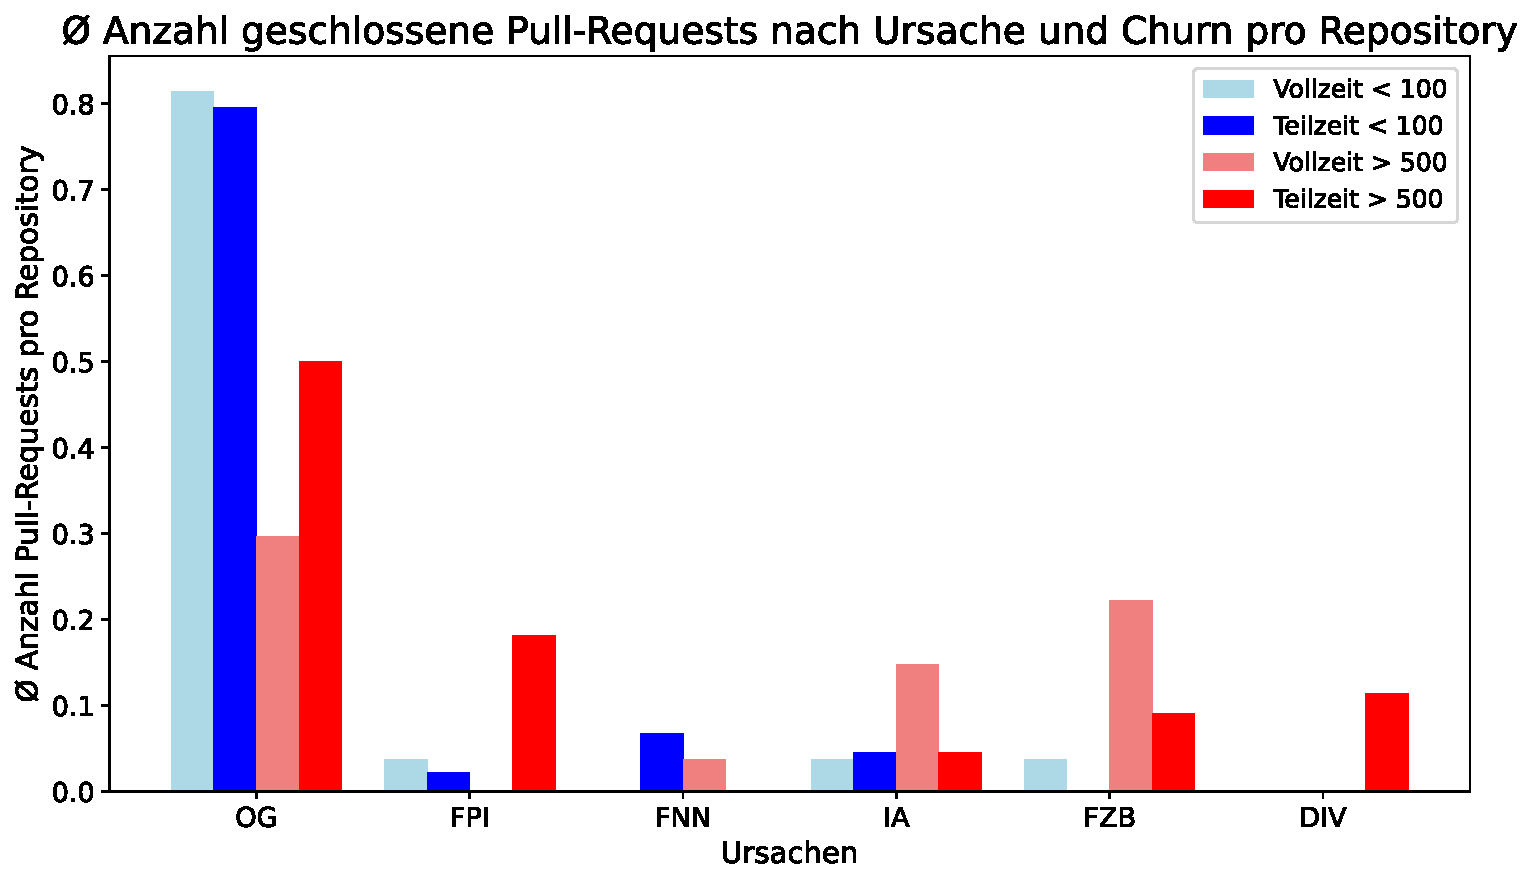
\includegraphics[width=\textwidth]{Figures/ursachenanalyse-pro-repo.pdf}
    \caption{Durchschnittliche Anzahl geschlossene PRs gruppiert nach Ursache und Churn pro Repository}
    \label{fig:avg-avg-anz-clsd-prs-nach-ursache-und-churn}
\end{figure}

Zusammenfassend zeigen die Ergebnisse, dass bei kleinen Pull-Requests (Churn < 100) die Ursache OG (ohne erkennbaren Grund) in beiden Unterrichtsformen mit Abstand am häufigsten vorkommt. Bei grossen Pull-Requests (Churn > 500) verteilt sich die Anzahl geschlossener PRs auf mehrere Ursachen. In Vollzeitklassen treten in dieser Churn-Kategorie strukturierte Ursachen wie IA (Implementierung abgelehnt), FZB (falscher Zielbranch) und FNN (Feature wird nicht mehr benötigt) häufiger auf. In Teilzeitklassen hingegen ist die Ursache FPI (Feature durch anderen PR implementiert) nur in dieser Unterrichtsform vertreten. Zudem tritt die Kategorie DIV, welche unter anderem Feedback- und Refactoring-PRs umfasst, ausschliesslich in Teilzeitklassen mit grossem Churn auf. Die dargestellten Trends zeigen sich sowohl in den absoluten Werten als auch in den normalisierten Daten pro Repository.

\subsection{Zeitliche Analyse geschlossener PRs}

Eine Analyse der geschlossenen PRs im zeitlichen Verlauf der Projektlaufzeit zeigt deutliche Unterschiede zwischen Vollzeit- und Teilzeitklassen, wie in \autoref{fig:closed-prs-projektzeit} ersichtlich.

\begin{figure}[htbp] 
\centering \begin{subfigure}[b]{0.48\textwidth} 
\centering 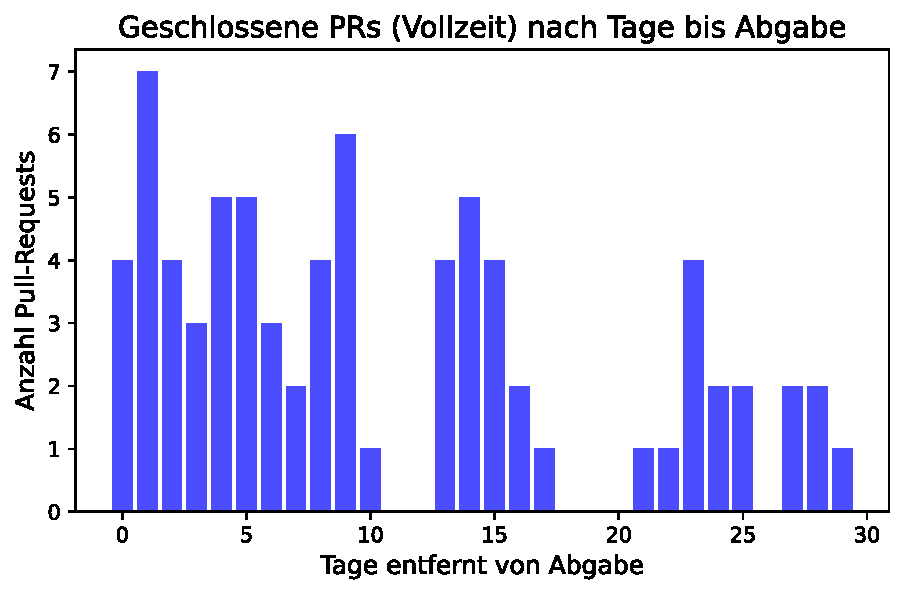
\includegraphics[width=\textwidth]{Figures/closed-prs-projektzeit-vollzeit.pdf} 
\caption{Geschlossene PRs Vollzeitklassen} 
\label{fig:closed-prs-projektkeit-vollzeit}
\end{subfigure} 
\hfill 
\begin{subfigure}[b]{0.48\textwidth} 
\centering 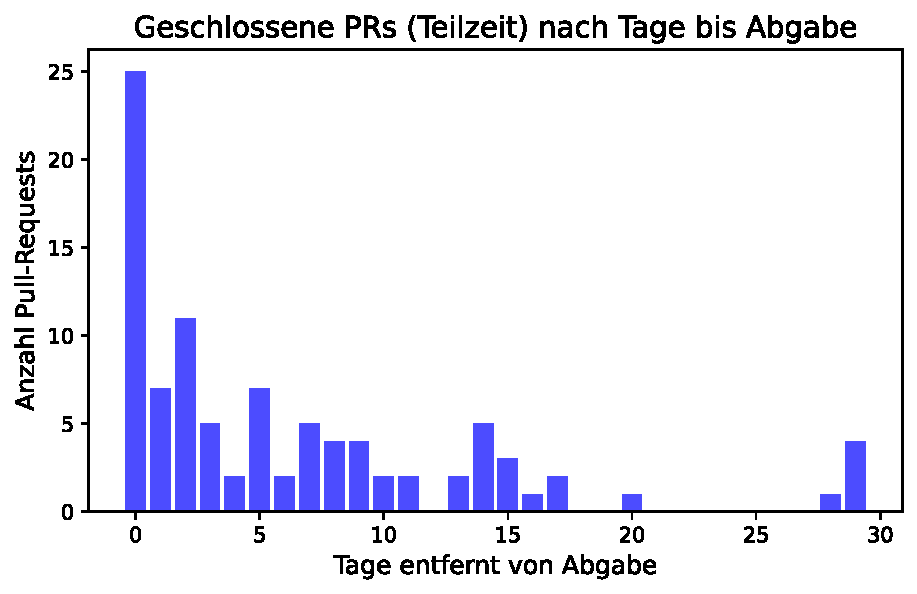
\includegraphics[width=\textwidth]{Figures/closed-prs-projektzeit-teilzeit.pdf} 
\caption{Geschlossene PRs Teilzeitklassen} 
\label{fig:closed-prs-projektkeit-teilzeit} 
\end{subfigure} 
\caption{Anzahl geschlossener PRs nach Tagen vor Abgabetermin} 
\label{fig:closed-prs-projektzeit} 
\end{figure}


Die wichtigsten Beobachtungen sind folgende: In Teilzeitklassen konzentrieren sich die geschlossenen PRs stark auf die letzten Projekttage, insbesondere auf den Tag der Abgabe. In Vollzeitklassen hingegen verteilen sich die geschlossenen PRs gleichmässiger über den gesamten Projektverlauf.


\subsection{Zusammenfassung}

Zusammenfassend lässt sich festhalten, dass sich die Schliessgründe von Pull-\linebreak Requests nicht eindeutig klassifizieren lassen. Viele PRs wurden ohne erkennbaren Grund geschlossen, insbesondere bei kleineren Änderungen mit einem Churn unter 100. Dieses Verhalten tritt besonders häufig bei den Teilzeitklassen auf. Auffällig ist dabei, dass diese oft ohne Begründung geschlossen werden. Zudem werden viele PRs der Teilzeitklassen erst gegen Ende des Projekts, besonders am Abgabetag, geschlossen.

Im Gegensatz dazu zeigen Vollzeitklassen bei den grossen Pull-Requests häufiger strukturierte Schliessgründe wie falsche Zielbranches oder abgelehnte Implementierungen. Sie korrigieren grössere PRs zudem häufiger gezielt, anstatt sie kommentarlos zu schliessen. Insgesamt werden in den Vollzeitklassen durchschnittlich mehr PRs pro Projekt geschlossen. Zudem sind Schliessungen hier gleichmässiger über den gesamten Projektverlauf verteilt. Darüber hinaus zeigt sich, dass bei PRs mit hohen Churn-Werten Schliessungen häufiger auf Branch-Fehler oder redundante Implementierungen zurückzuführen sind.

%----------------------------------------------------------------------------------------
% SECTION 3
%----------------------------------------------------------------------------------------
\section{Einfluss von Projektzeit}
Als Nächstes wurde die \fref{forschungsfrage3} "\textit{Besteht ein Zusammenhang zwischen dem Zeitpunkt im Projektverlauf und der Review-Dauer von Pull-Requests?}" untersucht. Um zu ermitteln, ob die fortschreitende Projektzeit einen Einfluss auf das Bearbeiten der Pull-Requests hat. Zusätzlich werden auch die Churns untersucht, um zu sehen, wie sich diese im Verlauf der Projektzeit verändern. 


Ein signifikanter Faktor, der bei den Projektmodulen eine Rolle spielt, ist der fest definierte Abgabetermin. Dies unterscheidet diese Projekte von Open-Source-Projek\-ten, die in der Literatur häufig untersucht werden. Um diese Untersuchung durchführen zu können, wird zusätzlich zu den oben genannten Metriken der Abgabetermin der einzelnen Klassen nachgeschlagen.

Zur initialen Analyse wurden die Projekte in die entsprechenden Projektwochen aufgeteilt und die Mediane der Latencies und Churns der entsprechenden Wochen ermittelt. Dies soll eine allgemeine Übersicht der Veränderungen der Metriken aufzeigen.

\subsection{Projektwochen im Verhältnis zu Latency und Churn}
\label{sec:ProjektwochenLatencyChurn}
Die Woche, in der ein Pull-Request stattfindet, wird anhand der Metriken Pull-Request createTime und Repository createTime aus Kapitel~\secref{sec:Metriken} ermittelt. Dabei wird die Erstellungszeit des Repositories von der Eröffnungszeit des Pull-Requests abgezogen.

Anhand der \autoref{fig:mittelwert-woche-lateny} ist ersichtlich, dass die Latency gegen Ende der Projektzeit abnimmt, während den Churn (\autoref{fig:mittelwert-woche-churn}) bis zur 5. Woche ansteigt. 
Zu beachten ist, dass, wie bereits im Kapitel \secref{sec:Projektmodule} erwähnt, die Projekte nicht exakt 28 Tage dauern. Die ermittelten Projektlaufzeiten liegen zwischen 20 und 36 Tagen.
Wobei die Klassen aus den Jahren 2021 und 2022 bei einem Durchschnitt von 21 Tagen liegen. Die neueren Klassen ab dem Jahr 2023 haben eine Projektlaufzeitspannweite von 28 bis 36 Tagen, wobei eine Klasse 35 Tage überschreitet. In dieser Klasse haben fünf Teams eine Laufzeit von 29 Tagen und drei Teams eine Laufzeit von 35 oder 36 Tagen. Somit widerspiegeln diese drei Teams die Woche sechs in der folgenden \autoref{fig:vergleich-latency-churn-projektzeit}. Die Latency nimmt im Laufe der Zeit zweimal stark ab. Das erste Mal von der ersten zur zweiten Projektwoche, wobei sie in der ersten Woche bei einem Median von 3.5 Stunden und in der zweiten Woche bei 2 Stunden liegt. Zum zweiten Mal nimmt die Latency in der vierten Projektwoche stark ab, und zwar von 1.7 Stunden auf 0.5 Stunden. In der sechsten Woche ist die Latency nahezu 0. Der Churn steigt bis zur 5. Woche kontinuierlich von 72 Zeilenwechseln auf 115 an und sinkt dann in der 6. Woche auf 98.
\begin{figure}[htbp]
    \centering
    \begin{subfigure}[b]{0.48\textwidth}
        \centering
        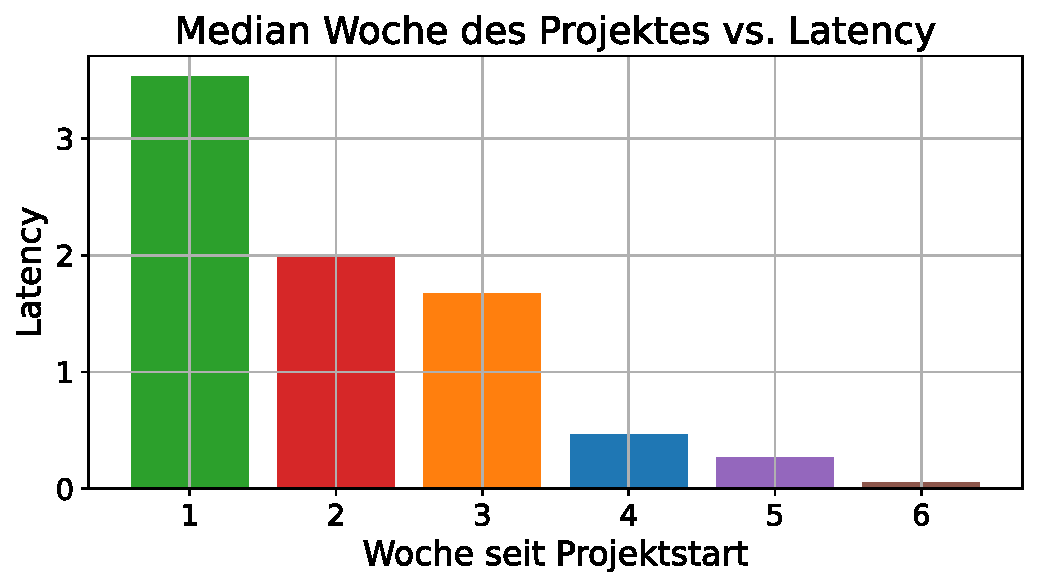
\includegraphics[width=\textwidth]{Figures/mittelwert-woche-latency.pdf}
        \caption{Mediane Woche des Projektes vs. Latency}
        \label{fig:mittelwert-woche-lateny}
    \end{subfigure}
    \hfill
    \begin{subfigure}[b]{0.48\textwidth}
        \centering
        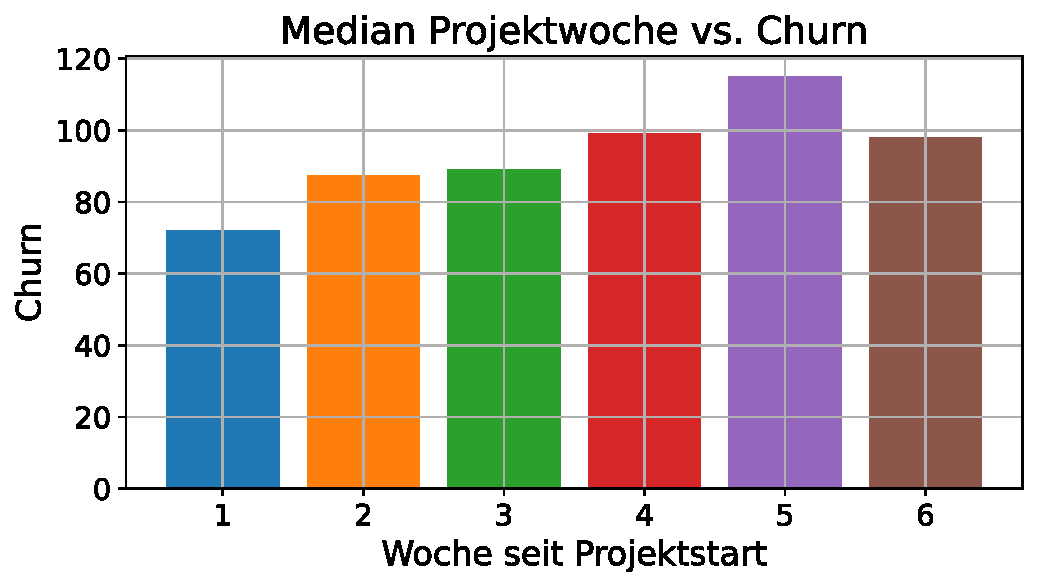
\includegraphics[width=\textwidth]{Figures/mittelwert-woche-churn.pdf}
        \caption{Mediane Woche des Projektes vs. Churn}
        \label{fig:mittelwert-woche-churn}
    \end{subfigure}
    \caption{Vergleich von Latency und Churn innerhalb der Projektzeit}
    \label{fig:vergleich-latency-churn-projektzeit}
\end{figure}

Werden die Daten nach Vollzeit- und Teilzeitstudierenden aufgeteilt, zeigt sich bei den Vollzeitklassen ein ähnliches Bild. Dies wird in der \autoref{fig:vergleich-latency-churn-projektzeit-v} veranschaulicht. Allerdings ist der Median der Latency in der ersten Woche mit 7.4 Stunden mehr als doppelt so hoch wie in der Gesamtauswertung. Ebenso nimmt die Latency von der ersten zur zweiten Woche stark ab. Der Wert sinkt um mehr als die Hälfte und liegt anschliessend bei 3.4 Stunden. Ab der vierten Woche ist der Median unter einer halben Stunde. Zeitgleich ist der Churn in der ersten Woche mit 71 Zeilenänderungen am geringsten, steigt mit Ausnahme der dritten Woche an und erreicht in der fünften Woche mit 121 Änderungen seinen Höhepunkt. Im Gegensatz zur Latency liegen diese Werte sehr nahe bei der Gesamtanalyse.
\begin{figure}[htbp]
    \centering
    \begin{subfigure}[b]{0.48\textwidth}
        \centering
        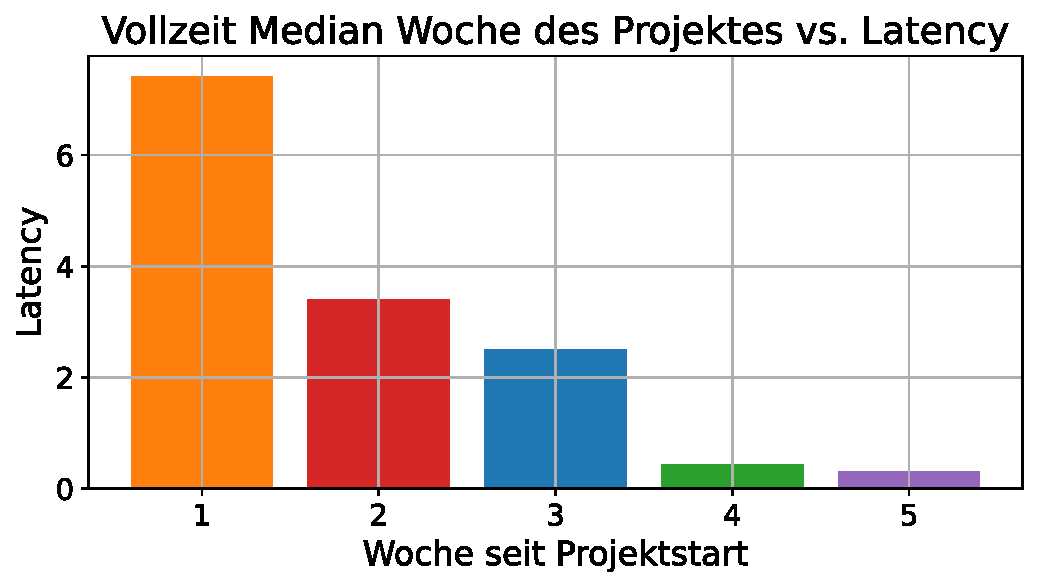
\includegraphics[width=\textwidth]{Figures/mittelwert-woche-latency-v.pdf}
        \caption{Mediane Woche des Projektes vs. Latency Vollzeit}
        \label{fig:mittelwert-woche-lateny-v}
    \end{subfigure}
    \hfill
    \begin{subfigure}[b]{0.48\textwidth}
        \centering
        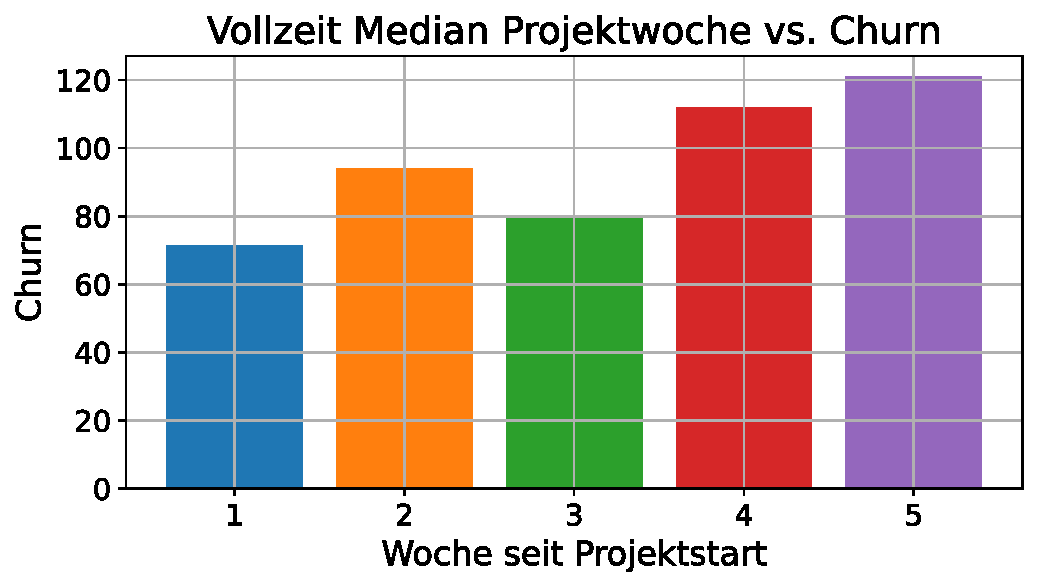
\includegraphics[width=\textwidth]{Figures/mittelwert-woche-churn-v.pdf}
        \caption{Mediane Woche des Projektes vs. Churn Vollzeit}
        \label{fig:mittelwert-woche-churn-v}
    \end{subfigure}
    \caption{Vergleich von Latency und Churn innerhalb der Projektzeit Vollzeit}
    \label{fig:vergleich-latency-churn-projektzeit-v}
\end{figure}

In der \autoref{fig:vergleich-latency-churn-projektzeit-t} ist zu erkennen, dass auch bei den Teilzeitstudierenden die Latency in der ersten Woche am höchsten ist, sich aber weniger stark von den Wochen zwei und drei unterscheidet. Zusätzlich ist der Wert der ersten Woche im Gegensatz zur Gesamtanalyse und vor allem den Vollzeitstudierenden tiefer bei einem Wert von knapp 2 Stunden. Zudem steigt bei den Teilzeitklassen in der dritten Woche die Latency nochmals an, aber dies nur mit einem Unterschied von 0.1 Stunden. Danach sinkt die Latency ebenso und liegt in Woche vier unter einer Stunde. Der Churn steigt ebenfalls an und erreicht in Woche fünf seinen Höhepunkt bei 110 Codezeilenänderungen. Die Werte der Churn befinden sich im gleichen Rahmen wie bei den Vollzeitstudierenden.

\begin{figure}[htbp]
    \centering
    \begin{subfigure}[b]{0.48\textwidth}
        \centering
        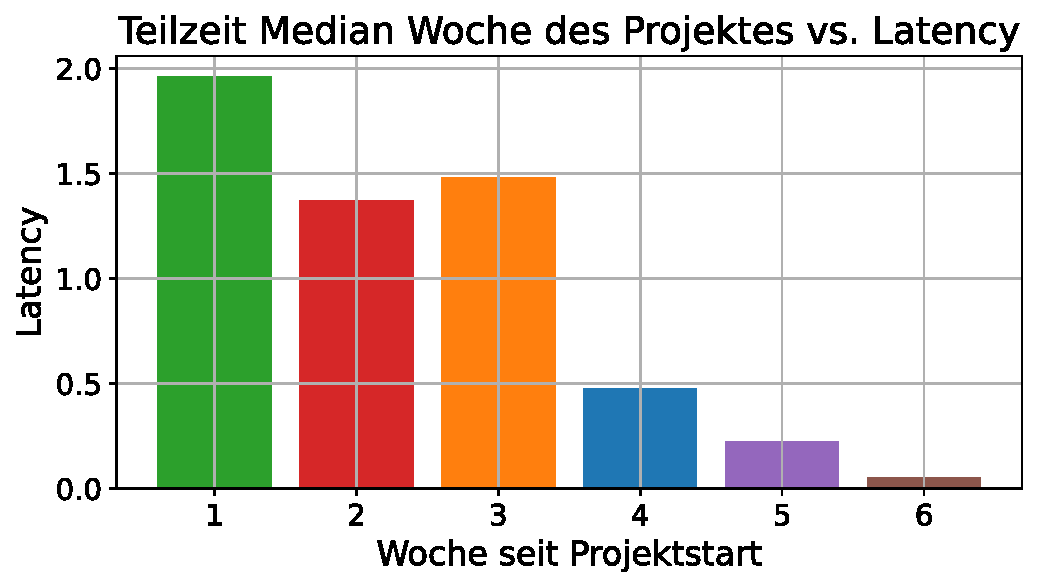
\includegraphics[width=\textwidth]{Figures/mittelwert-woche-latency-t.pdf}
        \caption{Mediane Woche des Projektes vs. Latency Teilzeit}
        \label{fig:mittelwert-woche-lateny-t}
    \end{subfigure}
    \hfill
    \begin{subfigure}[b]{0.48\textwidth}
        \centering
        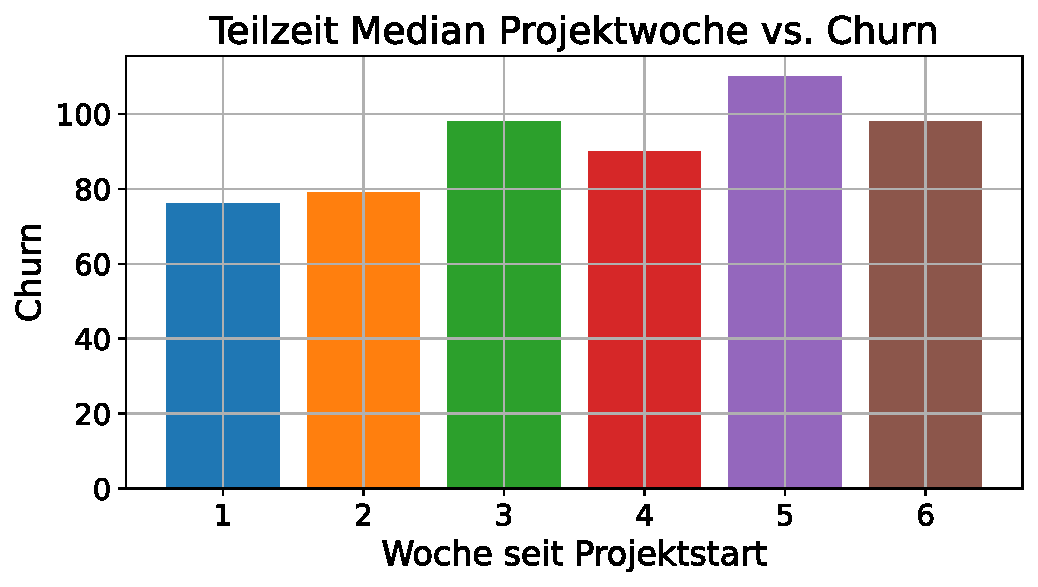
\includegraphics[width=\textwidth]{Figures/mittelwert-woche-churn-t.pdf}
        \caption{Mediane Woche des Projektes vs. Churn Teilzeit}
        \label{fig:mittelwert-woche-churn-t}
    \end{subfigure}
    \caption{Vergleich von Latency und Churn innerhalb der Projektzeit Teilzeit}
    \label{fig:vergleich-latency-churn-projektzeit-t}
\end{figure}

Zusammenfassend lässt sich feststellen, dass die Latency im Laufe der Zeit abnimmt, während der Churn zunimmt. Es ist auch ersichtlich, dass Vollzeitstudierende vor allem in der ersten Woche einen deutlich höheren Wert bei der Bearbeitungszeit der Pull-Requests haben. Zu beachten ist jedoch, dass, wie bereits erwähnt, nicht alle Projekte gleich lange dauerten. Somit waren in den Wochen vier, fünf und sechs nicht mehr alle Projekte aktiv. Deshalb wurde zusätzlich ermittelt, wie die Pull-Request-Verteilung über die Projektwochen ist.

Wie in der \autoref{tab:anz_pr_per_week} ersichtlich, wurden die wenigsten Pull-Requests in der sechsten Woche erstellt. Zu diesem Zeitpunkt liefen jedoch nur noch drei Projekte. Abgesehen davon werden in der ersten Projektwoche die wenigsten Pull-Requests erstellt. Diese Zahl steigt dann kontinuierlich bis zur 4. Woche an, obwohl in der 4. Woche nicht mehr alle Projekte am Laufen waren. In der fünften Woche ist ein Rückgang der Pull-Requests zu beobachten, wobei diese in der Gesamtzahl nur geringfügig unter der dritten Woche und bei den Teilzeitstudierenden sogar leicht darüber liegt. 

\begin{table}[ht]
\caption{Anzahl Pull-Requests pro Woche}
\label{tab:anz_pr_per_week}
\centering
\begin{tabular}{rrrr}
\toprule
\textbf{Woche} & \textbf{Vollzeit} & \textbf{Teilzeit} & \textbf{Gesamt} \\
\midrule
1 & 94 & 107 & 201 \\
2 & 158 & 174 & 332\\
3 & 275 & 317 & 592\\
4 & 298 & 363 & 661\\
5 & 241 & 341 & 582 \\
6 & 0 & 67 & 67\\
\bottomrule
\end{tabular}
\end{table}

Die Erstellung von Pull-Requests ist in den letzten Wochen der Projekte sehr hoch. Allerdings ist nicht genau ersichtlich, wie sich die Pull-Requests über die Laufzeit der einzelnen Projekte verteilen. Deshalb wird in einer weiteren Untersuchung analysiert, wie die Verteilung der Pull-Requests im Verhältnis zu den Abgabefristen der einzelnen Projekte aussieht. Es gilt zu beachten, dass bei Projekten zunächst meist die Konzeption erfolgt und die Studierenden das Klassendesign sowie das Testkonzept definieren. Dies könnte sich auf die Anzahl der Pull-Requests zu Beginn des Projekts auswirken.

\subsection{Pull-Requests im Verhältnis zum Abgabetermin}
Die Untersuchung von Pull-Requests im Verhältnis zur Abgabe zeigt, dass am Tag der Abgabe die meisten Pull-Requests abgearbeitet werden. Dies ist aus der \autoref{fig:anz-prs-days-away-from-end} ersichtlich. Von den 2427 untersuchten Pull-Requests wurden 523 am Tag der Abgabe erstellt und abgeschlossen. Dieser Wert entspricht einer Quote von 21.5\,\%.  Die zweitmeisten Pull-Requests wurden am Tag vor der Abgabe bearbeitet mit einer Anzahl von 309. Am drittletzten Tag wurde ein erhöhter Wert festgestellt, der jedoch nicht mehr signifikant hervorsticht. Eine Zusammenfassung der letzten drei Tage der Projekte ergibt eine Gesamtzahl von 986 bearbeiteten Pull-Requests, was einem Prozentsatz von 40.6\,\% entspricht. Über die restliche Projektzeit variieren die Anzahl bearbeiteter Pull-Requests. Es lassen sich erhöhte Werte sieben, acht und 15 Tage vor der Abgabe feststellen, die sich von den Werten der übrigen Tage abheben.
\begin{figure}[htbp]
    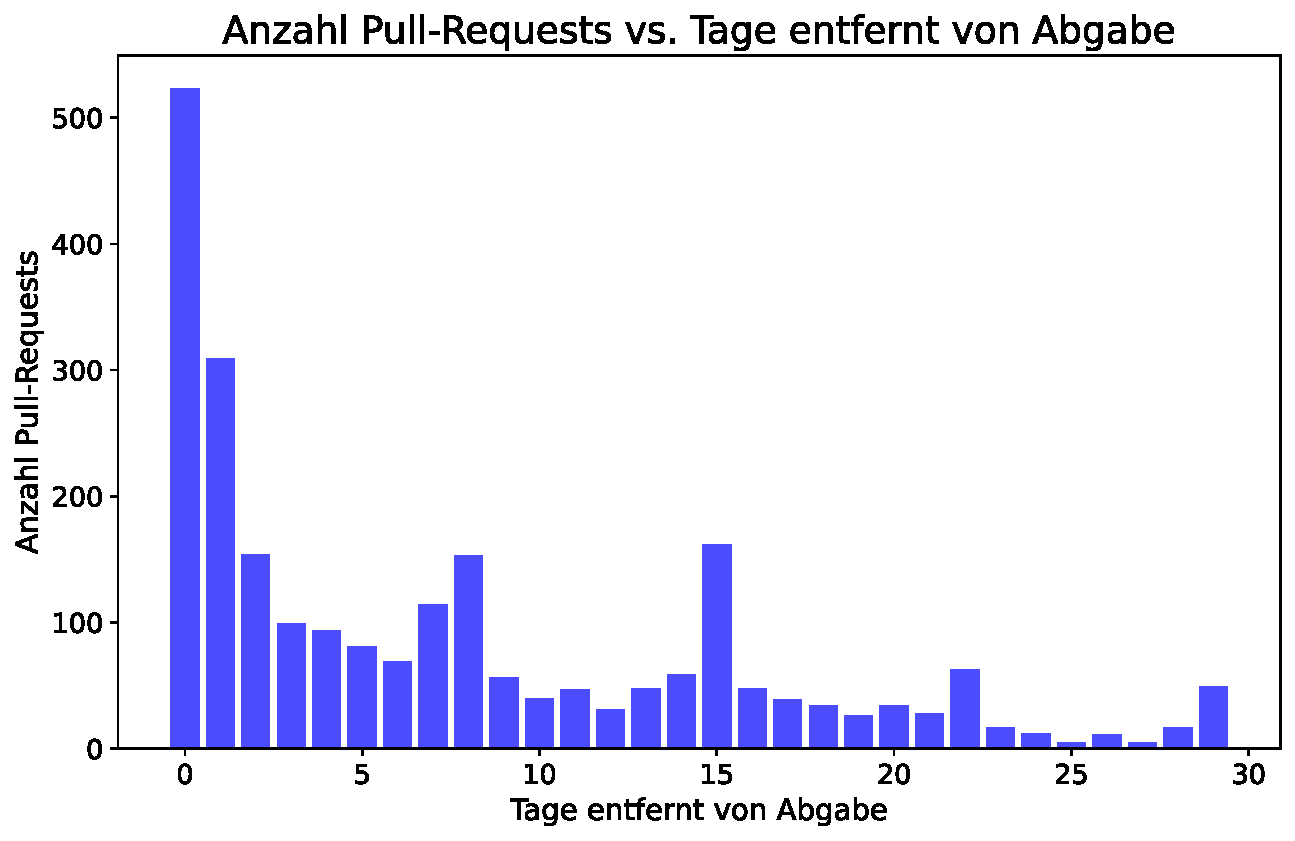
\includegraphics[width=\textwidth]{Figures/anz-prs-days-away-from-end.pdf}
    \caption{Anzahl eröffneter Pull-Requests im Verhältnis zur Abgabe}
    \label{fig:anz-prs-days-away-from-end}
\end{figure}

Eine detaillierte Analyse der Pull-Requests in den einzelnen Teams zeigt, dass in 19 von 71 Teams mehr als 50 Prozent aller Pull-Requests in den letzten drei Projekttagen eröffnet und abgeschlossen wurden. Es lässt sich feststellen, dass vier der analysierten Teams einen Anteil von über 75 Prozent ihrer Pull-Requests in diesem Zeitraum bearbeitet haben. Zudem ist eine Gruppe zu identifizieren, die sämtliche ihrer Pull-Requests innerhalb des definierten Zeitraums erstellt und geschlossen hat. Eine detaillierte Analyse des Projektes ergab, dass die genannte Gruppe insgesamt zwei Pull-Requests hatte, die beide am Tag vor der Abgabe erstellt wurden. Wenn diese Analyse auf den letzten Projekttag beschränkt wird, dann sind es drei Teams, die mehr als 50 Prozent ihrer Pull-Requests am Abgabetag erledigt haben.

Viele Pull-Requests werden gegen Ende der Projekte erstellt und wie im Kapitel \secref{sec:ProjektwochenLatencyChurn} aufgezeigt, nehmen die Latencies gegen Ende der Projekte ab. Jedoch ist dort nicht genau ersichtlich, wie dies bei den einzelnen Projekten aussieht. Deshalb werden die Latencies unter 30 Minuten und die ganz kurzen Latencies von unter einer Minute im Verhältnis zu den Abgaben gestellt.

\subsection{Analyse kurze Pull-Request-Latency im Verhältnis zur Abgabe }
Eine detaillierte Analyse der kurz geöffneten Pull-Requests (unter 30 Minuten) offenbart, dass der überwiegende Teil davon in den letzten drei Tagen und insbesondere am Tag der Abgabe erstellt wird. Eine weitere Restriktion der Pull-Requests auf jene, die innerhalb einer Minute abgearbeitet werden, resultiert in einer ähnlichen Situation. Es ist jedoch festzustellen, dass der Tag der Abgabe sich stärker abhebt, wobei auch ein Anstieg zwei Tage vor Abgabe zu erkennen ist.  Die Resultate sind in \autoref{fig:anz-prs-under-x-mins} dargestellt.

\begin{figure}[htbp]
    \centering
    \begin{subfigure}[b]{0.48\textwidth}
        \centering
        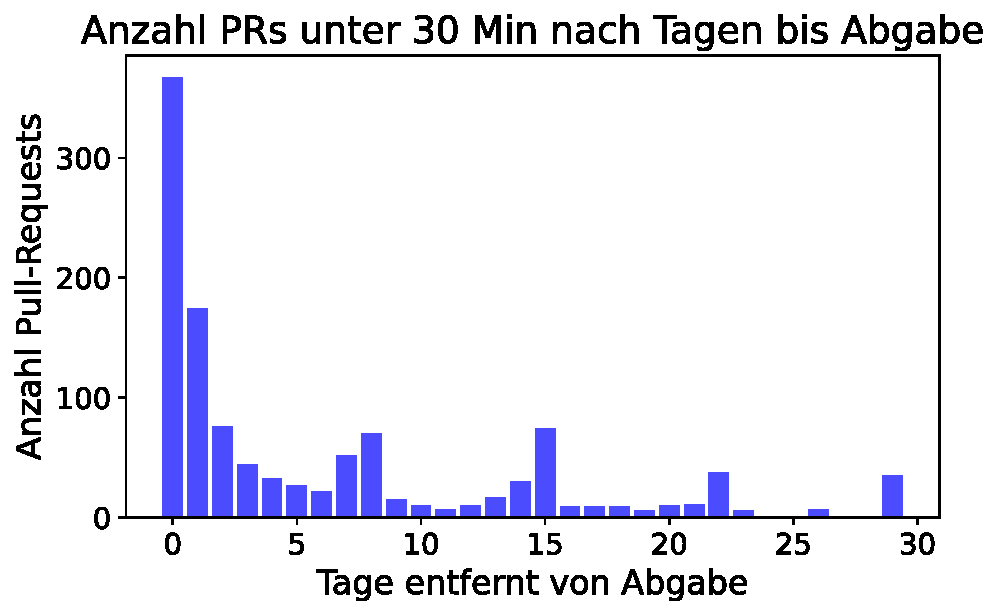
\includegraphics[width=\textwidth]{Figures/anz-prs-under-30-min.pdf}
    \caption{Anzahl Pull-Requests unter 30 Minuten im Verhältnis zur Abgabe}
    \label{fig:anz-prs-under-30-min}
    \end{subfigure}
    \hfill
    \begin{subfigure}[b]{0.48\textwidth}
        \centering
        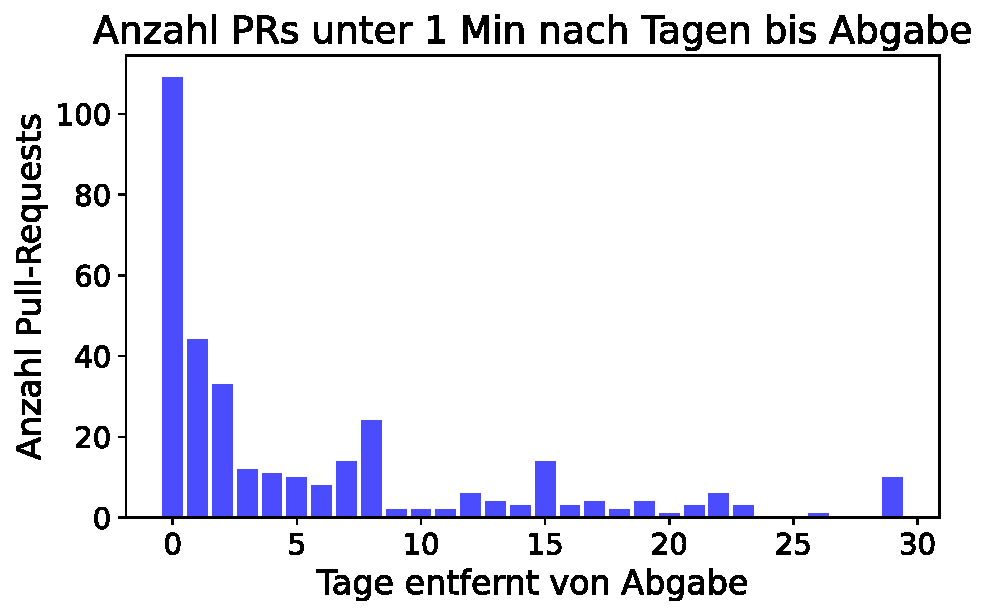
\includegraphics[width=\textwidth]{Figures/anz-prs-under-1-min.pdf}
    \caption{Anzahl Pull-Requests unter einer Minute im Verhältnis zur Abgabe}
    \label{fig:anz-prs-under-1-min}
    \end{subfigure}
    \caption{Anzahl Pull-Requests unter 30 / 1 Minute im Verhältnis zur Abgabe}
    \label{fig:anz-prs-under-x-mins}
\end{figure}

\subsection{Zusammenfassung}
Die Analyse zeigt deutlich, dass die Bearbeitungszeit von Pull-Requests im Verlauf der Projektlaufzeit stark abnimmt, besonders in den letzten drei Tagen vor Abgabe. Gleichzeitig nimmt der Churn bis zur letzten Projektwoche kontinuierlich zu.

Über 40\,\% aller Pull-Requests werden in den letzten drei Tagen der Projekte erstellt und abgeschlossen, wobei am Tag der Abgabe die meisten Pull-Requests erstellt werden. Dies zeigt sich auch an der erhöhten Anzahl von Pull-Requests mit besonders kurzen Bearbeitungszeiten (unter 30 Minuten und unter einer Minute) am Abgabetag.

Ein Vergleich zwischen den Vollzeit- und Teilzeitklassen zeigt, dass die Vollzeitklassen besonders in der ersten Projektwoche längere Bearbeitungszeiten besitzen als die Teilzeitklassen. Der Churn zeigt bei beiden Gruppen ein ähnliches Verhalten über den gesamten Projektverlauf.

Zusätzlich wurde festgestellt, dass die Gesamtzahl der Pull-Requests in der ersten Projektwoche am niedrigsten ist, danach kontinuierlich bis zur vierten Woche ansteigt und in der fünften Woche leicht abnimmt. Wenige Pull-Requests wurden in einer sechsten Projektwoche erstellt, da nur noch wenige Projekte zu diesem Zeitpunkt aktiv waren.

Die durchgeführten Analysen stellen einen wie in der \fref{forschungsfrage3} gestellten Zusammenhang fest. Die Review-Zeiten für Pull-Requests nehmen gegen Ende der Projekte stark ab, insbesondere in den letzten Tagen der Projekte.

%----------------------------------------------------------------------------------------
% SECTION 4
%----------------------------------------------------------------------------------------

\section{Ergebnisse Entwicklungs\-aktivi\-tät}
\label{sec:ErgebnisseEntwicklungsaktivtät}
Empirische Studien zeigen, dass die Entwicklungsaktivität in Open-Source-Projek\-ten auf Plattformen wie GitHub charakteristische Muster im Wochenverlauf aufweist. Insbesondere an Wochenenden ist die Aktivität signifikant geringer als unter der Woche. Innerhalb der Arbeitswoche fallen Montag und Freitag häufig als die Tage mit der geringsten Aktivität auf. Das Phänomen des Rückgangs der Entwicklungsaktivität wird oftmals auch Friday Effect genannt. \parencite{claes_programmers_2018}

Dies soll nun im Zusammenhang mit der \fref{forschungsfrage4} "\textit{Lassen sich Patterns der Zusammenarbeit im Team erkennen,
hinsichtlich der Tage, an denen die Studierenden an den Projekten arbeiten?}" anhand der Projektmodule analysiert werden. Um diese Analyse durchführen zu können, werden die Klassen einzeln nach ihren Arbeitstagen analysiert. Die Arbeitstage werden anhand der offenen und geschlossenen Pull-Requests und der Commit-Daten definiert. Für dies wird das Mining um die im Kapitel \secref{sec:Metriken} erwähnte Metrik commit ergänzt.

Um die Entwicklungsaktivität messbar machen zu können, mussten für alle Klassen die Projektmodul-Unterrichtstage nachgeschlagen werden. Diese sind in \autoref{tab:stundenplan} ersichtlich. 
\begin{table}[ht]
\caption{Projektmodul-Unterrichtstage der Klassen}
\label{tab:stundenplan}
\centering
\begin{tabular}{l l l}
\toprule
\textbf{Klasse} & \textbf{Ort} & \textbf{Tag} \\
\midrule
It21tb   & Zürich      & Montag      \\
It21ta   & Zürich      & Montag      \\
It21a    & Zürich      & Mittwoch    \\
It21tb   & Winterthur  & Donnerstag  \\
It21a    & Winterthur  & Freitag     \\
It21b    & Winterthur  & Freitag     \\
It21ta   & Winterthur  & Freitag     \\
\midrule
It23tb   & Zürich      & Montag      \\
It23ta   & Zürich      & Montag      \\
It23a    & Zürich      & Mittwoch    \\
It23b    & Zürich      & Mittwoch    \\
It23a    & Winterthur  & Freitag     \\
It23ta   & Winterthur  & Freitag     \\
It23tb   & Winterthur  & Freitag     \\
\midrule
It24tb   & Zürich      & Montag      \\
It24ta   & Zürich      & Montag      \\
It24a    & Zürich      & Mittwoch    \\
It24a    & Winterthur  & Freitag     \\
It24ta   & Winterthur  & Freitag     \\
It24tb   & Winterthur  & Freitag     \\
\bottomrule
\end{tabular}
\end{table}


Da sich während der Analyse  Differenzen zwischen den Voll- und Teilzeitklassen ergaben, werden diese getrennt angeschaut. 

\subsection{Arbeitstage Pull-Requests}
Als Erstes werden die Wochentage der Pull-Request-Erstellungs- und Schliessungsdaten ermittelt und auf die Wochentage aufgeteilt. Diese Aufteilung wird pro Klasse vorgenommen. In den vorliegenden Daten zeigt sich eine Tendenz zur Konzentration der Aktivitäten auf spezifische Wochentage, insbesondere auf die jeweiligen Unterrichtstage. So wurden bei den Vollzeitklassen rund 24\,\% aller Pull-Requests am Projekttag erstellt. Bei den Teilzeitklassen liegt dieser Wert mit 34\,\% deutlich höher. Dies unterstreicht die Bedeutung des Unterrichtstages für die praktische Arbeit im Rahmen des Projekts.

Die \autoref{fig:anz-prs-teilzeit-pro-wochentag} zeigt exemplarisch die Verteilung der PR-Erstellungen auf die Wochentage für zwei Teilzeitklassen. Deutlich erkennbar ist eine Aktivitätsspitze am jeweiligen Unterrichtstag. An den folgenden Tagen nimmt die Aktivität deutlich ab. Auffällig ist auch, dass am Unterrichtstag nicht nur PRs erstellt, sondern auch überprüft und geschlossen wurden. Insgesamt ist der Anteil der am Wochenende erstellten PRs mit 27.7\,\% vergleichsweise hoch.

\begin{figure}[htbp]
    \centering
    \begin{subfigure}[b]{0.48\textwidth}
        \centering
        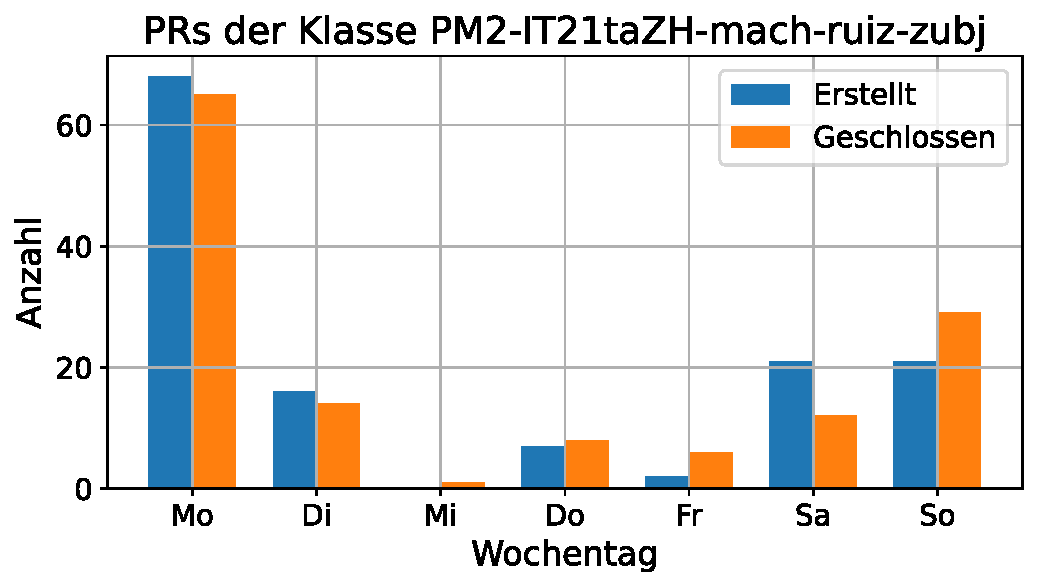
\includegraphics[width=\textwidth]{Figures/pr-klasse-per-wochentag-it21ta.pdf}
         \caption{Anzahl geöffneter PRs pro Wochentag der Teilzeitklasse It21ta (Unterrichtstag Montag)}
        \label{fig:anzahl-prs-pro-wochentag-it21ta}
    \end{subfigure}
    \hfill
    \begin{subfigure}[b]{0.48\textwidth}
        \centering
        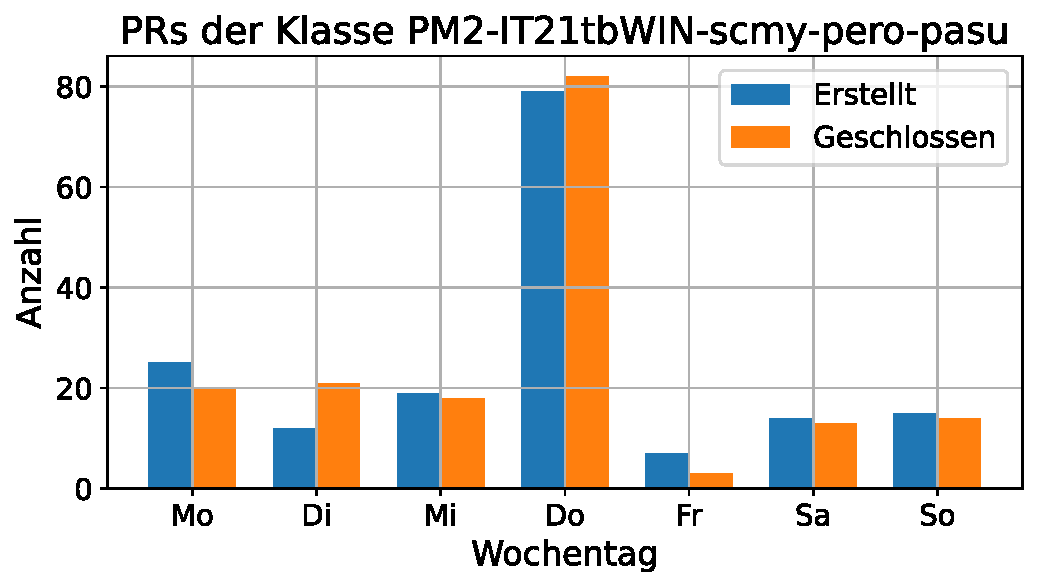
\includegraphics[width=\textwidth]{Figures/pr-klasse-per-wochentag-21tb.pdf}
         \caption{Anzahl geöffneter PRs pro Wochentag der Teilzeitklasse It21tb (Unterrichtstag Donnerstag)}
        \label{fig:anzahl-prs-pro-wochentag-it21tb}
    \end{subfigure}
    \caption{Anzahl geöffneter PRs pro Wochentag von 2 Teilzeitklassen}
    \label{fig:anz-prs-teilzeit-pro-wochentag}
\end{figure}

Ein gegensätzliches Bild zeigt sich bei den Vollzeitklassen. Die \autoref{fig:anz-prs-vollzeit-pro-wochentag} zeigt die Verteilung der PR-Erstellungen und Schliessungen für zwei exemplarische Klassen.
Hier zeigt sich eine insgesamt gleichmässigere Verteilung der Aktivitäten über die Woche. Zwar ist auch hier der Projekttag am aktivsten, jedoch meist in geringerem Ausmass als bei den Teilzeitklassen. Zudem wurden nur 16.8\,\% der PR am Wochenende erstellt.

\begin{figure}[htbp]
    \centering
    \begin{subfigure}[b]{0.48\textwidth}
        \centering
        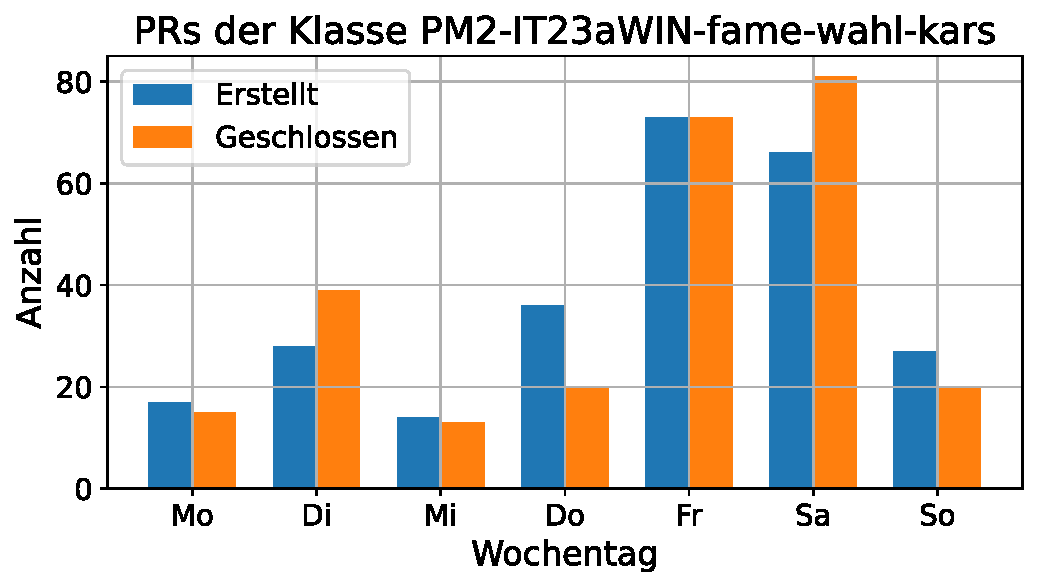
\includegraphics[width=\textwidth]{Figures/pr-klasse-per-wochentag-23a.pdf}
         \caption{Anzahl geöffneter PRs pro Wochentag der Vollzeitklasse It23a (Unterrichtstag Freitag)}
        \label{fig:anzahl-prs-pro-wochentag-it23a}
    \end{subfigure}
    \hfill
    \begin{subfigure}[b]{0.48\textwidth}
        \centering
        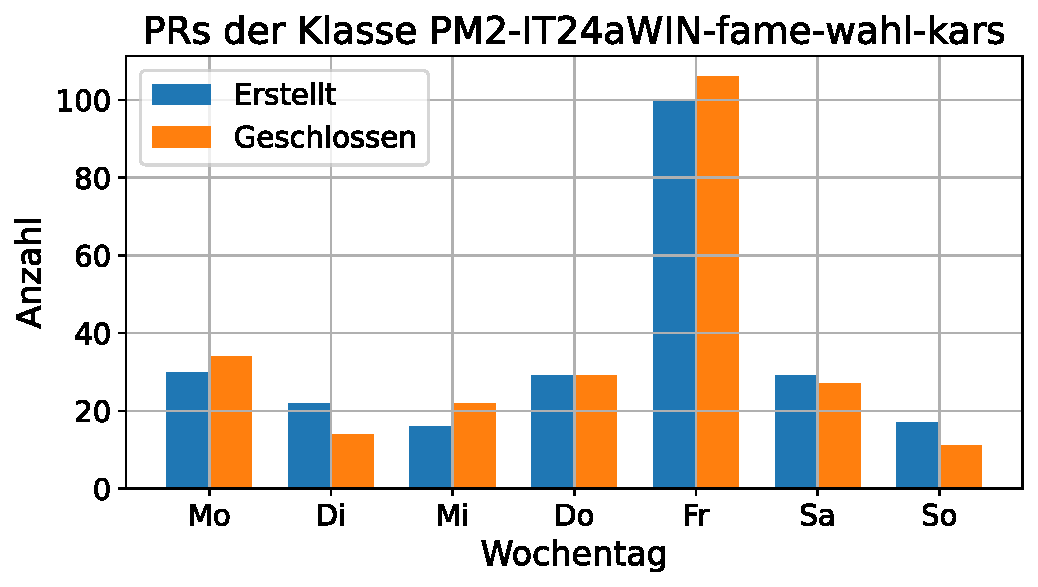
\includegraphics[width=\textwidth]{Figures/pr-klasse-per-wochentag-24a.pdf}
         \caption{Anzahl geöffneter PRs pro Wochentag der Vollzeitklasse It24a (Unterrichtstag Freitag)}
        \label{fig:anzahl-prs-pro-wochentag-it24a}
    \end{subfigure}
    \caption{Anzahl geöffneter PRs pro Wochentag von 2 Vollzeitklassen}
    \label{fig:anz-prs-vollzeit-pro-wochentag}
\end{figure}


\subsection{Arbeitstage Commits}
Da sowohl die PRs als auch die einzelnen Commits für die Entwicklungsanalyse von Interesse sind, wurden die Commits der PRs analysiert.
Die Analyse bestätigt die in der PR-Analyse bereits festgestellten Ergebnisse.

So wurden bei den Vollzeitklassen 23.7\,\% aller Commits am jeweiligen Unterrichtstag durchgeführt. Bei den Teilzeitklassen liegt dieser Anteil mit 33.9\,\% deutlich höher. Die \autoref{fig:anz-commits-teilzeit-pro-wochentag} zeigt die Verteilung der Commits über die Wochentage exemplarisch für zwei Teilzeitklassen. Analog zur PR-Verteilung ist eine deutliche Spitze an den jeweiligen Projekttagen erkennbar. Insgesamt wurden 25.9\,\% aller Commits der Teilzeitklassen an einem Samstag oder Sonntag durchgeführt.

\begin{figure}[htbp]
    \centering
    \begin{subfigure}[b]{0.48\textwidth}
        \centering
        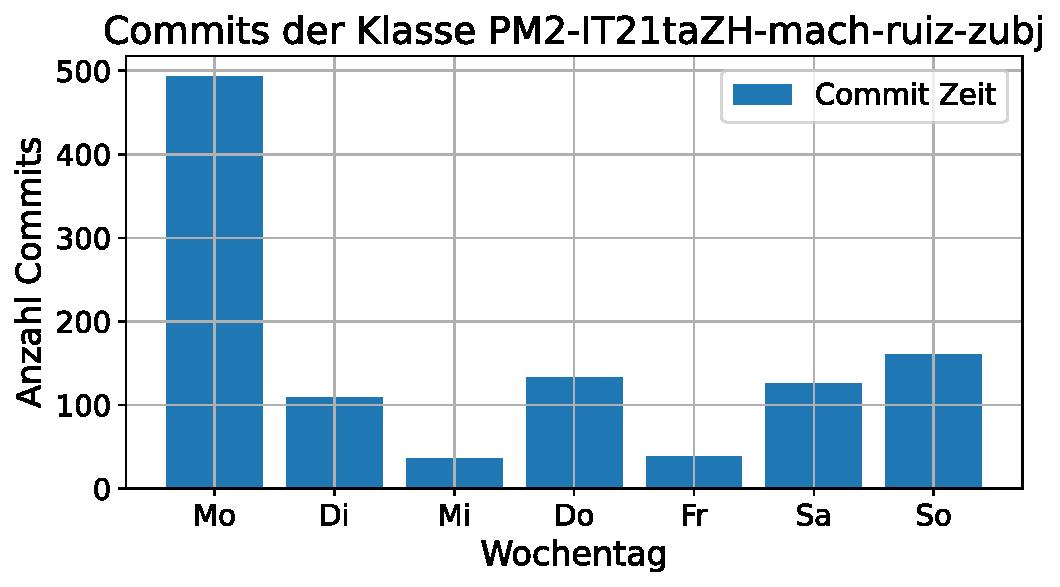
\includegraphics[width=\textwidth]{Figures/commits-klasse-per-wochentag-21ta.pdf}
         \caption{Anzahl Commits pro Wochentag der Teilzeitklasse It21ta (Unterrichtstag Montag)}
        \label{fig:anzahl-commits-pro-wochentag-it21ta}
    \end{subfigure}
    \hfill
    \begin{subfigure}[b]{0.48\textwidth}
        \centering
        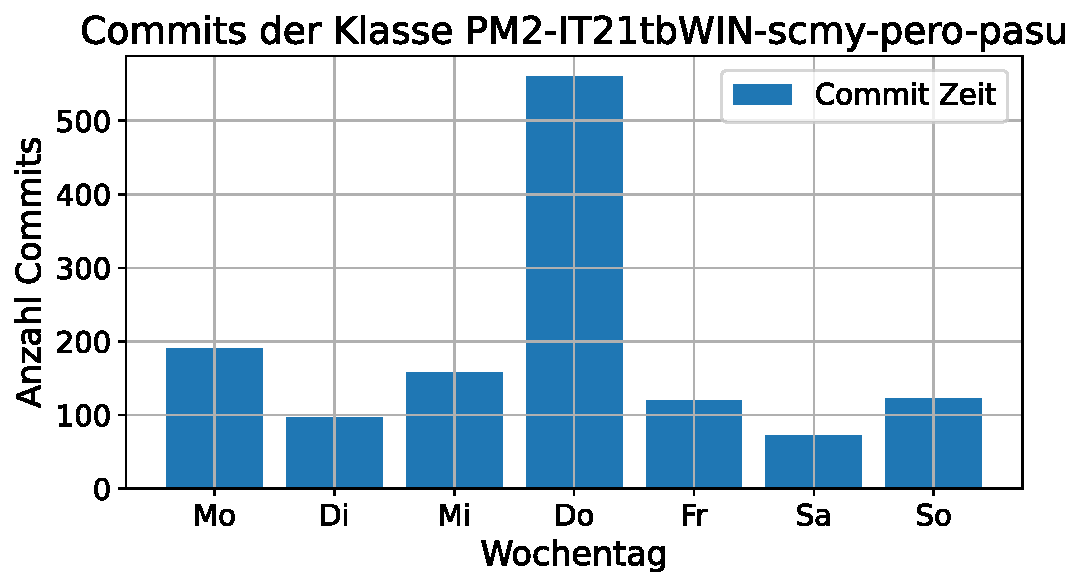
\includegraphics[width=\textwidth]{Figures/commits-klasse-per-wochentag-21tb.pdf}
         \caption{Anzahl Commits pro Wochentag der Teilzeitklasse It21tb (Unterrichtstag Donnerstag)}
        \label{fig:anzahl-commits-pro-wochentag-it21tb}
    \end{subfigure}
    \caption{Anzahl Commits pro Wochentag von 2 Teilzeitklassen}
    \label{fig:anz-commits-teilzeit-pro-wochentag}
\end{figure}

Ein ähnliches Bild ergibt sich auch bei den Vollzeitklassen zwischen Pull-Requests und Commits. Die \autoref{fig:anz-commits-vollzeit-pro-wochentag} zeigt die Commits zweier exemplarischer Klassen. Hier wurden 23.7\,\% der Commits am jeweiligen Projekttag durchgeführt, was dem PR-Anteil entspricht. Am Wochenende hingegen wurden nur 19.4\,\% der Commits verzeichnet, was deutlich unter dem Wert der Teilzeitklassen liegt.

\begin{figure}[htbp]
    \centering
    \begin{subfigure}[b]{0.48\textwidth}
        \centering
        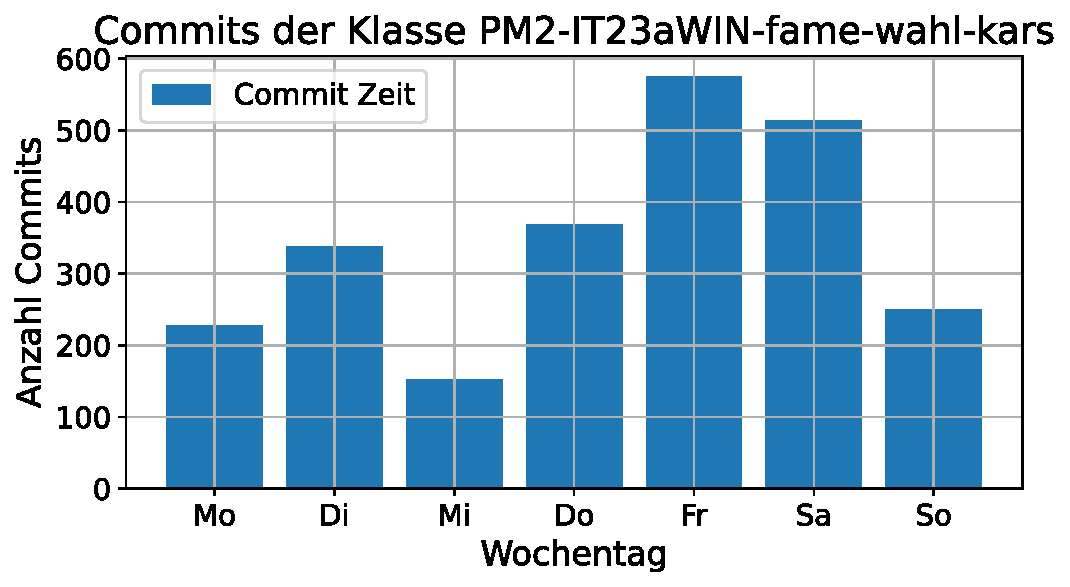
\includegraphics[width=\textwidth]{Figures/commits-klasse-per-wochentag-23a.pdf}
         \caption{Anzahl Commits pro Wochentag der Vollzeitklasse It23a (Unterrichtstag Freitag)}
        \label{fig:anzahl-commits-pro-wochentag-it23a}
    \end{subfigure}
    \hfill
    \begin{subfigure}[b]{0.48\textwidth}
        \centering
        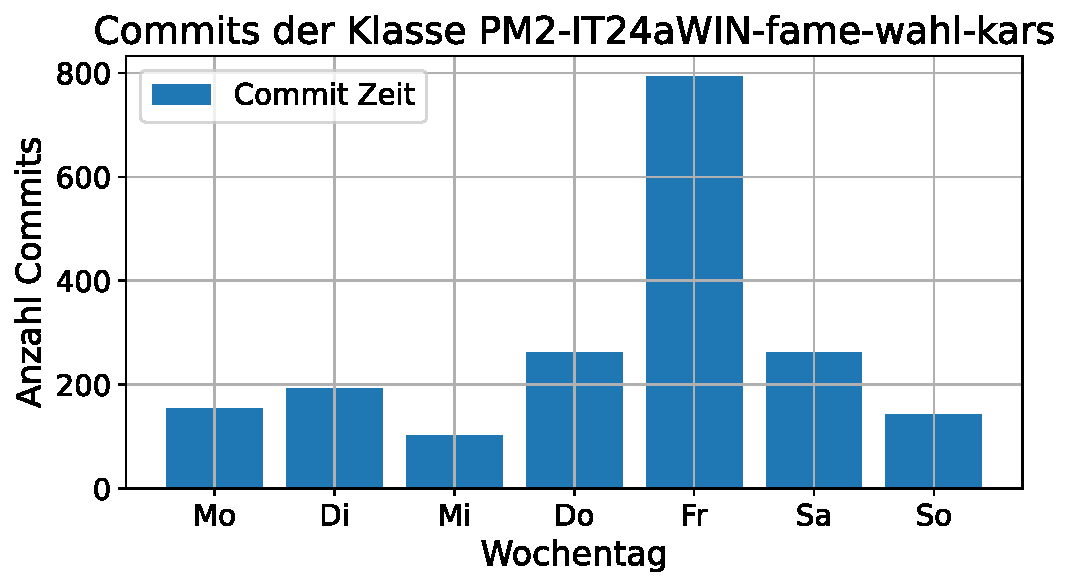
\includegraphics[width=\textwidth]{Figures/commits-klasse-per-wochentag-24a.pdf}
         \caption{Anzahl Commits pro Wochentag der Vollzeitklasse It24a (Unterrichtstag Freitag)}
        \label{fig:anzahl-commits-pro-wochentag-it24a}
    \end{subfigure}
    \caption{Anzahl Commits pro Wochentag von 2 Vollzeitklassen}
    \label{fig:anz-commits-vollzeit-pro-wochentag}
\end{figure}


\subsection{Zusammenfassung}
Die Analyse zeigt deutlich, dass die Entwicklungsaktivität stark vom Unterrichtstag der Klassen beeinflusst wird. Sowohl bei den Pull-Requests als auch bei den Commits zeigt sich eine Konzentration der Aktivitäten auf den jeweiligen Projekttag, wobei dieser Effekt bei den Teilzeitklassen deutlicher ausgeprägt ist als bei den Vollzeitklassen.

Bei den Teilzeitklassen wurden etwa 34\,\% aller Pull-Requests und Commits am Unterrichtstag durchgeführt. Zudem ist bei diesen Klassen die Aktivität am Wochenende mit rund 28\,\% der Pull-Requests und 26\,\% der Commits relativ hoch. Die Vollzeitklassen zeigen ein gleichmässigeres Aktivitätsmuster über die Wochentage verteilt, mit ungefähr 24\,\% der Pull-Requests und Commits am Projekttag und einer niedrigeren Wochenendaktivität von etwa 17\,\% (Pull-Requests) bzw. 19\,\% (Commits).

Zusammenfassend kann zur \fref{forschungsfrage4} festgestellt werden, dass klare Patterns der Zusammenarbeit innerhalb der Teams bestehen, insbesondere hinsichtlich einer verstärkten Aktivität am jeweiligen Unterrichtstag sowie einer signifikant höheren Wochenendaktivität bei den Teilzeitklassen im Vergleich zu den Vollzeitklassen.
Diese Unterschiede in den Arbeitsrhythmen der beiden Unterrichtsmodelle zeigen, dass Dozierende auf unterschiedliche Rahmenbedingungen treffen, die bei der Betreuung und Bewertung der Projekte unbedingt berücksichtigt werden sollten.
%----------------------------------------------------------------------------------------
% SECTION 5
%----------------------------------------------------------------------------------------
\section{Unterschiede von Teilzeitstudierenden und Vollzeitstudierenden in der Pull-Request-Nutzung}
Zur detaillierten Analyse der \fref{forschungsfrage5} "\textit{Welche Unterschiede zeigen sich in der Nutzung von Pull-Requests zwischen Teilzeit- und Vollzeitstudierenden hinsichtlich Anzahl, Umfang und Dauer?}" erfolgt eine Aufteilung der Repository-Daten auf Teilzeit- und Vollzeitklassen. Die Anzahl der Pull-Requests der Teilzeitklassen beläuft sich auf 1'369 und jene der Vollzeitklassen auf 1'066. Dabei werden durchschnittlich 31.8 Pull-Requests von den Teilzeitstudierenden erstellt und 39.5 von den Vollzeitstudierenden. Die wichtigsten Kennzahlen sind in \autoref{tab:deskriptive-kennzahlen-teilzeit-vollzeit} aufgezeigt.

\begin{table}[htbp]
    \centering
    \caption{Kennzahlen zu Latency und Churn von Teilzeit- und Vollzeitklassen}
    \begin{tabular}{@{}lrrrr@{}}
        \toprule
        \makecell{}&
        \makecell{\textbf{Latency (Std.)} \\ \textbf{Teilzeit}}&
        \makecell{\textbf{Latency (Std.)} \\ \textbf{Vollzeit}}&
        \makecell{\textbf{Churn} \\ \textbf{Teilzeit}}&
        \makecell{\textbf{Churn} \\ \textbf{Vollzeit}}\\
        \midrule
        Mittelwert & 19.9 & 16.9 & 260.2 & 301.3 \\
        Standardabweichung &  47.2 & 34.2  & 678.1 & 964.1 \\
        Minimum & 0.0008 & 0.001 & 0.0 & 0.0 \\
        1. Quartil (Q1) & 0.04 & 0.07 & 27.0 & 28.3\\
        Median & 0.5 & 0.8 & 93.0 & 97.0 \\
        3. Quartil (Q3) &  15.1 & 17.5 & 249.0 & 254.5 \\
        Maximum & 416.3 & 265.0 & 13'206.0 & 17'299.0 \\
        \bottomrule
    \end{tabular}
    \label{tab:deskriptive-kennzahlen-teilzeit-vollzeit}
\end{table}


\subsection{Deskriptive Analyse der Metriken}
Die latency zeigt, dass Teilzeitstudierende im Durchschnitt mehr Zeit benötigen, um einen PR zu bearbeiten. Der Median zeigt jedoch, dass Teilzeitstudierende häufiger sehr kurze Pull-Request-Latencies haben. Dabei ist bei beiden die Bearbeitungszeit im Median deutlich kürzer. Ausserdem ist zu erkennen, dass die Teilzeitstudierenden eine grössere Streuung der Bearbeitungszeiten aufweisen. Sie haben also einige Pull-Requests, die deutlich länger dauern. Dies ist auch im Maximum zu sehen, welches bei den Teilzeitstudierenden bei 416 Stunden liegt, was 17 Tagen entspricht. Wobei die Vollzeitstudierenden ein Maximum von 265 Stunden haben, was 11 Tagen entspricht.

Der Churn zeigt, dass Vollzeitstudierende sowohl im Durchschnitt als auch im Median mehr Zeilenänderungen pro Pull-Request vornehmen. Die Standardabweichung zeigt ebenfalls, dass Vollzeitstudierende grössere Schwankungen in der Anzahl der Zeilenänderungen haben. Im Maximum ist ersichtlich, dass beide sehr grosse PRs haben, wobei sich das Maximum der Vollzeitstudierenden nochmals um mehr als 4'000 Zeilen von dem Maximum der Teilzeitstudierenden unterscheidet.

Auch die Struktur der PRs unterscheidet sich leicht zwischen den Unterrichtsmodellen: Die durchschnittliche Anzahl bearbeiteter Dateien pro PR liegt insgesamt bei 5.66 Dateien. Teilzeitklassen weisen mit 5.85 im Schnitt mehr betroffene Dateien auf als Vollzeitklassen mit 5.42 Dateien. Ebenso zeigt sich bei der durchschnittlichen Anzahl Commits pro PR ein Unterschied: Insgesamt liegt der Durchschnitt bei 7.03 Commits pro PR, wobei Teilzeitklassen auf 6.50 und Vollzeitklassen auf 7.70 Commits pro PR kommen.

\subsection{Verteilung der Latencies}
Um die Verteilung der Latencies zu analysieren, werden die Daten in Intervalle eingeteilt. Die Festlegung dieser Intervalle erfolgt auf der Grundlage bereits analysierter Daten. Nachfolgend eine Liste dieser Intervalle und die Gründe, warum sie so definiert wurden: 

\begin{itemize}
    \item \textbf{[0-1min]}: Für Pull-Requests, die sofort gemerged werden.
    \item \textbf{[1-5min]}: Für Pull-Requests, die schnell gemerged werden, bei denen aber noch genügend Zeit bleibt, sehr kleine Änderungen ernsthaft zu prüfen.
    \item \textbf{[5-30min]}: Für kleinere oder unkomplizierte Änderungen.
    \item \textbf{[0.5-1h]}: Um zu sehen, wie viele innerhalb einer Stunde abgeschlossen werden.
    \item \textbf{[1-4h]}: Diese Abgrenzung wurde gewählt, da 4 Stunden einen halben Arbeitstag / Studientag widerspiegeln, zum Beispiel auch die 4 Lektionen für die Projektmodul-Vorlesung.
    \item \textbf{[4-12h]}: 12 Stunden wurden gewählt, da dies einen halben Tag widerspiegelt, zum Beispiel wenn jemand morgens einen Pull-Request eröffnet und ein Teammitglied abends Zeit hat, diesen zu bearbeiten.
    \item \textbf{[12-24h]}: Für alle Pull-Requests, die innerhalb eines Tages gemerged werden.
    \item \textbf{[1-2d]}: Für alle Pull-Requests, die mit einem Tag Verzögerung gemerged werden.
    \item \textbf{[2-7d]}: Um zu sehen, wie viele Pull-Requests in derselben Woche noch bearbeitet werden.
    \item \textbf{[7d+]}: Für alle Pull-Requests, die länger als eine Woche offen sind.
\end{itemize}


Die \autoref{fig:anz-prs-vs-latency-tv} zeigt die Pull-Requests der Vollzeit- und Teilzeitklassen aufgeteilt in die oben genannten Intervalle. Es ist ersichtlich, dass der Grossteil der Pull-Requests in beiden Unterrichtsmodellen innerhalb der ersten drei Intervalle bearbeitet wurde. Im Intervall [0-1min] heben sich die Klassen der Teilzeitstudierenden jedoch stark ab. 
Die mittleren Latencies von einer halben Stunde bis zu einem Tag sind deutlich geringer. Bei den Unterrichtsmodellen gibt es keine nennenswerten Unterschiede. Lediglich bei den Bearbeitungszeiten von einer bis vier Stunden fallen die Teilzeitstudierenden auf. Auch die Bearbeitungszeiten von einem Tag bis zu einer Woche sind noch gut vertreten. Bei mehr als sieben Tagen heben sich die Teilzeitstudierenden wieder deutlich von den Vollzeitstudierenden ab.

\begin{figure}[htbp]
    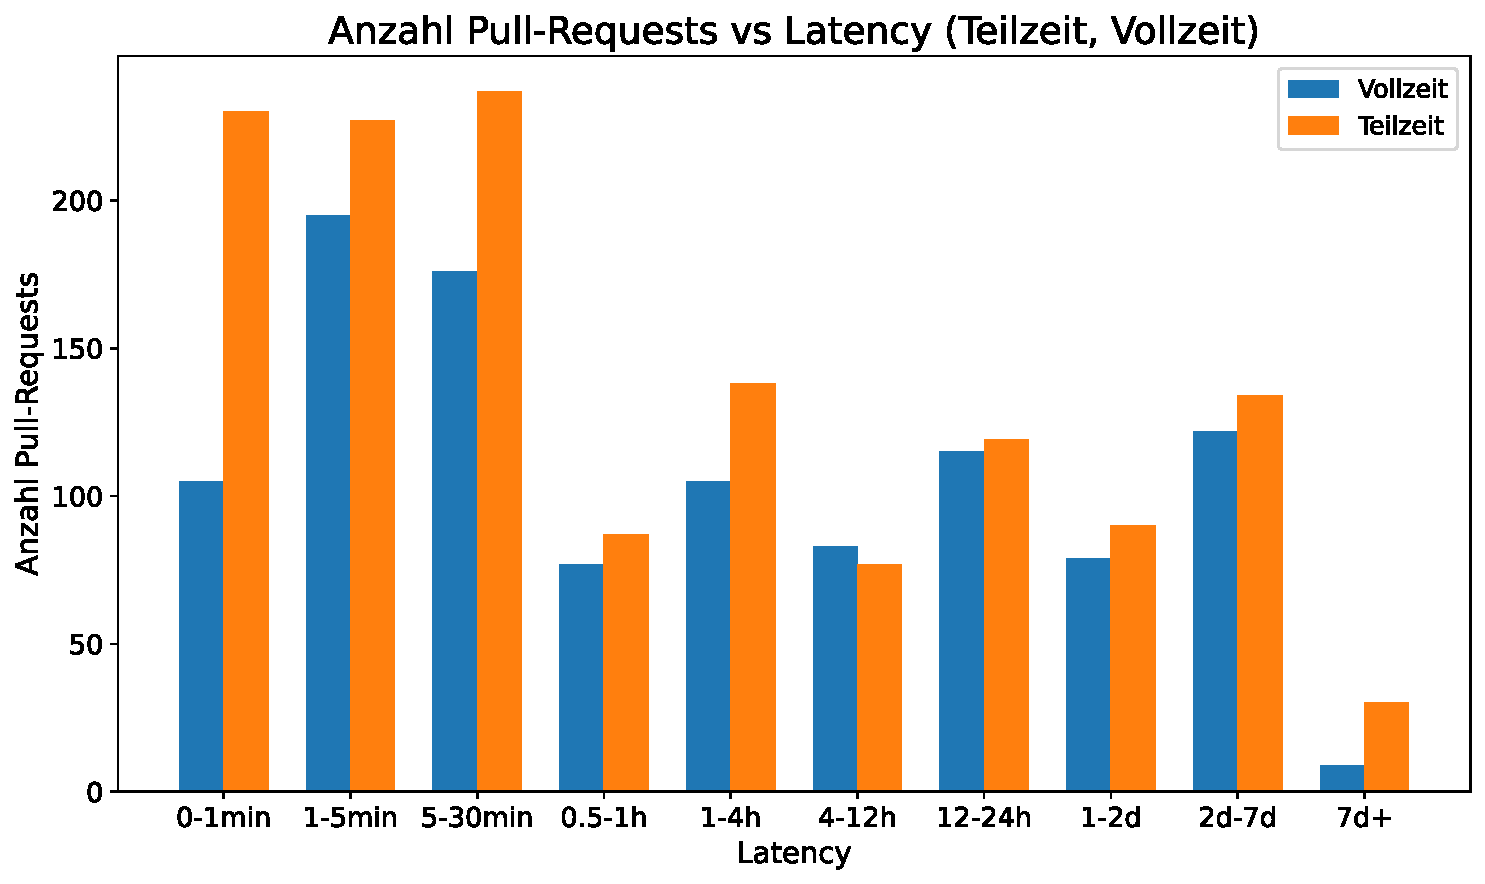
\includegraphics[width=\textwidth]{Figures/anz-prs-vs-latency-tv.pdf}
    \caption{Anzahl Pull-Requests vs. Latency (Teilzeit, Vollzeit)}
    \label{fig:anz-prs-vs-latency-tv}
\end{figure}


Da in der Datenbasis mehr Teilzeitklassen und somit mehr Repositories vorhanden sind, werden die Daten auf die Anzahl der Repositories normiert, was eine unabhängigere Analyse ermöglicht.

Die \autoref{fig:anz-avg-prs-vs-latency-tv} zeigt nun, dass die Teilzeitstudierenden zwar immer noch viele Pull-Requests innerhalb einer halben Stunde bearbeiten, aber nur im ersten Segment die Vollzeitstudierenden übertreffen. In den mittleren Intervallen sind die Teilzeitstudierenden relativ ausgeglichen, aber deutlich weniger als in den ersten drei Intervallen. Bei den Bearbeitungszeiten von mehr als sieben Tagen sind sie jedoch wieder stärker vertreten. Die Vollzeitstudierenden sind über alle Intervalle ausgeglichener, haben aber auch viele schnell bearbeiteten Pull-Requests.


\begin{figure}[htbp]
    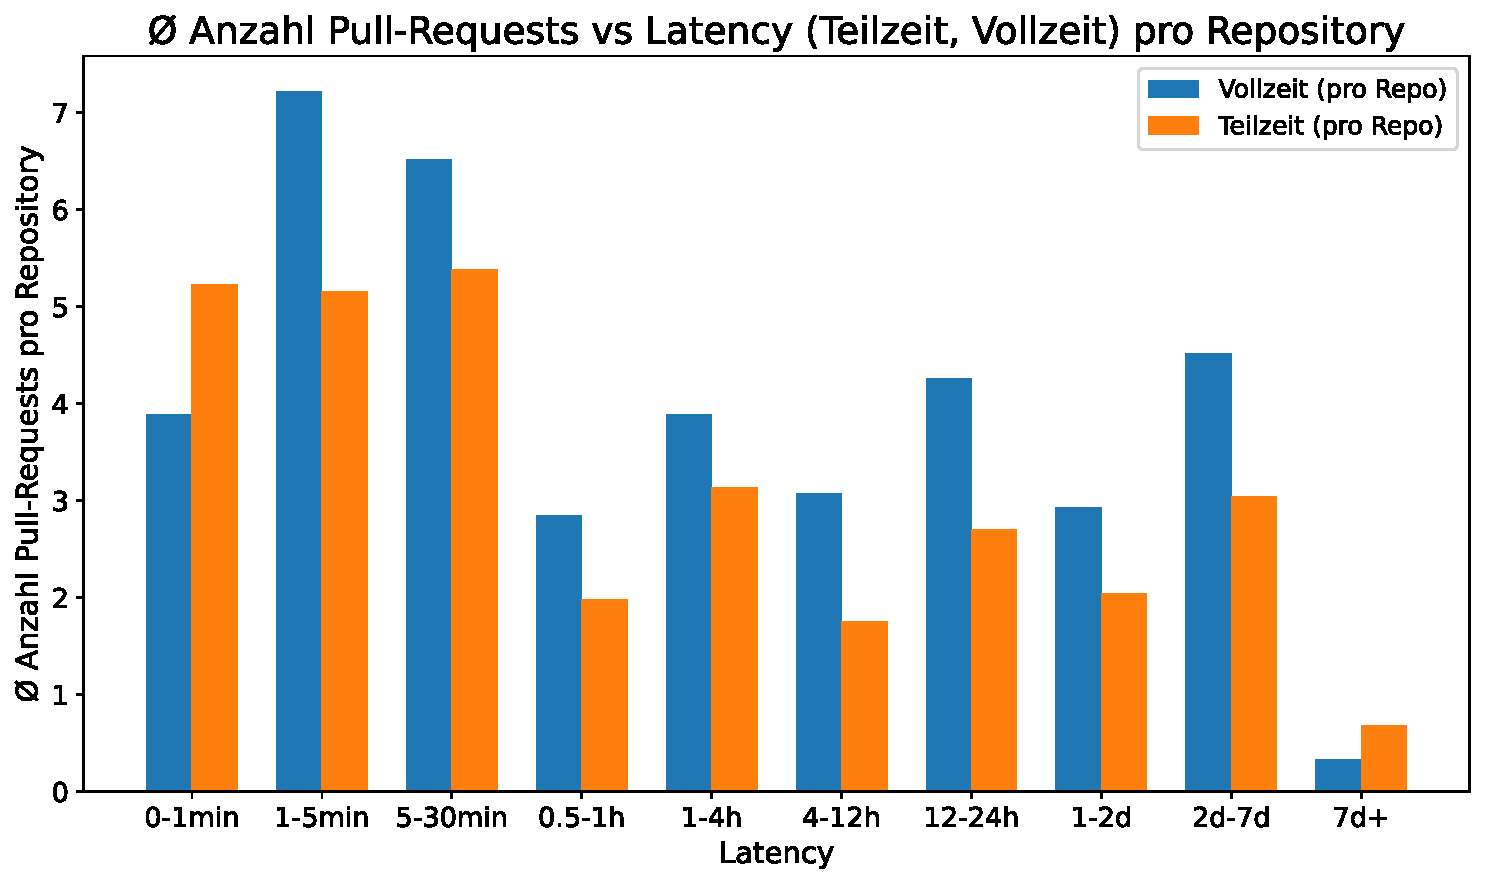
\includegraphics[width=\textwidth]{Figures/anz-avg-prs-vs-latency-tv.pdf}
    \caption{Durchschnittliche Anzahl Pull-Requests vs. Latency (Teilzeit, Vollzeit) pro Repository}
    \label{fig:anz-avg-prs-vs-latency-tv}
\end{figure}


Insgesamt zeigen die Abbildungen \autoref{fig:anz-prs-vs-latency-tv} und \autoref{fig:anz-avg-prs-vs-latency-tv}, dass die meisten Pull-Requests schnell bearbeitet werden. Des Weiteren ist ersichtlich, dass die Teilzeitstudierenden eine stärkere Streuung aufweisen als die Vollzeitstudierenden, da sie die Vollzeitstudierenden im ersten und letzten Intervall übertreffen.

\subsection{Verteilung der Churn-Grössen}
Zur Klassifizierung der Churn-Grösse werden die von Doğan und Tüzün \parencite{dogan_towards_2022} vorgeschlagenen Grössenkategorien (XS, S, M, L, XL) verwendet. Diese Einteilung basiert auf empirischen Studien und industriellen Standards.

Während der manuellen Untersuchung für die \fref{forschungsfrage2} wurde festgestellt, dass einige PRs einen Churn über 10'000 aufweisen. Entweder handelt es sich hierbei um geschlossene PRs, welche entweder aus Versehen oder beispielsweise mit dem falschen Zielbranch erstellt wurden. Um diese klassifizieren zu können, wurde eine zusätzliche Grösse XXL mit Churn 10'000 erstellt. 

Somit ergibt sich für die Analyse die in \autoref{tab:churnkategorien} dargestellte Klassifizierung der Churn-Grössen.
\begin{table}[ht]
\caption{Churn Grössenkategorien}
\label{tab:churnkategorien}
\centering
\begin{tabular}{l l}
\toprule
\textbf{Kategorie} & \textbf{Churn} \\
\midrule
XS  & 0--9       \\
S        & 10--49     \\
M        & 50--199    \\
L         & 200--999   \\
XL   & 1'000--9999 \\
XXL  & 10'000+ \\
\bottomrule
\end{tabular}
\end{table}


Die \autoref{fig:anz-prs-vs-churn-size-tz-vz} zeigt Pull-Requests der Voll- und Teilzeitklassen, aufgeteilt nach ihrer Churn-Grösse. So ist sichtbar, dass die Teilzeitklassen insgesamt mehr PRs erstellen. Dieser Trend ist in allen Grössenkategorien sichtbar, ausser bei den XXL PRs. Hier verfügen die Teilzeitklassen  über 2 PRs, während die Vollzeitklassen 5 PRs mit einem Churn über 10'000 verfügen. Bei den XXS PRs verfügen die Teilzeitklassen über 1.5 Mal so viele PRs.

\begin{figure}[htbp]
    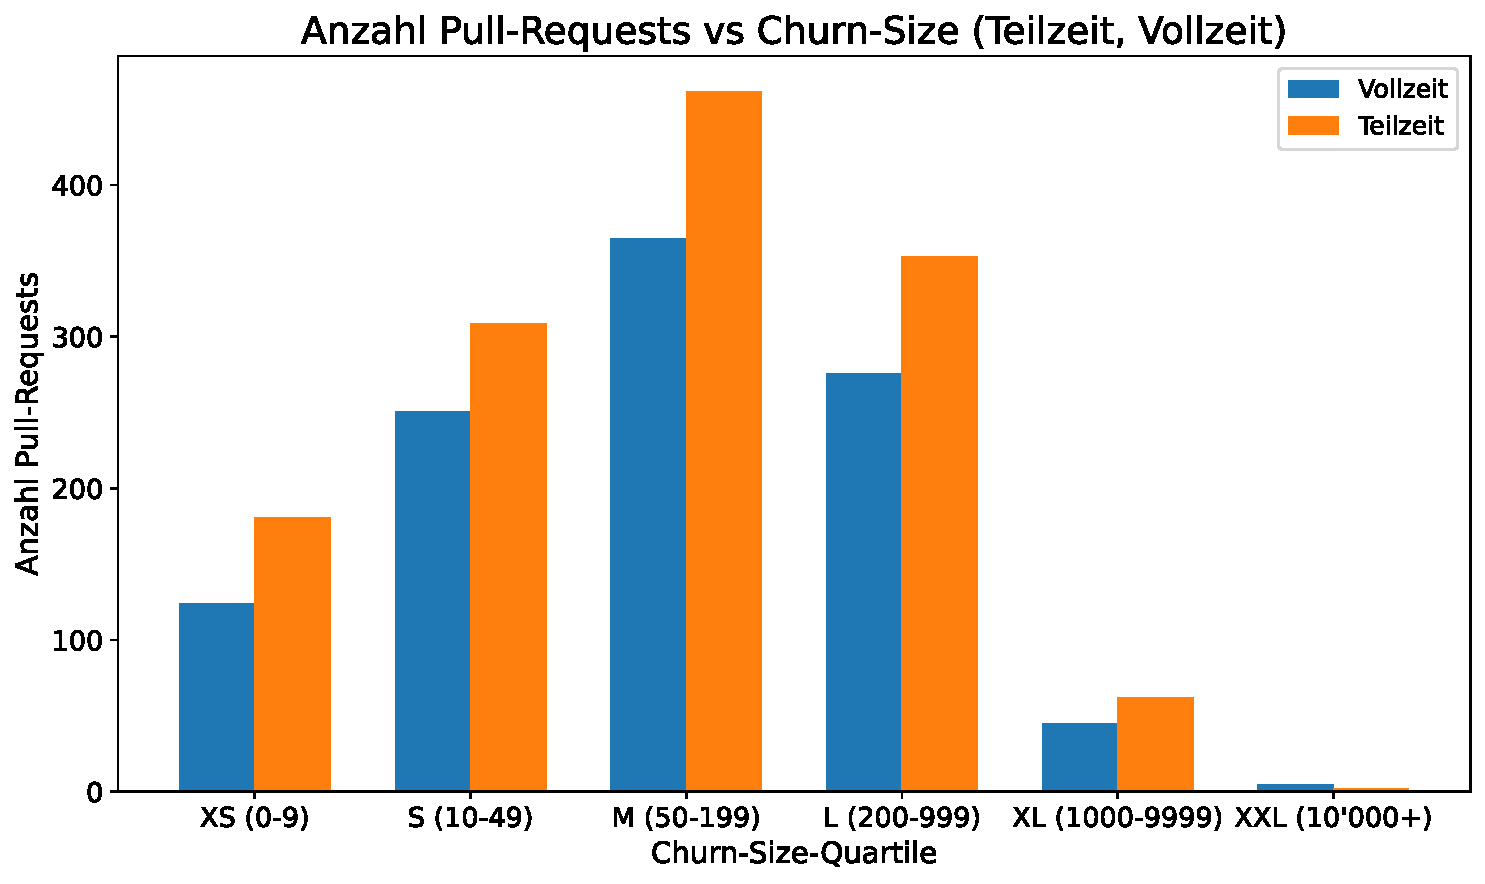
\includegraphics[width=\textwidth]{Figures/anz-prs-vs-churn-size-tz-vz.pdf}
    \caption{Anzahl Pull-Requests vs. Churn-Grösse (Teilzeit, Vollzeit)}
    \label{fig:anz-prs-vs-churn-size-tz-vz}
\end{figure}

Eine Normalisierung der Daten, die nun die durchschnittliche Anzahl der Pull-Requests pro Repository abbildet, ist in \autoref{fig:avg-anz-prs-vs-churn-size-tz-vz-pro-repo} dargestellt. Dabei zeigt sich, dass die Vollzeitklassen in allen Kategorien entweder gleich viele oder mehr Pull-Requests erstellen als die Teilzeitklassen. Die Teilzeitklassen erstellen jedoch fast gleich viele PRs in den Kategorien XS und XL, dort erstellen die Vollzeitklassen jeweils 1.12 und 1.18 so viele PRs. 

\begin{figure}[htbp]
    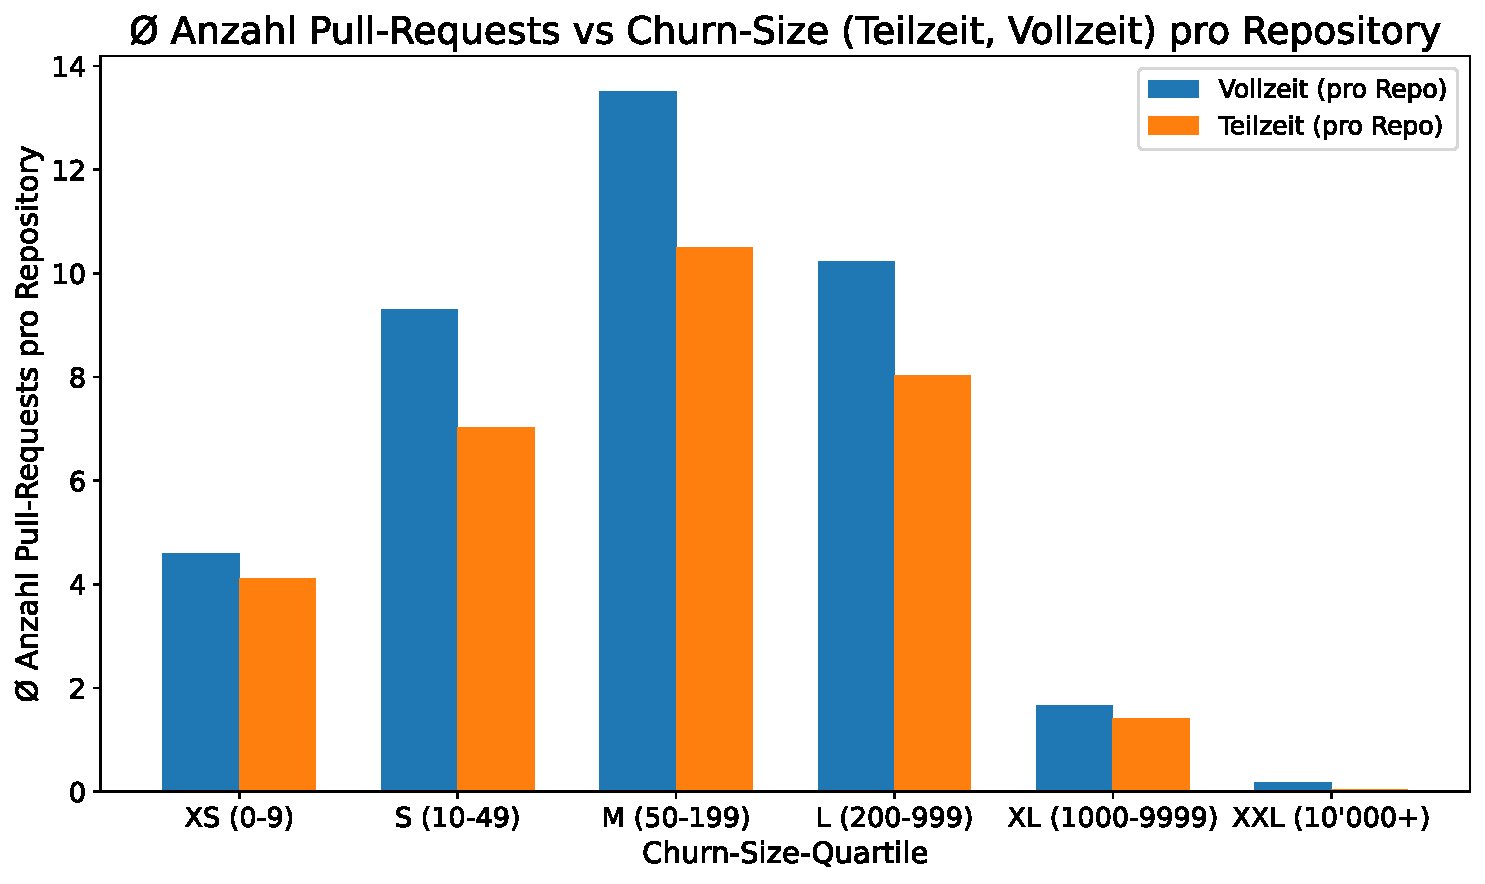
\includegraphics[width=\textwidth]{Figures/avg-anz-prs-vs-churn-size-tz-vz-pro-repo.pdf}
    \caption{Durchschnittliche Anzahl Pull-Requests vs. Churn-Grösse (Teilzeit, Vollzeit) pro Repository}
    \label{fig:avg-anz-prs-vs-churn-size-tz-vz-pro-repo}
\end{figure}


\subsection{Einfluss des Git Flow Branching-Konzept}
Die für die \fref{forschungsfrage2} benötigte manuelle Untersuchung ergab, dass in einigen Klassen das in Kapitel \secref{sec:GitFlow} eingeführte Branching-Konzept Git Flow verwendet wurde. Dies verfälscht eventuell die Daten, da es sich bei den manuell untersuchten Pull-Requests um grosse PRs (Churn) handelt, welche keinen Review erfordern. Aus diesem Grund werden die Analysen erneut durchgeführt, jedoch mit herausgefilterten Dev-Branches.

Da die Namen der Dev-Branches nicht einheitlich sind, werden alle Branches herausgefiltert, die das Wort Dev enthalten und auf den Main/Master Branch gemerged wurden. Dabei ist zu beachten, dass GitHub den heutigen Haupt-Branch Main nennt, während dieser früher Master hiess. In der manuellen Analyse wurde festgestellt, dass einige Klassen aus dem Jahr 2021 immer noch solche Master-Branches verwenden. Zusätzlich wurden alle herausgefilterten Pull-Requests überprüft, um sicherzustellen, dass ausschliesslich Dev-Branches entfernt werden. Es wurden 75 Pull-Requests von Dev-Branches zu Main-Branches ermittelt.


Die \autoref{fig:anz-avg-prs-vs-latency-tv-no-dev} zeigt kaum Differenzen zur \autoref{fig:anz-avg-prs-vs-latency-tv}. Generell hat die durchschnittliche Anzahl der Pull-Requests abgenommen, aber die Verteilung der Pull-Requests unabhängig vom Unterrichtsmodell hat sich kaum verändert. 

\begin{figure}[htbp]
    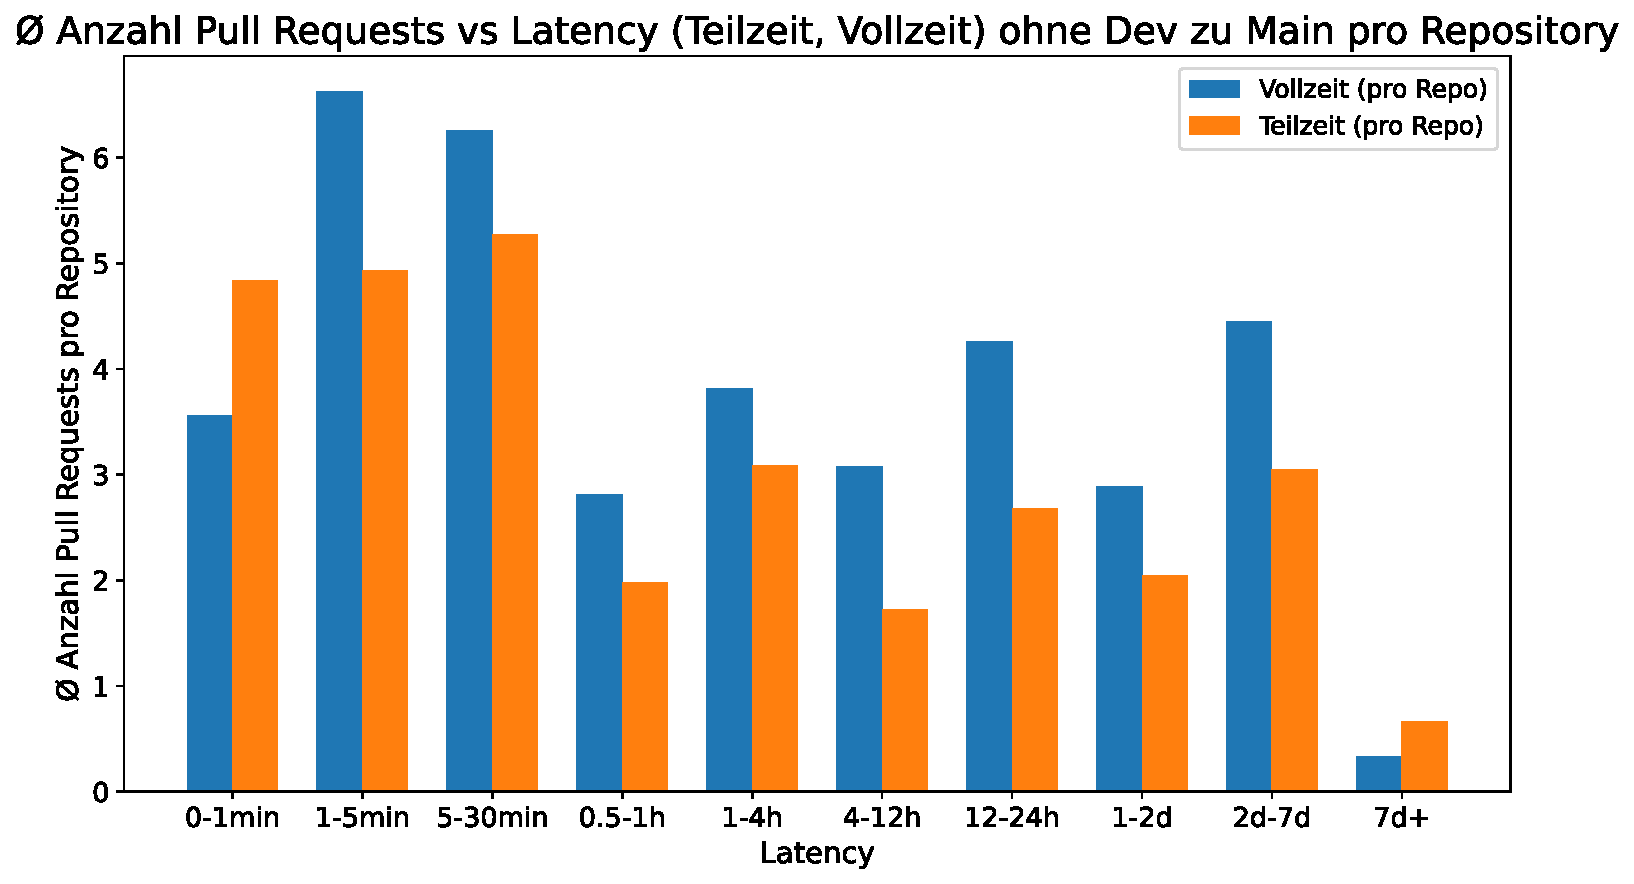
\includegraphics[width=\textwidth]{Figures/anz-avg-prs-vs-latency-tv-no-dev.pdf}
    \caption{Durchschnittliche Anzahl Pull-Requests vs. Latency (Teilzeit, Vollzeit) ohne Dev zu Main}
    \label{fig:anz-avg-prs-vs-latency-tv-no-dev}
\end{figure}


Ebenfalls bleibt das Bild, nach der Entfernung der Pull-Requests von Dev-Branches, in Bezug auf die Churn-Grössen weitgehend unverändert.

Die \autoref{fig:anz-prs-vs-churn-size-tz-vz-ohne-dev} zeigt die durchschnittliche Anzahl von Pull-Requests pro Repository gruppiert nach ihrer Churn-Grösse, ohne Dev-Branch-Merges. Es ist ersichtlich, dass die Vollzeitklassen in allen Churn-Kategorien tendenziell mehr Pull-Requests pro Repository erstellen als die Teilzeitklassen. Besonders in den Kategorien M (50–199 Änderungen) und L (200–999 Änderungen) ist der Unterschied deutlich ausgeprägt. In den Kategorien XS (0–9 Änderungen) und S (10–49 Änderungen) ist der Abstand zwischen Teilzeit- und Vollzeitklassen zwar etwas geringer, aber immer noch zugunsten der Vollzeitklassen.

\begin{figure}[htbp]
    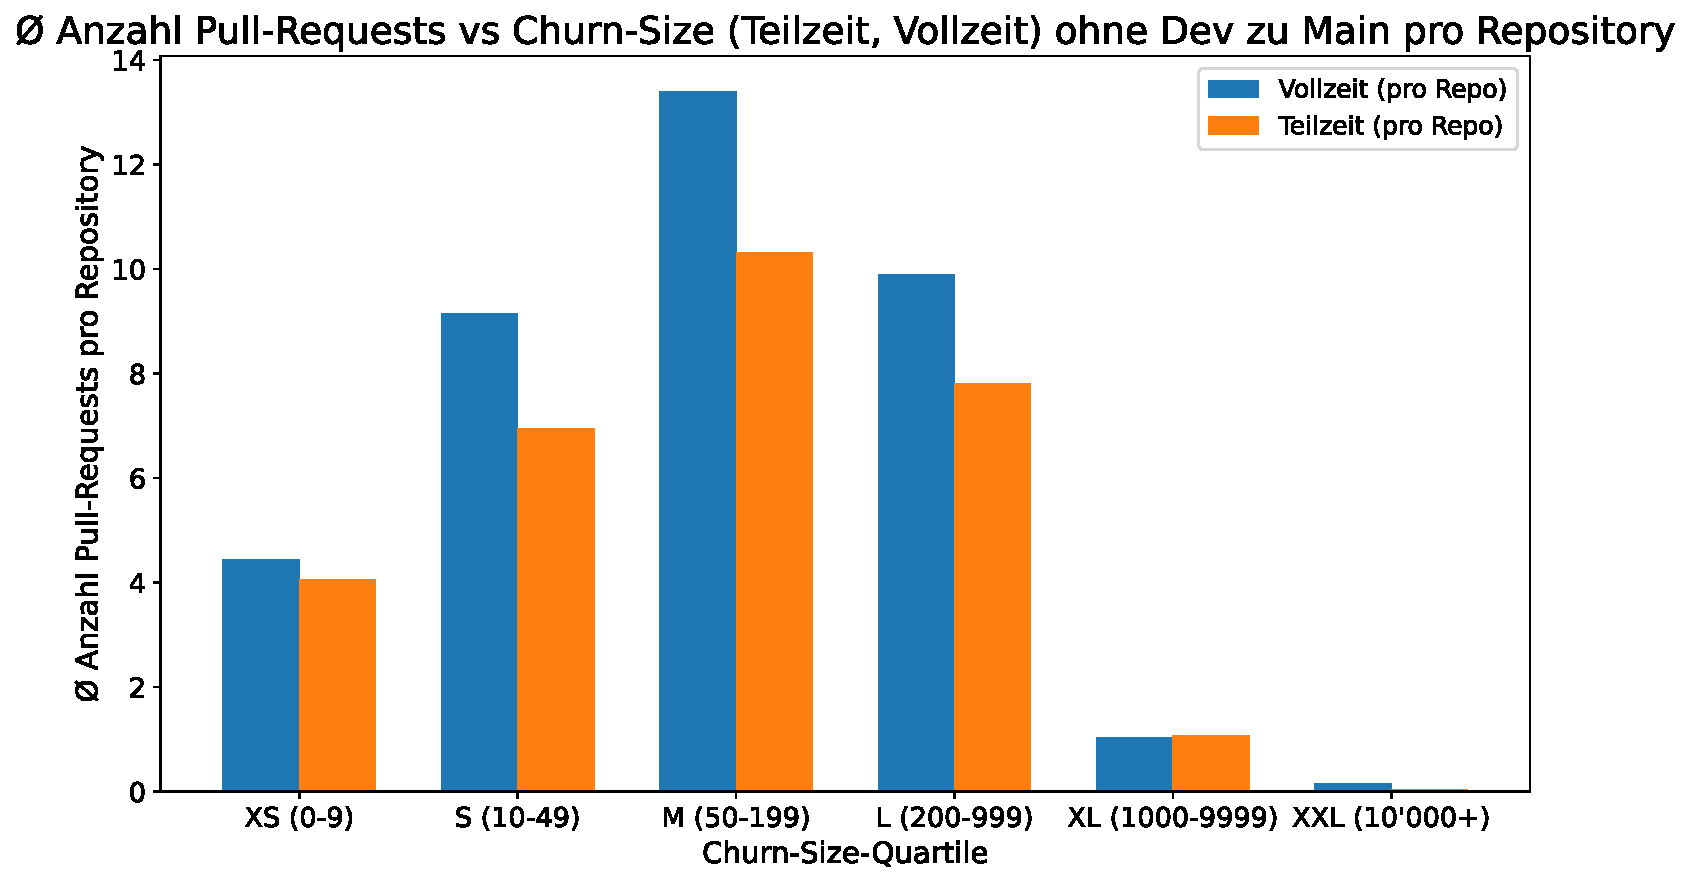
\includegraphics[width=\textwidth]{Figures/avg-anz-prs-vs-churn-size-tz-vz-pro-repo-ohne-dev.pdf}
    \caption{Durchschnittliche Anzahl Pull-Requests vs. Churn-Grösse (Teilzeit, Vollzeit) ohne Dev zu Main pro Repository}
    \label{fig:anz-prs-vs-churn-size-tz-vz-ohne-dev}
\end{figure}


Zum Vergleich zeigt die \autoref{fig:anz-prs-vs-churn-size-tz-vz-nur-dev} nur die PRs, die von Dev-Branches auf Main-Branches gemerged wurden. Hier zeigt sich, dass diese Pull-Requests insbesondere in den grösseren Churn-Kategorien (L bis XXL) auftreten. Auffällig ist zudem, dass in dieser Betrachtung die Vollzeitstudierenden mehr grosse Dev-Branch Pull-Requests erzeugen als die Teilzeitstudierenden.

\begin{figure}[htbp]
    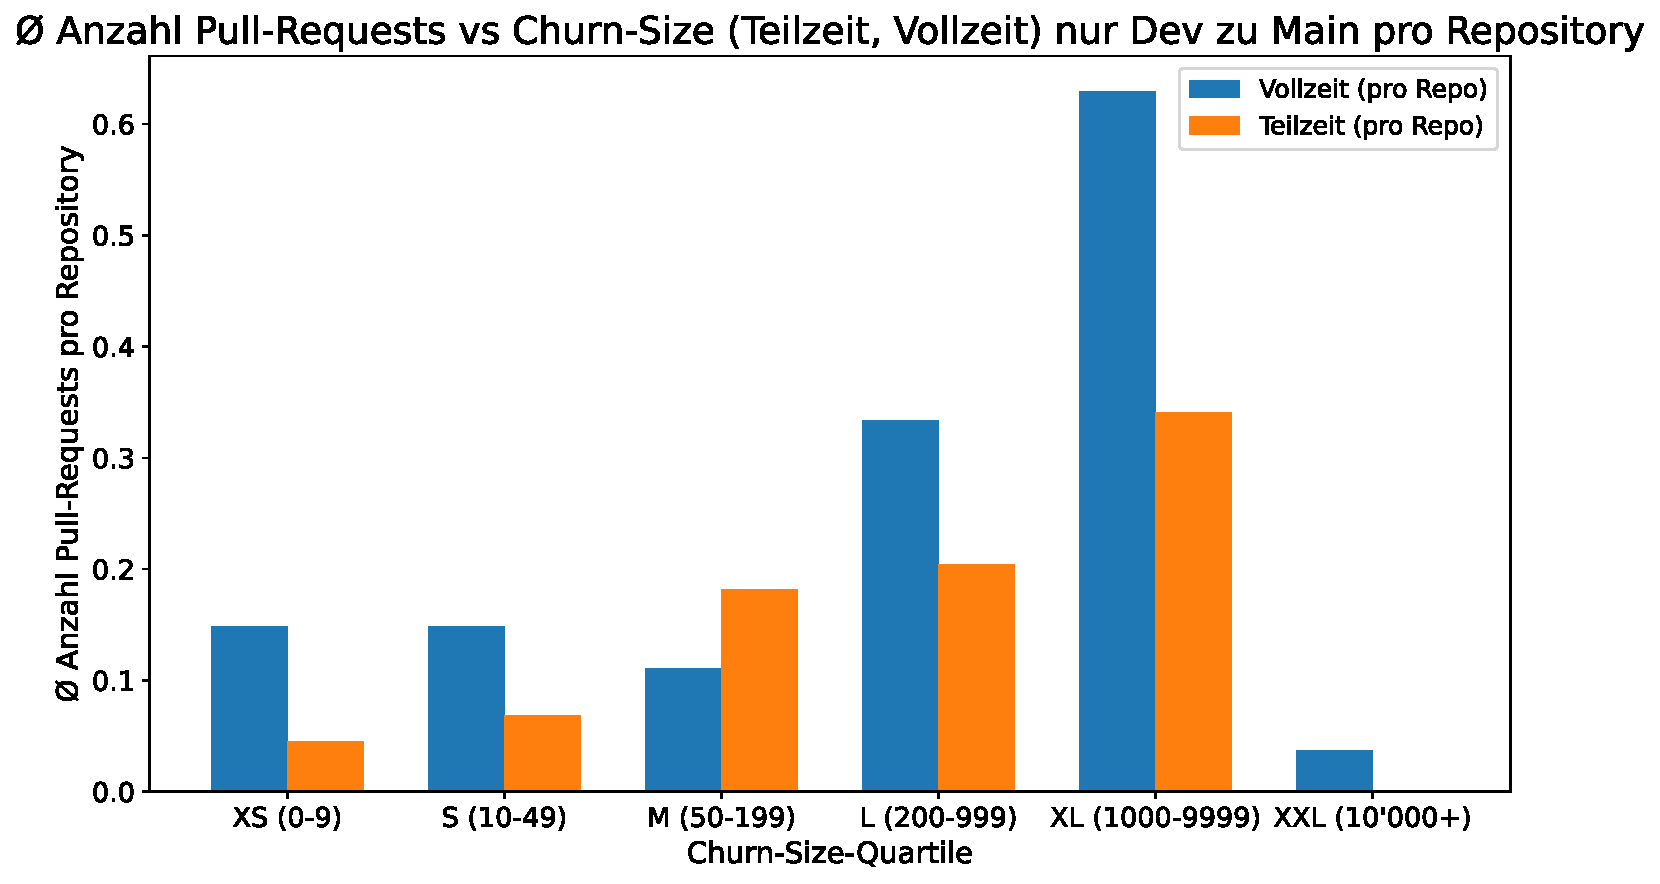
\includegraphics[width=\textwidth]{Figures/avg-anz-prs-vs-churn-size-tz-vz-pro-repo-nur-dev.pdf}
    \caption{Durchschnittliche Anzahl Pull-Requests vs. Churn-Grösse (Teilzeit, Vollzeit) nur Dev zu Main pro Repository}
    \label{fig:anz-prs-vs-churn-size-tz-vz-nur-dev}
\end{figure}

\subsection{Zusammenfassung}

Die Analyse zeigt Unterschiede zwischen Teilzeit- und Vollzeitstudierenden in der Pull-Request-Nutzung. Vollzeitstudierende erstellen im Durchschnitt mehr Pull-Requests, haben umfangreichere Änderungen und eine konsistentere Bearbeitungszeit. Teilzeitstudierende hingegen weisen stärkere Schwankungen bezüglich der Latencies auf. Auffällig häufig kommen dabei sehr kurze sowie sehr lange Bearbeitungszeiten vor. Vollzeitstudierende dominieren insbesondere bei grösseren Pull-Requests, während Teilzeitstudierende kleinere Änderungen häufiger schnell bearbeiten. Der Einfluss der Dev-Branch-Merges auf die Latency sowie die Churn-Verteilung ist dabei nur gering. 
%----------------------------------------------------------------------------------------
% SECTION 6
%----------------------------------------------------------------------------------------

\section{Korrelationsanalyse verschiedener Metriken}
\label{sec:Korrelationsanalyse}
In diesem Kapitel wird die \fref{forschungsfrage6} "\textit{Welche Unterschiede zeigen sich in den Repository-Metriken
zwischen den Studentenprojekten und professionellen GitHub-Organisationen?}" untersucht. Dazu werden zunächst die Metriken der Racetrack-Projekte analysiert und eine Korrelationsmatrix erstellt und anschliessend mit den Open-Source-Projekten der GitHub-Organisationen Ubique Innovation AG, Schweizerische Bundesbahnen (SBB) und Zalando SE verglichen.
\subsection{Korrelationsanalyse der Racetrack-Repositories}
Die Korrelationsmatrix der Racetrack-Projekte ist in \autoref{fig:korrelationsmatrix-racetrack} dargestellt. Auffällig ist die starke positive Korrelation, welche zwischen Churn und Commits (0.62) sowie zwischen Churn und Changed Files Count (0.70) besteht. 

\begin{figure}[htbp]
    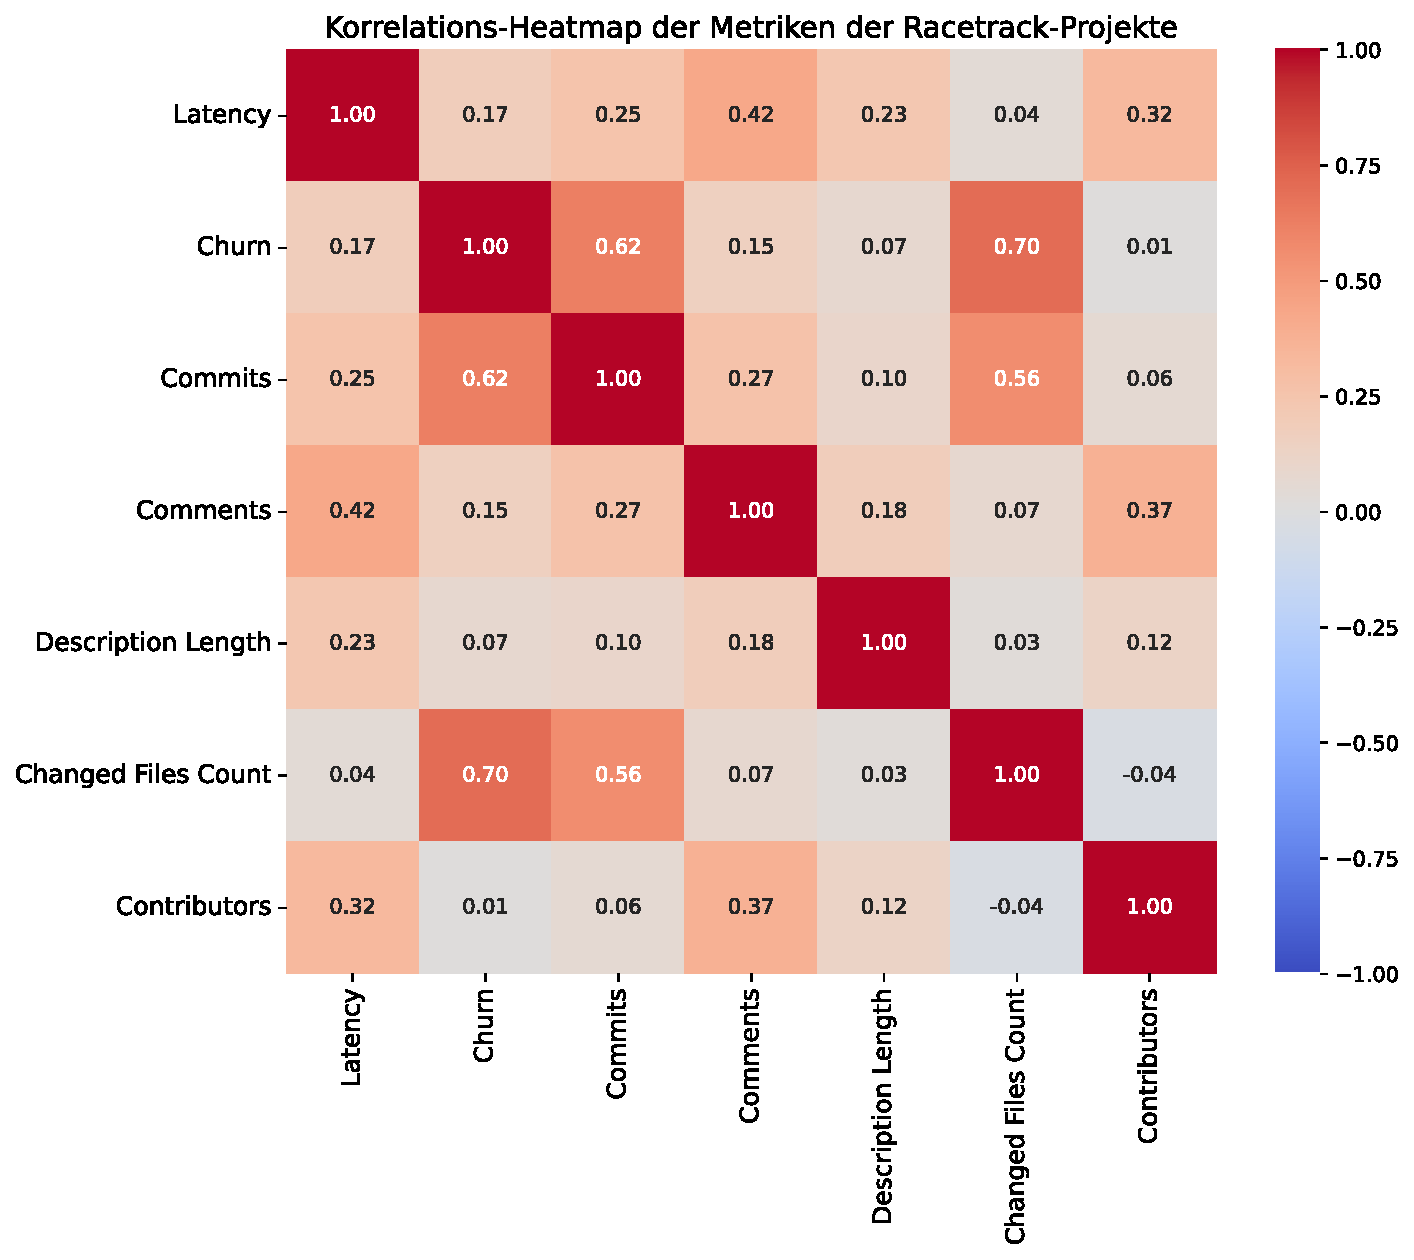
\includegraphics[width=\textwidth]{Figures/racetrack-korrelationsmatrix.pdf}
    \caption{Korrelations-Heatmap der Metriken der Racetrack-Repositories}
    \label{fig:korrelationsmatrix-racetrack}
\end{figure}


\subsection{Vergleich mit professionellen GitHub-Organisationen}
Zur besseren Einordnung der Ergebnisse der Racetrack-Projekte erfolgt nun ein Vergleich mit drei professionellen GitHub-Organisationen unterschiedlicher Grössenordnung. Die Auswahl der drei GitHub-Organisationen Ubique Innovation AG, Schweizerische Bundesbahnen (SBB) und Zalando wird in \autoref{sec:VorstellungGithubOrgs} erläutert. 


\subsubsection{Ubique Innovation AG}
Die Korrelationsmatrix von Ubique (siehe 
\autoref{fig:korrelationsmatrix-ubique}) zeigt ebenfalls starke positive Zusammenhänge zwischen Churn, Commits (0.64) und Changed Files Count (0.70). Jedoch zeigt sich bei Ubique eine positive Korrelation zwischen Latency und Comments (0.28), was auf umfangreichere Reviews bei längeren Bearbeitungszeiten hindeutet.

\begin{figure}[htbp]
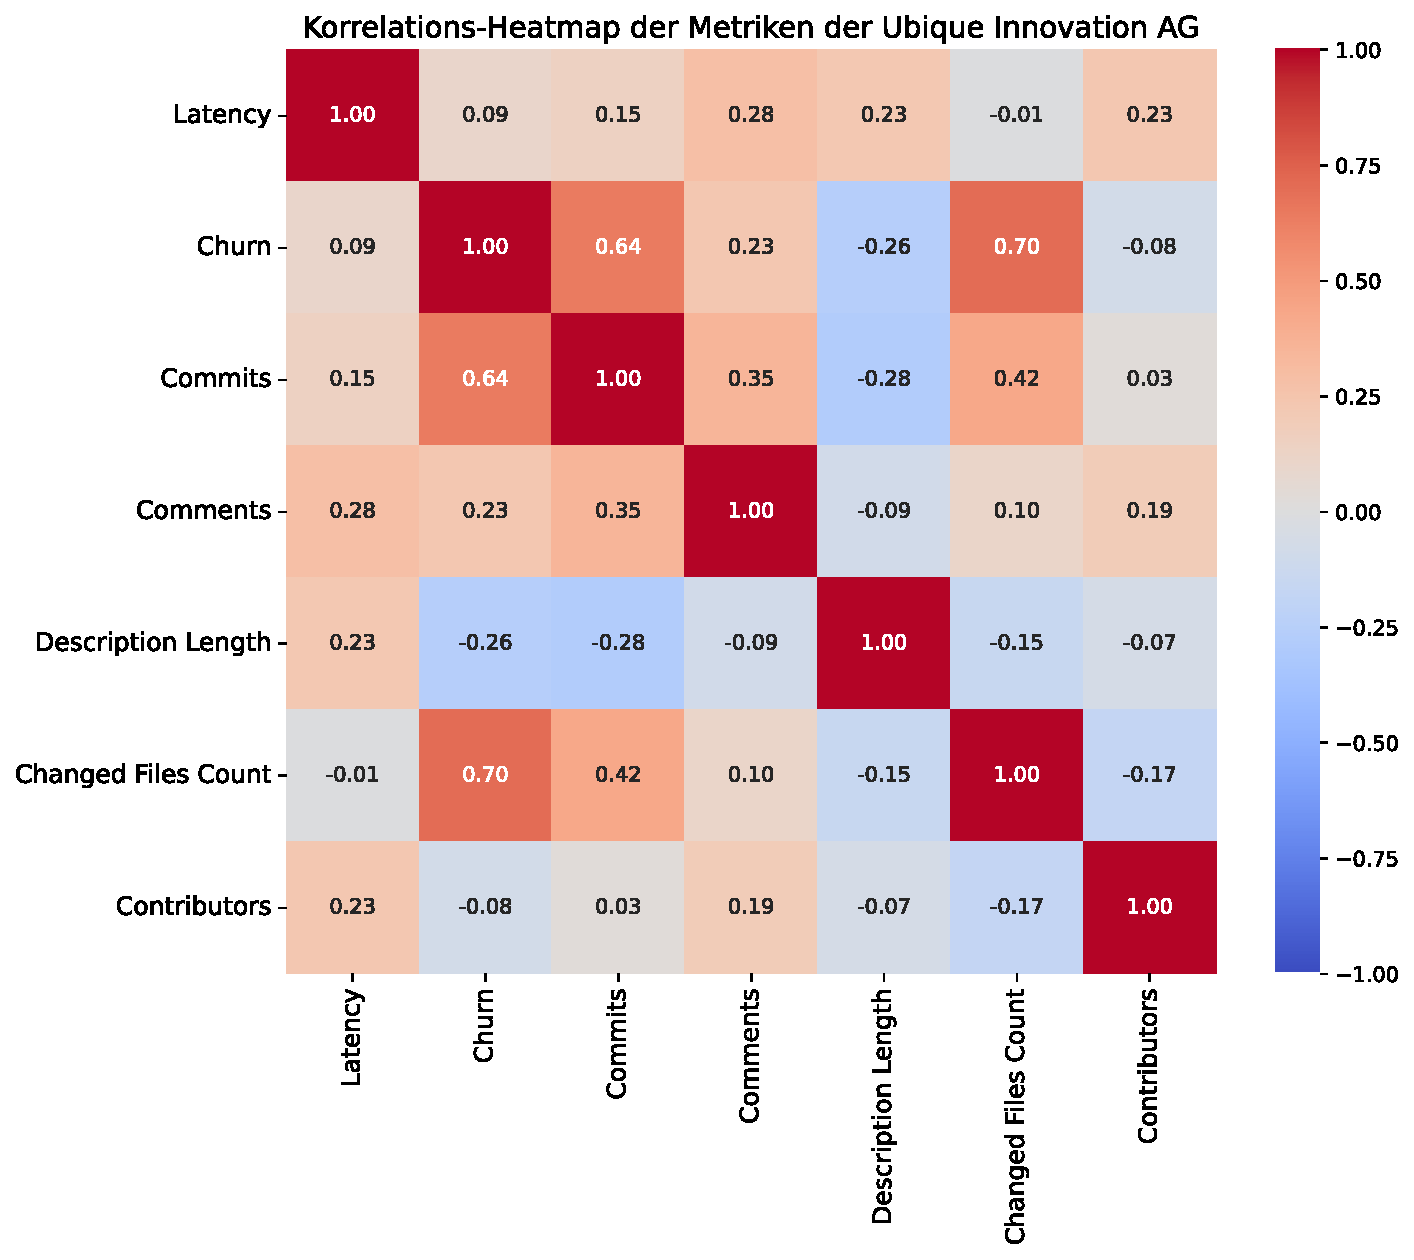
\includegraphics[width=\textwidth]{Figures/ubique-korrelationsmatrix.pdf}
\caption{Korrelations-Heatmap der Metriken von Ubique Innovation AG}
\label{fig:korrelationsmatrix-ubique}
\end{figure}


Um die Unterschiede zwischen den Racetrack-Repositories und den untersuchten OSS-Repositories besser zu erkennen, wurde eine Differenzanalyse durchgeführt. Hierbei wurden die Differenzen der einzelnen Korrelationen berechnet und in einer Heatmap dargestellt. Die Differenzanalyse zwischen Racetrack und Ubique (siehe \autoref{fig:diff-korrelationsmatrix-racetrack-ubique}) zeigt, dass die Racetrack-Projekte stärkere positive Korrelationen zwischen Description Length und Commits (0.38) sowie Description Length und Churn (0.34) aufweisen.

\begin{figure}[htbp]
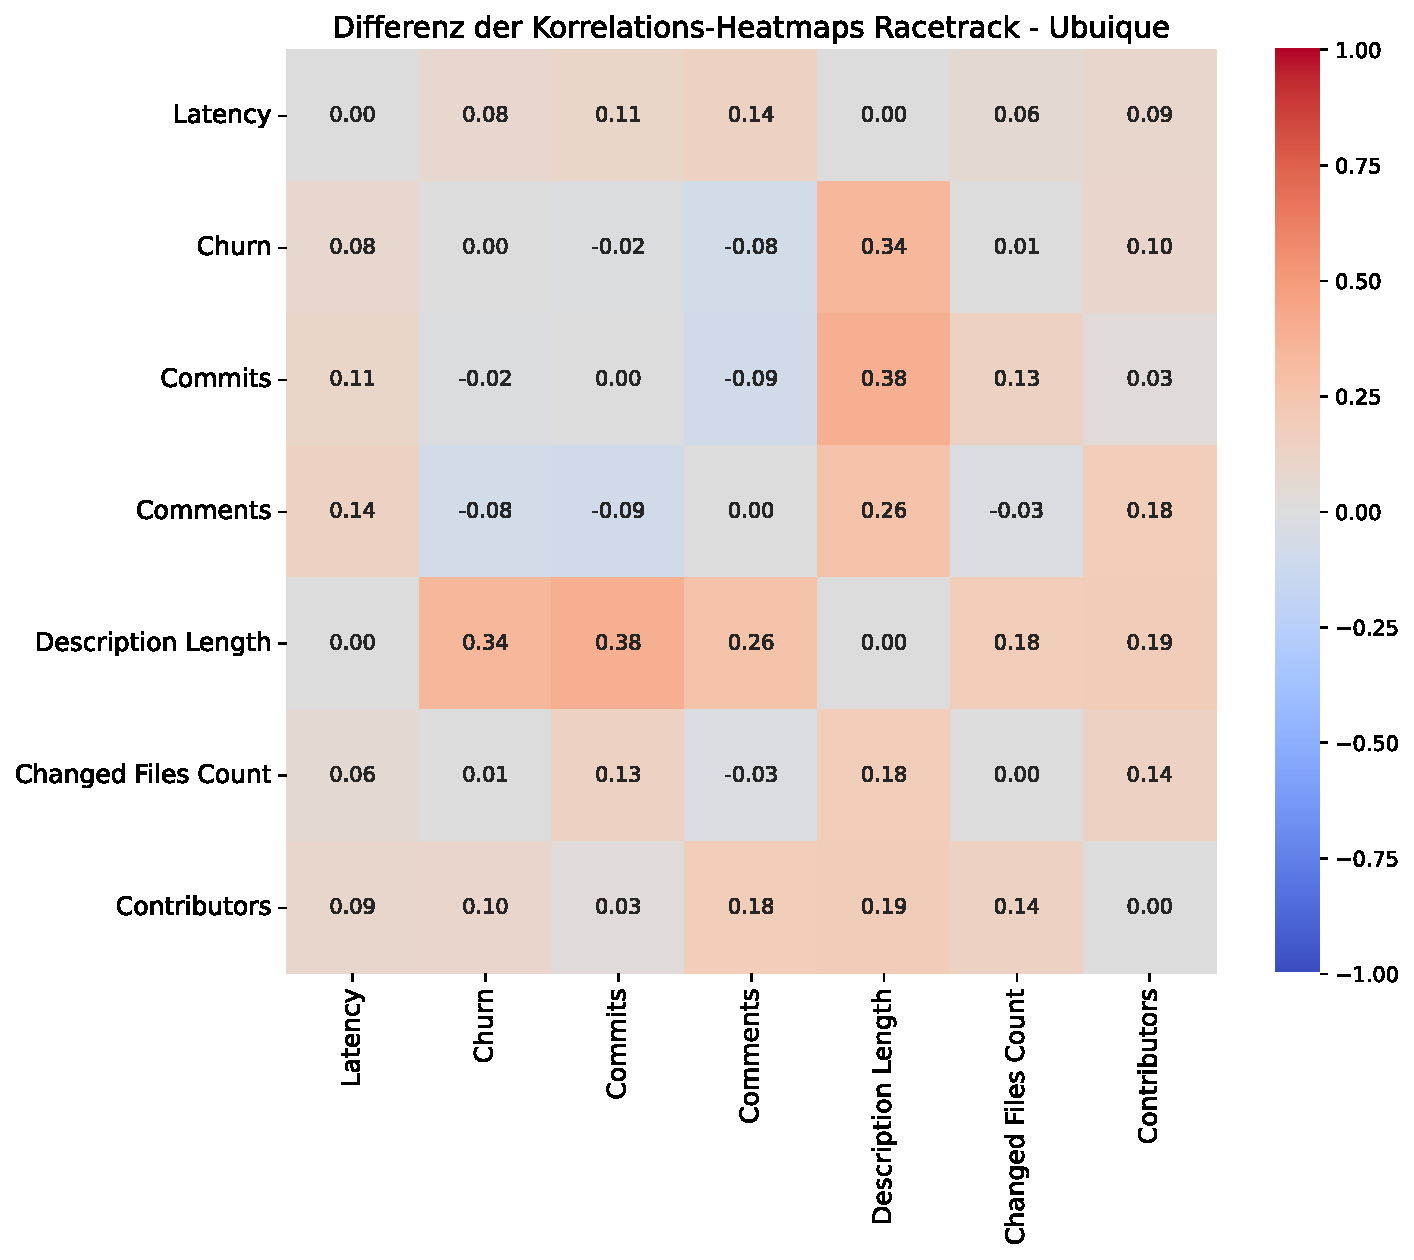
\includegraphics[width=\textwidth]{Figures/diff-korrelationsmatrix-racetrack-ubique.pdf}
\caption{Differenz der Korrelations-Heatmaps der Racetrack Repositories und der Ubique Innovation GitHub Organisation}
\label{fig:diff-korrelationsmatrix-racetrack-ubique}
\end{figure}


\subsubsection{Schweizerische Bundesbahnen (SBB)}
Die Korrelationsmatrix der SBB (\autoref{fig:korrelationsmatrix-sbb}) weist ebenfalls starke positive Korrelationen zwischen Churn und Commits (0.54) sowie Churn und Changed Files Count (0.81) auf. Auffällig bei der SBB ist die negative Korrelation zwischen Description Length und Commits (-0.33).

\begin{figure}[htbp]
    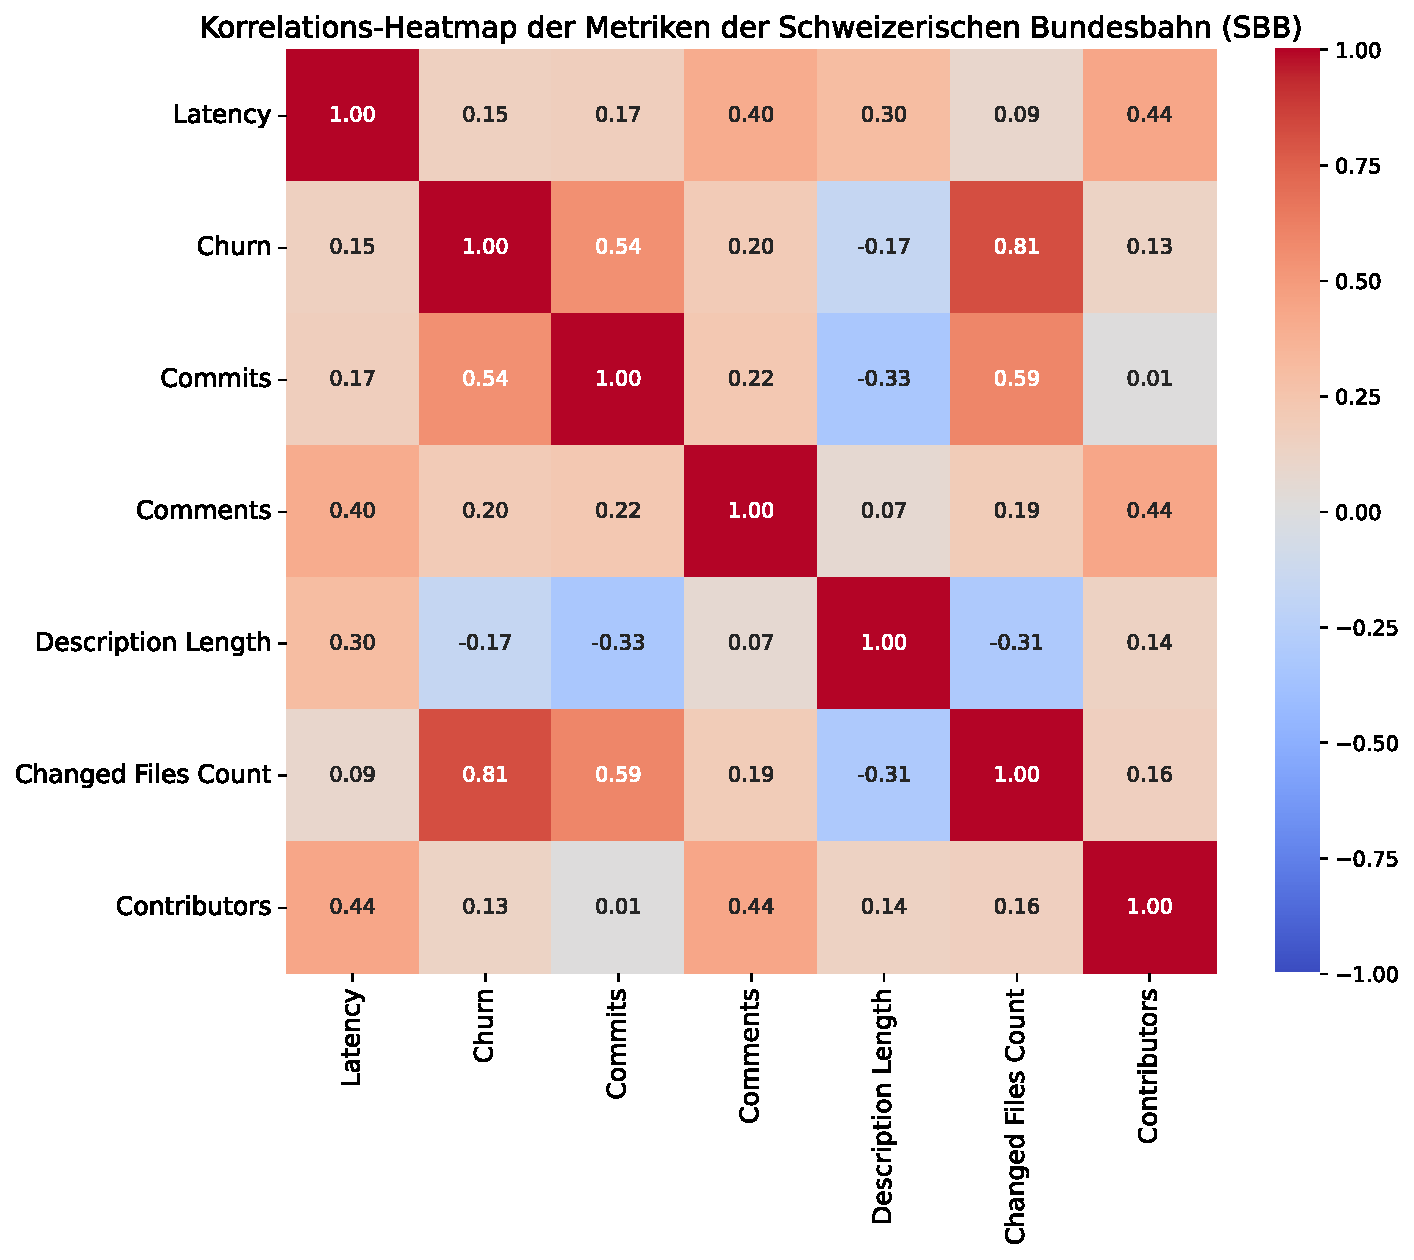
\includegraphics[width=\textwidth]{Figures/sbb-korrelationsmatrix.pdf}
    \caption{Korrelations-Heatmap der Metriken der Schweizerischen Bundesbahn (SBB)}
    \label{fig:korrelationsmatrix-sbb}
\end{figure}


Die Differenzanalyse zwischen Racetrack und SBB (\autoref{fig:diff-korrelationsmatrix-racetrack-sbb}) zeigt, dass Racetrack eine stärkere positive Korrelation zwischen Description Length und einigen Metriken wie Churn, Commits sowie eine schwächere Korrelation mit der Anzahl Comments aufweist.

\begin{figure}[htbp]
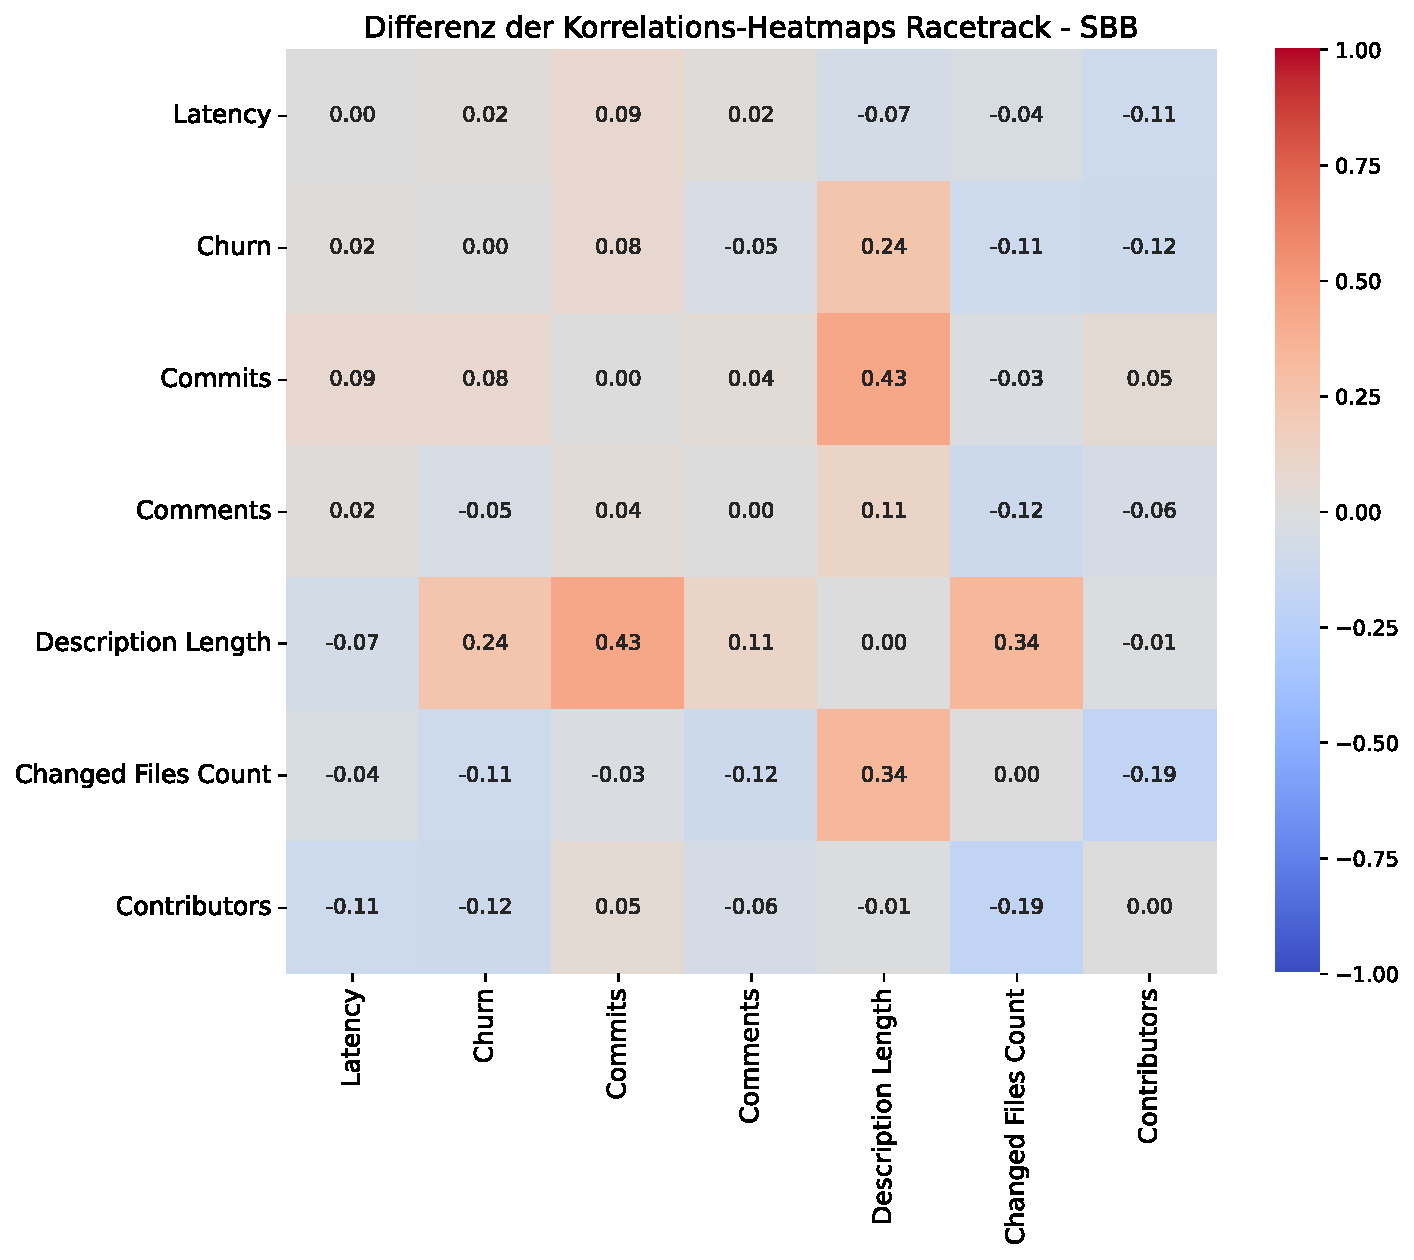
\includegraphics[width=\textwidth]{Figures/diff-korrelationsmatrix-racetrack-sbb.pdf}
\caption{Differenz der Korrelations-Heatmaps der Racetrack-Repositories und der SBB-GitHub-Organisation}
\label{fig:diff-korrelationsmatrix-racetrack-sbb}
\end{figure}



\subsubsection{Zalando SE}
Die Korrelationsmatrix von Zalando (\autoref{fig:korrelationsmatrix-zalando}) zeigt deutliche Unterschiede zu Racetrack, insbesondere eine starke negative Korrelation zwischen Churn und Description Length (-0.47), was darauf hindeutet, dass bei Zalando umfangreiche Änderungen oft weniger ausführlich beschrieben werden. Zudem zeigt sich eine positive Korrelation zwischen Churn und Changed Files Count (0.82), ähnlich wie bei den anderen Organisationen. Auch gibt es eine negative Korrelation zwischen Changed Files Count und Description Length (-0.41).

\begin{figure}[htbp]
    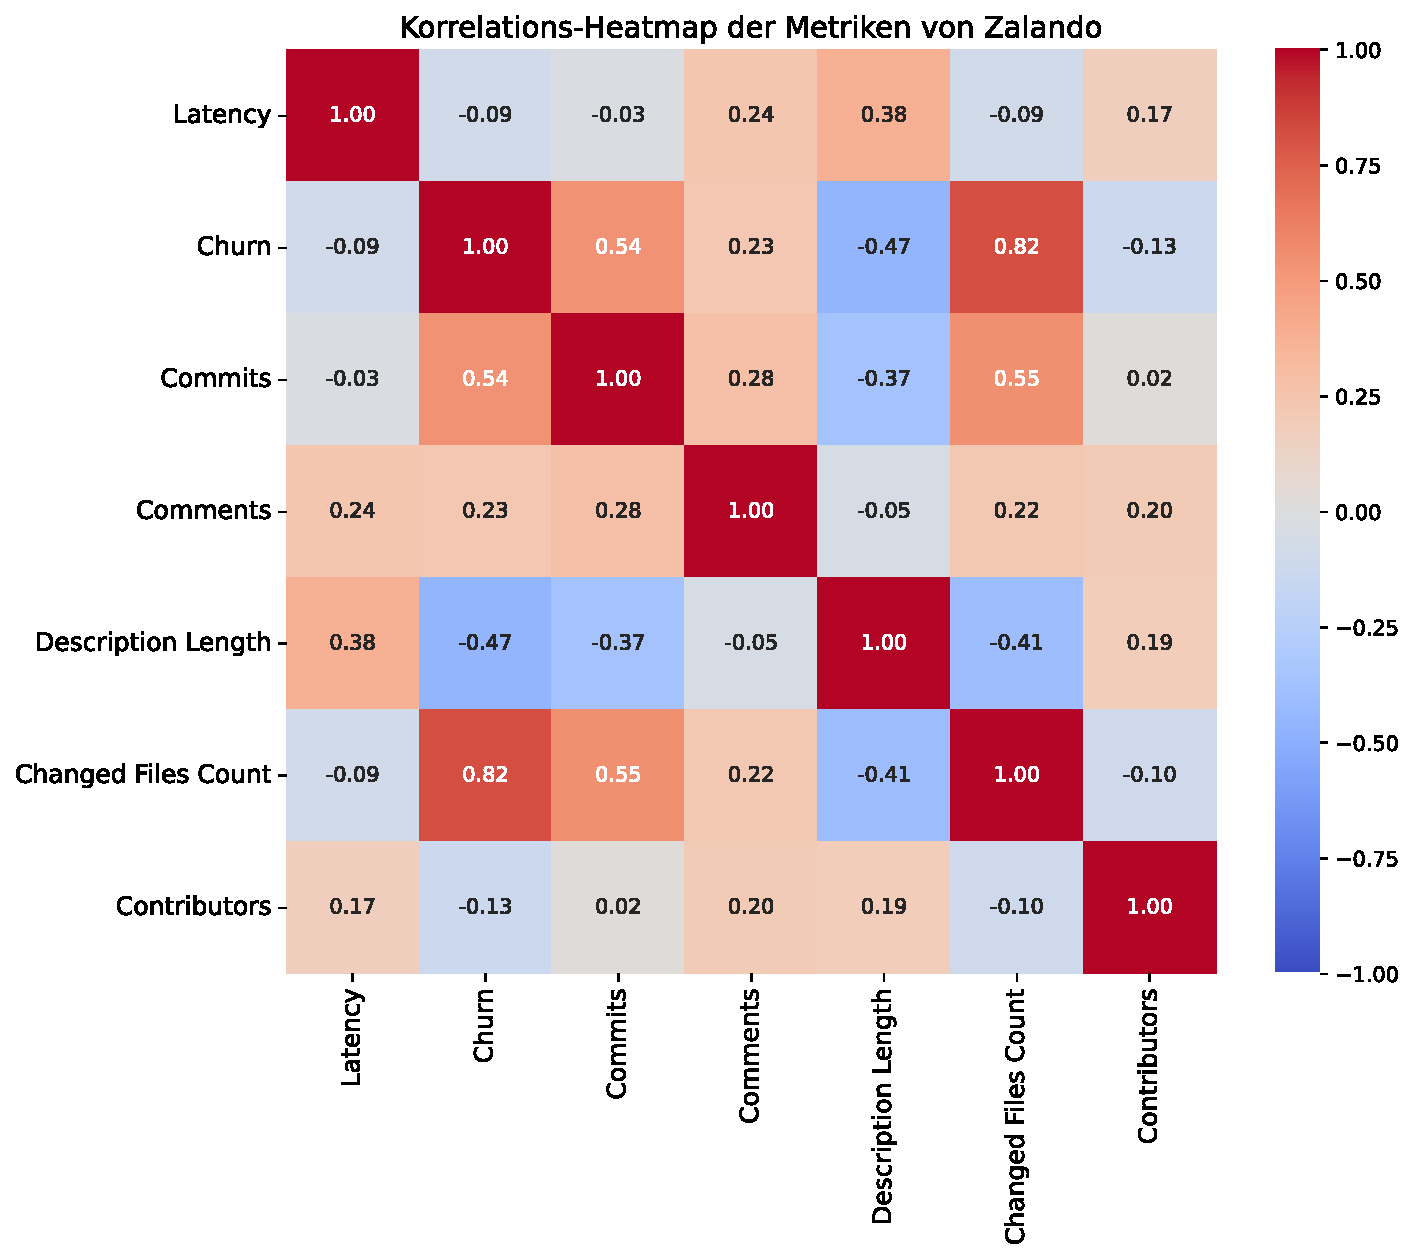
\includegraphics[width=\textwidth]{Figures/zalando-korrelationsmatrix.pdf}
    \caption{Korrelations-Heatmap der Metriken von Zalando}
    \label{fig:korrelationsmatrix-zalando}
\end{figure}

Die Differenzanalyse zwischen Racetrack und Zalando (\autoref{fig:diff-korrelationsmatrix-racetrack-zalando}) verdeutlicht, dass Racetrack im Gegensatz zu Zalando deutliche positive Korrelationen zwischen Description Length und sowohl Commits als auch Churn aufweist.

\begin{figure}[ht]
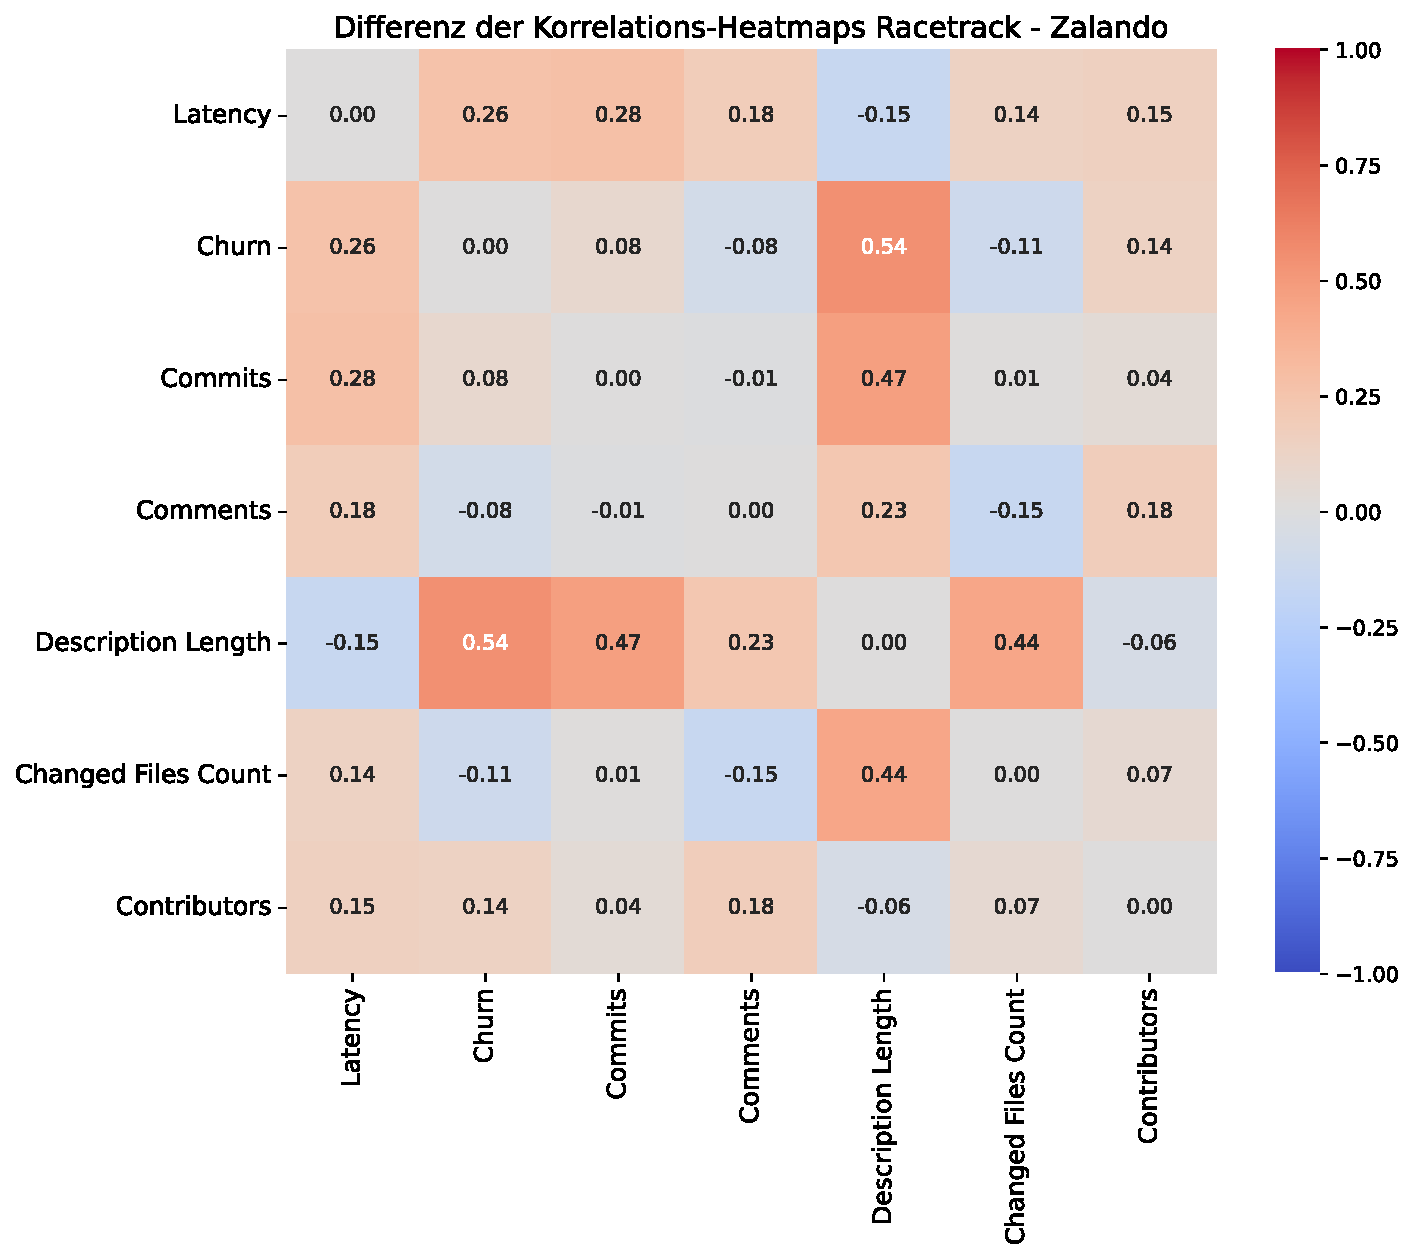
\includegraphics[width=\textwidth]{Figures/diff-korrelationsmatrix-racetrack-zalando.pdf}
\caption{Differenz der Korrelations-Heatmaps der Racetrack Repositories und der Zalando GitHub Organisation}
\label{fig:diff-korrelationsmatrix-racetrack-zalando}
\end{figure}



\subsection{Zusammenfassung}
Die Analyse zeigt, dass starke positive Korrelationen zwischen den Metriken Churn, Commits und Changed Files Count sowohl in den Racetrack-Projekten als auch in den professionellen GitHub-Organisationen vorhanden sind. Diese Korrelationen deuten darauf hin, dass umfangreiche Änderungen häufig mit vielen Commits und vielen veränderten Dateien einhergehen.

Unterschiede zeigen sich insbesondere bei der Korrelation mit der Metrik Description Length. In den Racetrack-Projekten stehen längere Pull-Request-Beschreibungen in positivem Zusammenhang mit umfangreicheren Änderungen und mehr Commits. 
In den professionellen Projekten hingegen, insbesondere bei Zalando, zeigt sich eine negative Korrelation zwischen Description Length und Churn. 

Zusammenfassend lässt sich zur \fref{forschungsfrage6} feststellen, dass zwar einige Metriken in den Racetrack und in professionellen Projekten ähnlich korrelieren, insbesondere im Bereich Churn, Commits und Changed Files Count, jedoch insbesondere die Beschreibungstexte der Pull-Requests unterschiedliche Zusammenhänge zu anderen Metriken aufweisen.





%----------------------------------------------------------------------------------------
% SECTION 7
%----------------------------------------------------------------------------------------

